%Pueden faltar
% Cambiar por travel por traversal.
% Actualizar imagenes
% Max array
% Mencionar que se usa comibining triangles

%%%%%%%%%%%%%%%%%%%%%%%%%%%%%%%%%%%%%%%%%%%%%%%%%%%%%%%%%%%%%%%%%%%%%
%%                                                                 %%
%% Please do not use \input{...} to include other tex files.       %%
%% Submit your LaTeX manuscript as one .tex document.              %%
%%                                                                 %%
%% All additional figures and files should be attached             %%
%% separately and not embedded in the \TeX\ document itself.       %%
%%                                                                 %%
%%%%%%%%%%%%%%%%%%%%%%%%%%%%%%%%%%%%%%%%%%%%%%%%%%%%%%%%%%%%%%%%%%%%%

%%\documentclass[referee,sn-basic]{sn-jnl}% referee option is meant for double line spacing

%%=======================================================%%
%% to print line numbers in the margin use lineno option %%
%%=======================================================%%

%%\documentclass[lineno,sn-basic]{sn-jnl}% Basic Springer Nature Reference Style/Chemistry Reference Style

%%======================================================%%
%% to compile with pdflatex/xelatex use pdflatex option %%
%%======================================================%%

%%\documentclass[pdflatex,sn-basic]{sn-jnl}% Basic Springer Nature Reference Style/Chemistry Reference Style

%%\documentclass[sn-basic]{sn-jnl}% Basic Springer Nature Reference Style/Chemistry Reference Style
\documentclass[lineno,pdflatex,sn-mathphys]{sn-jnl}% Math and Physical Sciences Reference Style
%%\documentclass[sn-aps]{sn-jnl}% American Physical Society (APS) Reference Style
%%\documentclass[sn-vancouver]{sn-jnl}% Vancouver Reference Style
%%\documentclass[sn-apa]{sn-jnl}% APA Reference Style
%%\documentclass[sn-chicago]{sn-jnl}% Chicago-based Humanities Reference Style
%%\documentclass[sn-standardnature]{sn-jnl}% Standard Nature Portfolio Reference Style
%%\documentclass[default]{sn-jnl}% Default
%%\documentclass[default,iicol]{sn-jnl}% Default with double column layout

%%%% Standard Packages
%%<additional latex packages if required can be included here>
%%%%
\usepackage{pdfpages}

\usepackage{subfigure} % subfiguras
%\usepackage{subcaption}
\usepackage{graphicx}
\usepackage{booktabs}


\usepackage[shortlabels]{enumitem} %cambiar


%%%%%=============================================================================%%%%
%%%%  Remarks: This template is provided to aid authors with the preparation
%%%%  of original research articles intended for submission to journals published 
%%%%  by Springer Nature. The guidance has been prepared in partnership with 
%%%%  production teams to conform to Springer Nature technical requirements. 
%%%%  Editorial and presentation requirements differ among journal portfolios and 
%%%%  research disciplines. You may find sections in this template are irrelevant 
%%%%  to your work and are empowered to omit any such section if allowed by the 
%%%%  journal you intend to submit to. The submission guidelines and policies 
%%%%  of the journal take precedence. A detailed User Manual is available in the 
%%%%  template package for technical guidance.
%%%%%=============================================================================%%%%

\jyear{2021}%

%% as per the requirement new theorem styles can be included as shown below
\theoremstyle{thmstyleone}%
\newtheorem{theorem}{Theorem}%  meant for continuous numbers
\newtheorem{lemma}{Lemma}%  meant for continuous numbers
%%\newtheorem{theorem}{Theorem}[section]% meant for sectionwise numbers
%% optional argument [theorem] produces theorem numbering sequence instead of independent numbers for Proposition
\newtheorem{proposition}[theorem]{Proposition}% 
%%\newtheorem{proposition}{Proposition}% to get separate numbers for theorem and proposition etc.

\theoremstyle{thmstyletwo}%
\newtheorem{example}{Example}%
\newtheorem{remark}{Remark}%

\theoremstyle{thmstylethree}%
\newtheorem{definition}{Definition}%

\raggedbottom
%%\unnumbered% uncomment this for unnumbered level heads
%\usepackage{setspace}   %Allows double spacing with the \doublespacing command
%\doublespacing 
\begin{document}

\title[POLYLLA: Polygonal meshing algorithm based on terminal-edge regions]{POLYLLA: Polygonal meshing algorithm based on terminal-edge regions}

%%=============================================================%%
%% Prefix	-> \pfx{Dr}
%% GivenName	-> \fnm{Joergen W.}
%% Particle	-> \spfx{van der} -> surname prefix
%% FamilyName	-> \sur{Ploeg}
%% Suffix	-> \sfx{IV}
%% NatureName	-> \tanm{Poet Laureate} -> Title after name
%% Degrees	-> \dgr{MSc, PhD}
%% \author*[1,2]{\pfx{Dr} \fnm{Joergen W.} \spfx{van der} \sur{Ploeg} \sfx{IV} \tanm{Poet Laureate} 
%%                 \dgr{MSc, PhD}}\email{iauthor@gmail.com}
%%=============================================================%%

\author*[1]{\fnm{Sergio} \sur{Salinas}}\email{ssalinas@dcc.uchile.cl}
\equalcont{These authors contributed equally to this work.} 
\author*[1]{\fnm{Nancy} \sur{Hitschfeld-Kahler} \dgr{} }\email{nancy@dcc.uchile.cl}
\equalcont{These authors contributed equally to this work.}
\author[2]{\fnm{Alejandro} \sur{Ortiz-Bernardin} \dgr{}}\email{aortizb@uchile.cl}
\author[3]{\fnm{Hang} \sur{Si} \dgr{}}\email{si@wias-berlin.de}


\affil*[1]{\orgdiv{Department of Computer Sciences}, \orgname{Universidad de Chile}, \orgaddress{\\\street{Av. Beauchef 851}, \city{Santiago}, \postcode{8370456}, \state{RM}, \country{Chile}}}

\affil[2]{\orgdiv{Computational and Applied Mechanics Laboratory, Department of Mechanical Engineering}, \orgname{Universidad de Chile}, \orgaddress{\street{Av. Beauchef 851}, \city{Santiago}, \postcode{8370456}, \state{RM}, \country{Chile}}}

\affil[3]{\orgdiv{Numerical Mathematics and Scientific Computing}, \orgname{Weierstrass Institute for Applied Analysis and Stochastics}, \orgaddress{\street{Mohrenstr. 39}, \city{Berlin}, \postcode{10117}, \state{Berlin}, \country{Germany}}}



%%==================================%%
%% sample for unstructured abstract %%
%%==================================%%

\abstract{This paper presents an algorithm to generate a new kind of polygonal mesh obtained  from triangulations. Each polygon is built from a terminal-edge region surrounded by edges that are not the longest-edge of any of the two triangles that share them. The algorithm is termed Polylla and is divided into three phases.  The first phase consists of labeling each edge of the input triangulation according to its size; the second phase builds polygons (simple or not) from terminal-edges regions using the label system; and the third phase transforms each non simple polygon into simple ones. The final mesh contains polygons with convex and non convex shape. Since Voronoi based meshes are currently the most used polygonal meshes, we compare some geometric properties of our meshes against constrained Voronoi meshes. Several experiments were run to compare the shape and size of polygons, the number of final mesh points and polygons. For the same input, Polylla meshes contain less polygons than Voronoi meshes and the algorithm is simpler and faster than the algorithm to generate constrained Voronoi meshes. Finally, we have validated  Polylla meshes by solving the Laplace equation on an L-shaped domain using the Virtual Element Method (VEM). We show that the numerical performance of the VEM using  Polylla meshes and Voronoi meshes is similar.}

%%================================%%
%% Sample for structured abstract %%
%%================================%%

% \abstract{\textbf{Purpose:} The abstract serves both as a general introduction to the topic and as a brief, non-technical summary of the main results and their implications. The abstract must not include subheadings (unless expressly permitted in the journal's Instructions to Authors), equations or citations. As a guide the abstract should not exceed 200 words. Most journals do not set a hard limit however authors are advised to check the author instructions for the journal they are submitting to.
% 
% \textbf{Methods:} The abstract serves both as a general introduction to the topic and as a brief, non-technical summary of the main results and their implications. The abstract must not include subheadings (unless expressly permitted in the journal's Instructions to Authors), equations or citations. As a guide the abstract should not exceed 200 words. Most journals do not set a hard limit however authors are advised to check the author instructions for the journal they are submitting to.
% 
% \textbf{Results:} The abstract serves both as a general introduction to the topic and as a brief, non-technical summary of the main results and their implications. The abstract must not include subheadings (unless expressly permitted in the journal's Instructions to Authors), equations or citations. As a guide the abstract should not exceed 200 words. Most journals do not set a hard limit however authors are advised to check the author instructions for the journal they are submitting to.
% 
% \textbf{Conclusion:} The abstract serves both as a general introduction to the topic and as a brief, non-technical summary of the main results and their implications. The abstract must not include subheadings (unless expressly permitted in the journal's Instructions to Authors), equations or citations. As a guide the abstract should not exceed 200 words. Most journals do not set a hard limit however authors are advised to check the author instructions for the journal they are submitting to.}

\keywords{Polygonal mesh,Terminal-edge region, Virtual element method, Delaunay triangulations}

%%\pacs[JEL Classification]{D8, H51}

%%\pacs[MSC Classification]{35A01, 65L10, 65L12, 65L20, 65L70}

\maketitle

\section*{Article Highlights}

\begin{itemize}
%    \item Please provide three short bullet points (maximum of 120 characters each) summarizing the key findings and implications of the paper. These should be presented in non-technical language and not repeat verbatim text found in the abstract. They should be placed beneath the abstract under the heading of ‘Article Highlights’.
\item A simple and automatic tool to generate polygonal meshes 
composed of convex or/and non-convex polygons. %, fitting exactly the input domain and respecting the initial point distribution 
\item The polygonal meshes are composed of less polygons and points than constrained Voronoi meshes for the same input 
\item A new kind of polygonal meshes  for the virtual element method. %Currently, constrained Voronoi meshes are used.


%    \item \textcolor{blue}{New algorithm to generate polygonal meshes of arbitrary shape, using any kind of triangulation as input, adaptable to any kind of geometry, no addition of extra points and with a data structure to an easy implementation to all language programmings.}
%    \item \textcolor{blue}{Geometric analysis and comparison with Voronoi diagram based meshes, in order to show Polylla meshes as an better alternative to Voronoi diagram in case of need arbitrary shape polygonal meshes.}
 %   \item \textcolor{blue}{Validation of Polylla mesh in L-shape domain using the Virtual Element Method with semiuniform and ramdon position set of vertices. }
\end{itemize}

\section{Introduction}\label{sec1}

Meshes composed of  triangles and quadrilaterals are common in simulations using the Finite Element Method (FEM). One of the main requirements is that polygons (elements)  need to obey specific quality criteria such as  angles not too large or small, or reasonable aspect ratio and  area,  among others. To fulfill these criteria, sometimes the insertion of a large number of points and elements is required in order to properly model a domain, increasing the time needed to make a simulation. New methods such as the Virtual Element Method (VEM)~\cite{Basisprinciples,Brezzi2015} can use any polygon as basic cell. Our main research interest is to explore how far the VEM can handle non-convex and convex polygons and still be able to compute accurate simulation results. Our goal is to build a new tool that allows the VEM community~\cite{Wriggers2019} to model and simulate more complex problems than before, both in 2D and 3D.


In this context, the VEM presents an opportunity to explore new kind of polygonal meshes and new algorithms to generate them. 
Our main research questions are: Can terminal-edge regions~\footnote{A terminal-edge region is formed by all triangles whose Longest-Edge Propagation Path (Lepp)~\cite{Rivara97} share the same terminal-edge.} be adapted to be used as good basic cells for polygonal numerical methods such as the VEM? Do this kind of meshes require less polygons to model the same problem than polygonal meshes based on the Voronoi diagram? Our hypotheses are: (i) Terminal-edge regions can be transformed into simple polygons and used  as basic cells, (ii) the domain geometry can be fitted using less elements than constrained Voronoi meshes, (iii) this kind of polygonal meshes can be used with the VEM. 

In this paper, we propose an algorithm to generate meshes that adapt to a geometric domain specified through  Planar line straight graph (PLSG) using  polygons of any shape, and respecting the  point distribution given as input. The algorithm reads as input a triangulation and uses the concept of terminal-edge region as basis to build polygons. 
% Meshes based on triangles and quadrilaterals are common in simulations using the Finite Element Method (FEM). The problem is that polygons(elements) in FEM need to obey specific quality criteria, to avoid angles that are too large or small, or with sides of graded  length (aspect ratio criteria), etc. To fulfill these criteria, sometimes the insertion of a large number of points and elements is required in order to properly model a domain, increasing the time needed to make the simulation. New methods as Virtual Element Method (VEM)~\cite{Basisprinciples,Brezzi2015} can use any polygon as basic cell. So, (i) the domain geometry can be fitted using  less elements than if only triangles and quadrilaterals are used, (ii) the required point density distribution is just that required by the simulation problem, and (iii) it should not be necessary to further improve the quality of the elements. We are currently researching how far the VEM can allow the simulation of more complex problems, in both 2D and 3D, in comparison to FEM~\cite{Wriggers2019}.
%---- Actualmente se usan las mallas basadas en el diagrama de voronoi, poligonos convexos. Se ha probado insertando poligonos aislados no convexos y evaluar si los resultados de la silumlacin son aun validos...Wriggers2017...
%---- las preguntas our research questions sn... podemos generar poligonos arbitrarios, automaticantes a partir de una geometria PSLG...y puntos interiores dados como input? .. ..
%In this paper we propose an algorithm to generate meshes with polygons of arbitrary shape (convex and non-convex,
Terminal-edge regions can generate non-simple polygons, so we also propose an algorithm to divide  them into simple ones. We  run several experiments to show  properties of these polygons and compare the generated meshes against constrained Voronoi meshes. Moreover, we  validate the polygonal meshes over a classical problem to show that these meshes can be used to solve problems with the VEM.   As an example, Fig. \ref{fig:logo} shows a polygonal mesh generated  with the algorithm proposed in this paper.

\begin{figure}
\centering
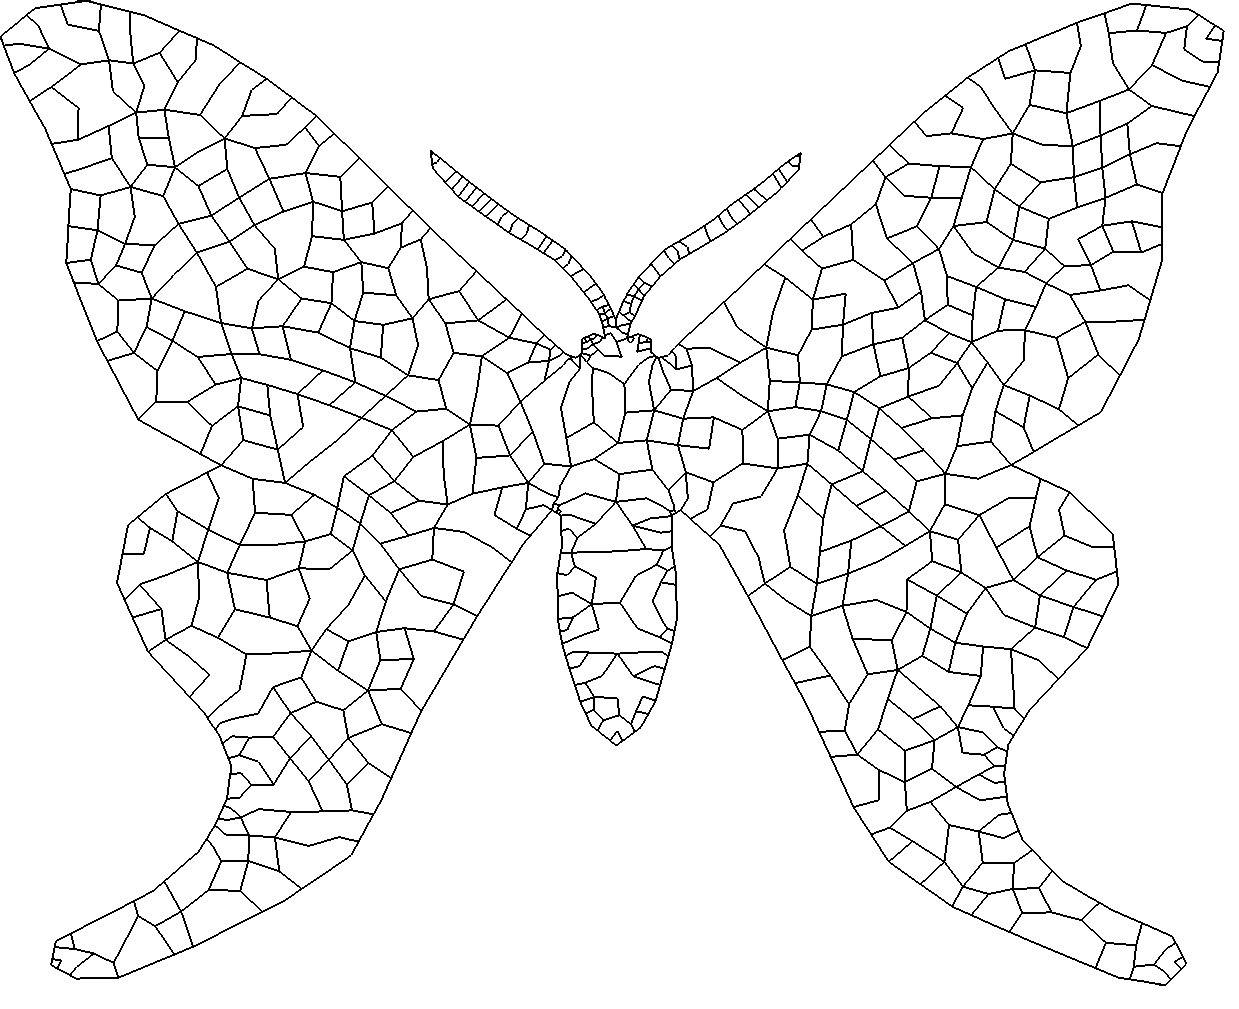
\includegraphics[width=0.8\linewidth]{polyllalogo2.png} 
%\includepdf[scale=0.75,angle=180]{pygal_nitauwu_135.svg}
\caption{Polygonal mesh of a Chilean moth (Polilla Venusta) composed of 513 polygons, 1351 vertices and 2455 edges. The original PLSG contains 616 points and segments. A conforming Delaunay triangulation with  maximum edge size of 160 was generated using Pygalmesh~\cite{Schlomer_pygalmesh_Python_interface}. The resulting triangulation contains 1351 vertices (the same of the output), 2083 triangles and 3432 edges.}
\label{fig:logo}    
\end{figure}

Any triangulation can be used as input but through this paper the polygonal meshes are generated from a Delaunay triangulation. It is known that  Delaunay triangulations are the ones that maximize the smallest angle among all the triangulations of a  point set. Since the proposed algorithm does not divide any input triangle, the smallest angle of the triangulation is a lower bound for the minimum interior angle of the polygonal mesh.


%
%\textcolor{blue}{Thus, the main contributions of this paper are: A simple and automatic way to generate polygonal meshes of arbitrary shape, without adding additional points to the initial input, and a evaluation of our meshes in tested simulations with the VEM.}

The main contributions of this paper are:
\begin{itemize}
    \item A simple and automatic tool to generate polygonal meshes composed of convex or/and non-convex polygons, fitting exactly the input domain and respecting the initial point distribution. 
    \item A new kind of polygonal meshes composed of less polygons and points than constrained Voronoi  meshes for the same input.
    \item The algorithm benefits from robust tools such as Detri2d or Triangle to generate the initial constrained Delaunay triangulation  in similar way some constrained Voronoi meshing algorithms do.  Voronoi meshing algorithms require to compute new points (Voronoi points),  cut non-bounded  Voronoi regions to fit the domain  and  insert new points at the domain boundary  to create the constrained Voronoi mesh. So the proposed algorithm is faster than the algorithm to generate constrained Voronoi meshes.
    
    %\item The algorithm benefits from robust tools such as Detri2d or Triangle to generate the input constrained Delaunay triangulation with the required mesh points in similar way  constrained Voronoi Diagram based meshes do. However Voronoi meshes require to cut not bounded Voronoi regions to fit the domain boundary and so, to insert new points.
\end{itemize}
\noindent
This paper is organized as follows: Section~\ref{sec:relatedwork} presents and discusses the-state-of-art;  Section~\ref{sec:basic} introduces the basic concepts  that explains the algorithm;  Section~\ref{sec:the_algorithm} describes the main steps of the proposed algorithm  and the used data structure; in Section~\ref{sec:experimental_evaluation} we analyse some geometric features of the generated meshes and gives a comparison against the constrained  Voronoi meshes; Section~\ref{sec:simulation_results} shows a preliminary assessment of the meshes in the Virtual Element Method (VEM) and Section~\ref{sec:conclusions} presents our  conclusions and ongoing work.

\section{Related work}
\label{sec:relatedwork}
%REVISAR Y DEJAR REFERENCIAS 2D

%\textcolor{blue}{To our knowledge, there are no algorithm to automatized the generation of 2D meshes with arbitrary shape for {\sc vem}}. 
%1. The literature review for mesh generation methods is rather sparse. I would have liked if the manuscript gave some historical context and mentioned some latest technologies on quad mesh generation, Voronoi-based mesh generation methods, and polygon mesh generation. 

% Important software actually used to generated polygonal meshes are Netgen~\cite{Schberl1997NETGENAA} and Triangle~\cite{triangle2d} for triangular Meshes, and Polymesher~\cite{PolyMesher2012} for Voronoi meshes among others meshers.}

Mesh generation refers to the methods used to discretize a geometric domain into smaller elements without overlap. Those methods has been widely studied due to their importance in science and engineering. Meshes are used in geographic information systems~\cite{PrinciplesGIS}, computer vision~\cite{JOHNSON1998261},  numerical methods~\cite{HOLE198827}, computer tomography~\cite{Zhang2007Automatic3M}, among other applications. Common methods used to generate unstructured polygon meshes are the Delaunay methods \cite{cheng2013delaunay}, Voronoi diagram methods \cite{yan:hal-00647979, 2dcentroidalvoro, PolyMesher2012}, advancing front method \cite{lohner1996progress, Schberl1997NETGENAA}, quadtree based methods \cite{BERN1994384, bommes2013quad, Liang2013AnOD} and hybrids methods \cite{owen1999q, ito2002unstructured}, among others. In general, meshing algorithms can be classified into two groups \cite{owen1998survey, johnen2016indirect}: (i) direct algorithms:  meshes are generated from the input geometry, and (ii) indirect algorithms: meshes are generated starting from an input mesh, typically an initial triangle mesh. Indirect methods is a common approach to generate quadrilateral meshes by mixing triangles of an initial triangulation ~\cite{LeetreetoQuad, BlossonQuad, Merhof2007Aniso-5662}. The advantage of using indirect methods is that currently triangular meshes are easy to generate because several robust open source and free tools~\cite{triangle2d, Detri2, qhull,  cgal:y-t2-21b} are available. Polylla mesh generation is an indirect method as it is based  on mixing triangles from an initial triangulation. 

In standard FEM, the most used 2D meshes are triangulations~\cite{triangle2d,Detri2, chew1} and quadrilateral meshes~\cite{Canann98, Lee20031055, Owen98advancingfront}. 2D Mixed meshes composed of triangles and quadrilaterals have also been used, but are not so common as the previous ones~\cite{jaillet2021}. Other numerical methods such as  the Voronoi Cell Finite Element Method (VCFEM) \cite{ReviewFEM} and Polygonal Finite Element method (PFEM)\cite{Chi2015PolygonalFE}  use the constrained  Voronoi diagram as the polygonal mesh, where the Voronoi cells are the mesh elements~\cite{YanWLL10,UniformRandomVoronoiMeshes,SiegerAB10}. 
 
%\noindent
The generalization of finite element methods to include polygons as part of the mesh elements is not recent~\cite{zbMATH03504364, Sukumar2006,tabarraei2008extended}.  Polygonal elements are usually generated by using a quadtree approach and from Voronoi based algorithms. In particular, the {\sc vem} was introduced in the last decade  ~\cite{Basisprinciples,Brezzi2015} and since then, several research groups have been developing computational frameworks
%for using the {\sc vem}, both in 2D and 3D, 
in order to explore  new problems. To mention some  applications, the {\sc vem} has been formulated and applied to solve linear elastic and inelastic solid mechanics problems~\cite{da2015virtual}, in fluid mechanics~\cite{ErnestoBRinkmanFluid, ErnestoQuasiNewtwon}, in the optimization
of a fluid problem through a discrete network~\cite{benedetto2014virtual}, for compressible and incompressible finite deformations~\cite{Wriggers2017,Wriggers2017a} and brittle crack propagation~\cite{HUSSEIN201915}. 

%2. Related to 1. The authors briefly mention that "Meshes for the VEM do not require the same quality criteria as meshes for the FEM." but do not back this statement with a relevant reference. It has been shown that the quality of a quad/hex mesh can have an impact on the solver time for the incompressible Navier-Stokes equations, see for example "Mesh Smoothing for the Spectral Element Method" by Mittal et al.
%\textcolor{blue}{Meshes for the  {\sc vem} do not require the same quality criteria as meshes for the FEM (aún buscando referencia en trabajos de Wriggers)} 
VEM has a flexibility in dealing with complex cell shapes that can even be non convex and have an arbitrary number of vertices~\cite{Aldakheel_2019}. As an example, meshes composed of animal shape polygons were used for  crack propagation to show that  the {\sc vem}  can deal with non-convex element shapes~\cite{Wriggers2019}. Similar experiments using the {\sc vem} in  meshes composed of high irregular shapes are described in \cite{PARK2019669, CHI2017148}. 

To our knowledge, no algorithm for the automatic generation of 2D meshes formed by polygons (convex or not) has been published for the {\sc vem} in arbitrary domains. We recently developed a tool to  generate a particular kind of polygonal meshes in the context of modeling the rock packing problem  inside a square container \cite{PackingJoaquin}. The rocks were modeled as convex polygons and the space  with general polygons. We ran preliminary simulations using the {\sc vem} and also experienced that the {\sc vem} is very robust under  irregular polygonal shapes~\cite{PackingJoaquin}.

%



%But interesting methods to generate meshes as been tested, in \cite{PackingJoaquin} a packing-based mesh was proved being functional to work with {\sc vem}. 

%meshes has been testing with VEM besides Voronoi meshes, in \cite{PackingJoaquin} a packing-based mesh was tested. 
\section{Basic concepts}
\label{sec:basic}


%Given a conforming Delaunay triangulation $CDT(\Omega)$, for each triangle $t \in CDT(\Omega)$ is possible to define a longest-edge, in the case of equilateral and isosceles triangles, the equal length edges are arbitrarily ordered. 
The proposed polygonal meshing algorithm is based on two concepts: Longest-edge propagation path (Lepp) introduced in~\cite{Rivara97} and terminal-edge regions defined in~\cite{Ascom209, Ojeda2018ANA}. We briefly review these concepts and some related properties in this section.
%These concepts and some related properties are briefly reviewed in this section.

\subsection{Terminal-edge regions}

In any triangulation, triangles can be grouped under the Longest-edge propagation path concept defined as follows:



\begin{definition}{\textbf{Longest-edge propagation path }~\cite{Rivara97}:}\label{d:lepp}  
For any triangle $t_0$ in any triangulation $\Omega$, the Lepp($t_0$)
%\emph{Longest-Edge Propagation Path} of $t_0$  (Lepp($t_0$))
is the ordered list of all the triangles $t_0$, $t_1$, $t_2$, ..., $t_{l-1}$, $t_{l}$, such that $t_{i}$ is the neighbor triangle of $t_{i-1}$  by the longest-edge of $t_{i-1}$, for $i = 1,2,\dots,l$. The longest-edge shared by $t_{l-1}$ and $t_l$ is a terminal-edge and $t_{l-1}$ and  $t_l$ are terminal-triangles. As an example, in Fig.~\ref{fig:leppex1}  the Lepp($t_0$) is shown in blue, its terminal edge is shown in red  and its terminal triangles labeled as $t_1$ and $t_2$.
\end{definition}


\begin{figure}[h]
\centering     %%% not \center
\subfigure[%Lepp($t_0$)
]{\label{fig:leppex1}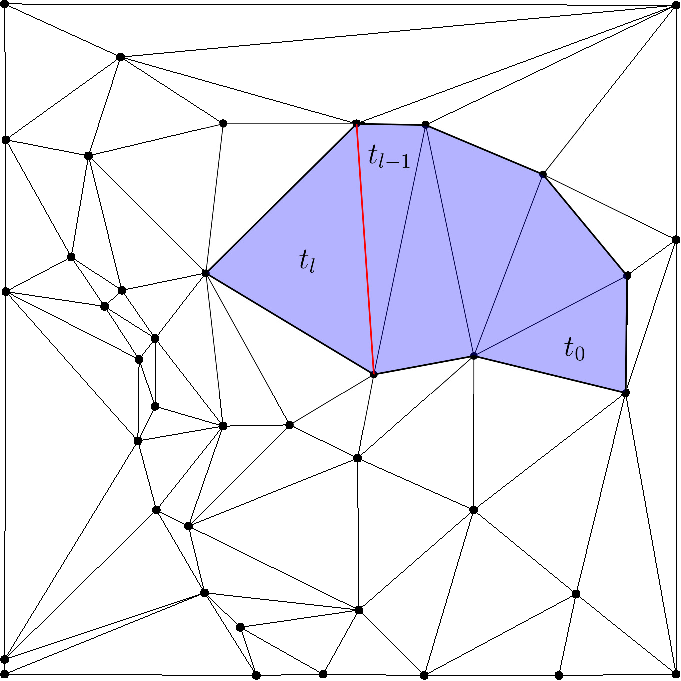
\includegraphics[width=0.3\textwidth]{leppex1}} 
\subfigure[%Lepps with same terminal-edge
]{\label{fig:leppex2}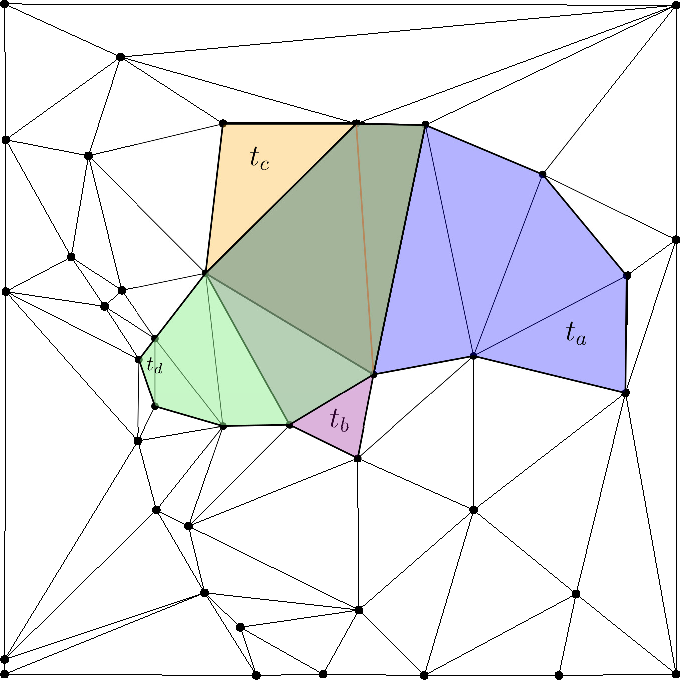
\includegraphics[width=0.3\textwidth]{leppex2}}
\subfigure[%Terminal-edge region
]{\label{fig:leppex3}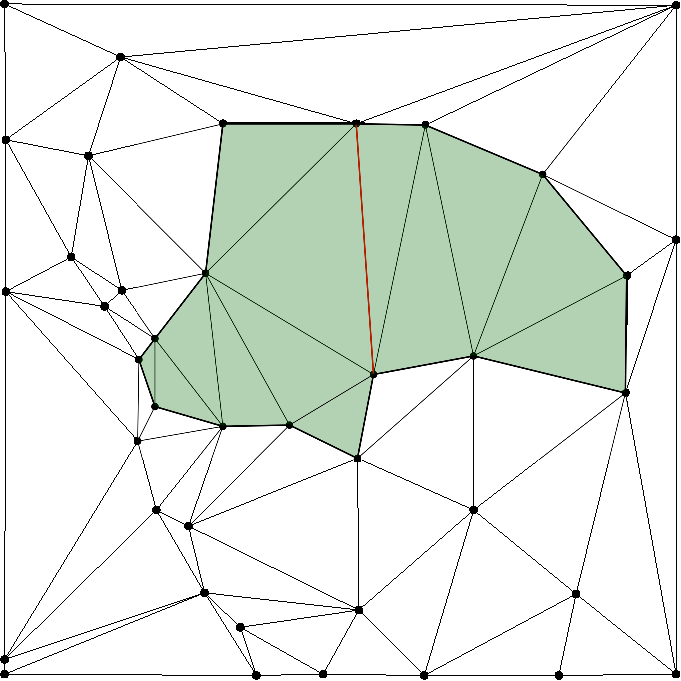
\includegraphics[width=0.3\textwidth]{leppex3}}
\caption{Terminal-edge region. \textbf{(a)} Longest-edge propagation of $t_0$ where the red edge is the terminal-edge. \textbf{(b)} Four Lepps: Lepp($t_a$), Lepp($t_b$), Lepp($t_c$) and Lepp($t_d$), with the same terminal-edge. \textbf{(c)} Terminal-edge region generated by the union of Lepp($t_a$), Lepp($t_b$), Lepp($t_c$) and Lepp($t_d$).}
\label{fig:leppexample} 
\end{figure}

\noindent
A triangle edge can be classified according to its  length inside the two triangles that share it. Therefore, given an edge $e$ and two triangles $t_1$, $t_2$ that share $e$, we can label  $e$ as: 

\begin{itemize}
    \item Terminal-edge~\cite{Rivara97}: $e$ is the longest-edge of $t_1$ and $t_2$.
    \item Frontier-edge~\cite{Ascom209}: $e$ is neither the longest-edge of $t_1$ nor $t_2$. 
    \item Internal-edge:  $e$ is the longest edge of $t_1$ but not of $t_2$ or vice-versa.
    \item Boundary edge: $e$ belongs to one triangle. In the proposed algorithm boundary edges are handled as frontier edges.
\end{itemize}

\noindent
It is worth mentioning that edges of equal length can appear. Therefore, in case there are equilateral  triangles, each edge is chosen arbitrarily as the longest-, the middle- and smallest-edge. When there are isosceles triangles, something similar is done for equal size edges.


\begin{definition}{\textbf{Terminal-edge region~\cite{Ascom209}:}}
\label{d:terminaledgeregion}
A {\em terminal-edge region} $R$ is a region formed by the union of all triangles $t_i$ such that Lepp($t_i$) has the same terminal-edge.  In case the terminal-edge region  is partially delimited by boundary edges the region will be called {\em boundary terminal-edge region}. Fig. \ref{fig:leppexample}(c) shows the terminal-edge region formed by the union of  Lepp($t_a$), Lepp($t_b$), Lepp($t_c$) and Lepp($t_d$). 
\end{definition}


\noindent
We have already used  the concept of terminal-edge region for finding polygonal voids (holes) inside a point set~\cite{HerviasHCF13,Ascom209} and proven some geometric properties. In order to facilitate understanding of the algorithm we are recalling the most important here:

\begin{itemize}
    \item Terminal-edge regions are surrounded by frontier-edges~\cite{Ascom209}.
    \item Terminal-edge regions cover the whole domain without overlapping~\cite{Ascom209,Ojeda2018ANA}.
    \item Terminal-edge-regions might include frontier-edges in their interior. We have called this kind of frontier-edge a \textbf{barrier-edge}~\cite{Ascom209,Ojeda2018ANA}.
  
\end{itemize}
\noindent

%{\bf SERGIO: REVISAR EN EL PAPER SI HAY OTRAS PROPIEDADES UTILES}

%{\bf mencionar que pasa con triangulos equilateros}

\noindent
Let us use Fig. \ref{fig:general_example} to illustrate an example of a partition generated by terminal-edge regions. Fig.~\ref{fig:initialpoinset} shows an input point set; Fig.~\ref{fig:labelsystem} shows the Delaunay triangulation of this point set where terminal-edges are drawn using red dashed lines, internal-edges using black dashed lines and frontier-edges using  solid lines. Fig.~\ref{fig:terminalregion} shows the polygons defined by  terminal-edge regions using a different color, where each polygon is delimited by  frontier edges. It can be noticed that the green polygon is a non-simple polygon because it includes a barrier-edge. \noindent
For simplicity, in the case  $e$ is a domain boundary edge, $e$ will be considered a frontier-edge too (see the edges belonging to the square in Figs. \ref{fig:labelsystem} and \ref{fig:terminalregion}). 

\begin{figure}[h]
\centering     %%% not \center
\subfigure[%Initial point set
]{\label{fig:initialpoinset}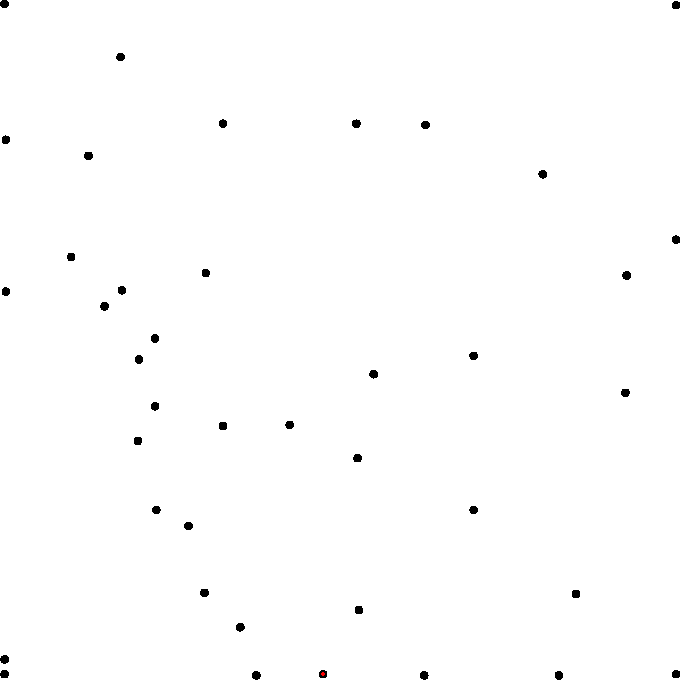
\includegraphics[width=0.3\textwidth]{delaunaypoints}} 
\subfigure[%Delaunay triangulation
]{\label{fig:labelsystem}
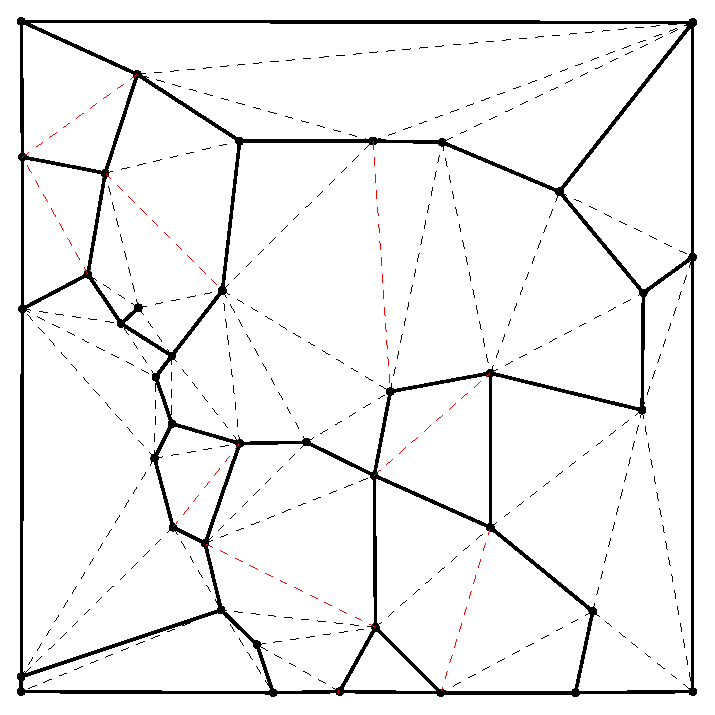
\includegraphics[width=0.3\textwidth]{delaunaylabel}}\subfigure[%Terminal-edge regions
]{\label{fig:terminalregion}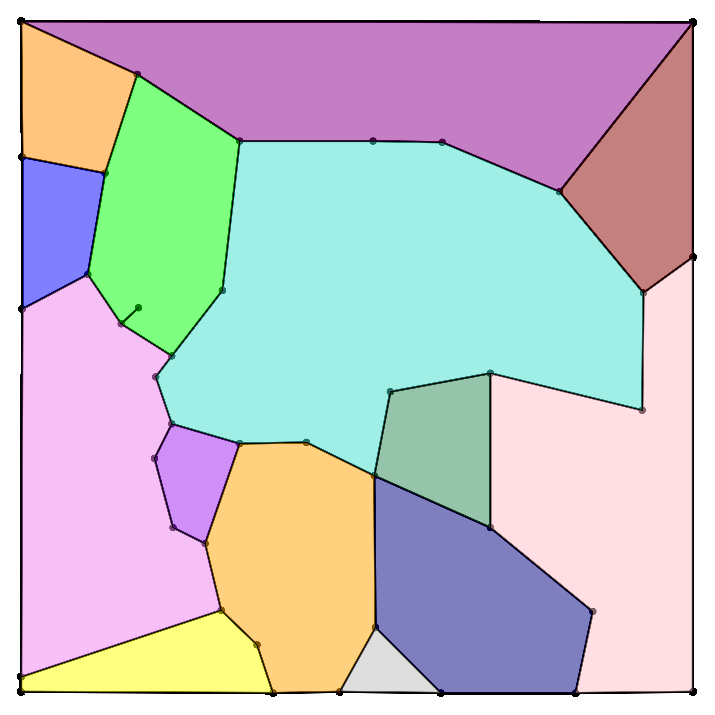
\includegraphics[width=0.3\textwidth]{delaunaylabelcolors}}
\caption{(a) Initial random point set. (b) Delaunay triangulation: Solid lines are frontier-edges, dashed black lines are internal-edges and red dashed lines are terminal-edges. (c) Polygon partition from terminal-edge regions.}
\label{fig:general_example} 
\end{figure}

\subsection{Terminal-edge regions as  polygons}

%\textbf{A esto le falta intro y decir porque es importante nombrarlo}

As we have said in the previous section, terminal-edge regions generate a polygon partition of the domain without overlapping. Depending on the point distribution,  polygons can be simple or  non-simple polygons. Non-simple polygons appear when terminal-edge regions include barrier-edges.  As observed in Fig.~\ref{fig:general_example}, the domain was tessellated into 14 polygons where only the green region is represented by a  non-simple polygon because it includes one barrier-edge. 
%\begin{figure}
%    \centering
%    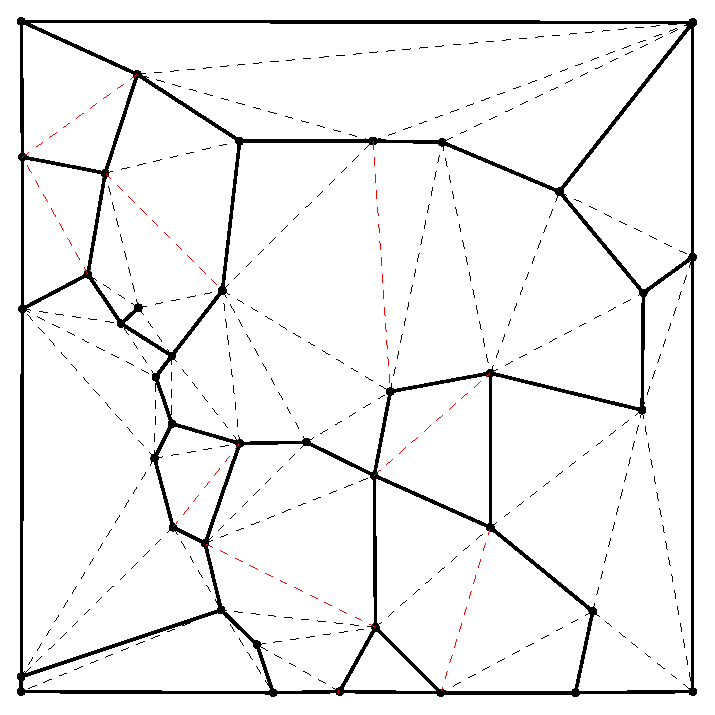
\includegraphics[width=0.5\textwidth]{delaunaylabel}
%    \caption{Terminal-edge regions: Solid lines are frontier-edges, dashed black lines are internal-edges and red dashed edges are terminal-edges.}
%    \label{fig:general_example}
%\end{figure}



  
%\begin{definition}{\textbf{Barrier-edge:}}
%\label{d:barrier-edge}
%A {\em barrier-edge} is a especial kind of frontier-edge: the %triangles that share it belong to the same terminal-edge %region. The barrier-edges generate  non-simple polygon as shown %in Fig. \ref{figs:kindofbarrieredges}.
%\end{definition}

In order to build a conforming polygon tessellation from the partition generated by the terminal-edge regions, non-simple polygons must be divided into simple polygons. That requires the integration of barrier-edges as part of the boundary of new simple polygons.  Since this requirement is part of the meshing algorithm we are proposing in Section~\ref{sec:the_algorithm},  beforehand, we need to introduce some definitions and prove some properties that will sustain the correctness of the algorithm.


\begin{definition}{\textbf{Barrier-edge tip:}}
\label{d:barrier-edge}
A barrier-edge tip in a terminal-edge region $R$ is a barrier-edge endpoint shared by no other barrier-edge/frontier-edge.
%4 nor frontier-edge. See Fig. \ref{figs:kindofbarrieredges}.\\
\end{definition}

%{\bf SERGIO: Marcar los barrier edge tips en la figura y describir mejor cada caso en el texto!!!!}
 
Fig. \ref{figs:kindofbarrieredges} includes  two polygons with barrier-edges; the barrier-edge tips are shown in  green. Fig. \ref{fig:1be} shows a case of a polygon with one barrier-edge tip and Fig. \ref{fig:2be} a case with two barrier-edge tips.
% there is no limit to the maximum number of barrier-edges for a polygon. 
We have observed that each point of the input data is an endpoint of a frontier-edge or barrier-edge. This means that terminal-edge regions have none isolated interior points.
%Barrier-edge tips belong to a barrier-edge.
Theorem~\ref{D:theoreemvertices} demonstrates this property.



\begin{figure}[h]
\centering  
\subfigure[%One barrier-edge and one tip
] {\label{fig:1be}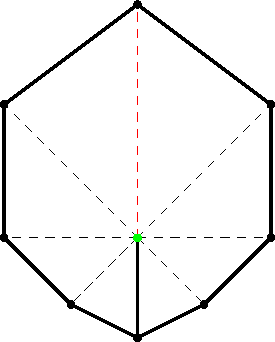
\includegraphics[width=0.15\textwidth, ]{simplebe}}\hspace{2cm}
\subfigure[%Four barrier-edges and two tips tip
]{\label{fig:2be}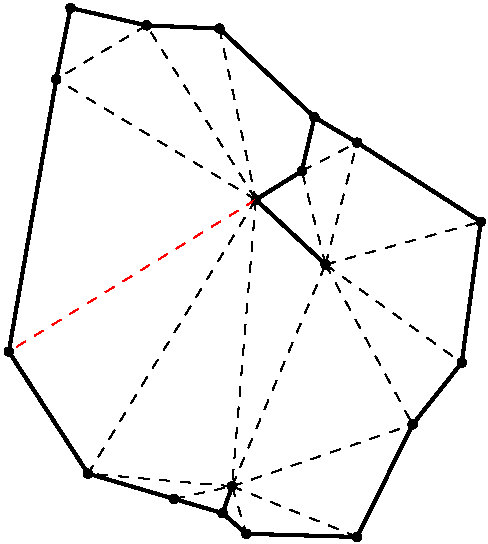
\includegraphics[width=0.15\textwidth, angle =60]{nosimplebe}}\hspace{0.5cm}

\caption{Examples of non-simple polygons. Black lines are frontier-edges, dashed black lines are internal-edges and red edges are terminal-edges. \textbf{(a)} One barrier-edge and one tip \textbf{(b)} Four barrier-edges and two tips tip }
\label{figs:kindofbarrieredges} 
\end{figure}




%\begin{wrapfigure}{l}{0.4\textwidth}

%\centering
%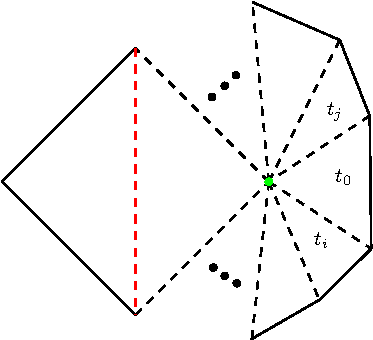
\includegraphics[width=0.9\linewidth]{demostracionlemma2.1} 
%\caption{Green vertex is not part of a frontier-edge.}
%\label{fig:lemmaquitadomingos}
%\end{wrapfigure}
\begin{theorem}
\label{D:theoreemvertices}
Let   $\Omega$ be a triangulation with the set of vertices $V$ in general position. Then, each vertex $v$ is an end-point of at least one  of  the  frontier- or barrier-edges, i.e. there is no isolated interior points (vertices incident only to internal-edges).
\end{theorem}

\begin{proof}: Let $v$ be  a vertex  associated to the terminal-edge region $R$ generated by the terminal-edge $e$ and  $T$ the set of the triangles that share $v$. By contradiction, let us assume that $v$ is an interior point of $R$ as shown  in Fig. \ref{fig:lemmaquitadomingos}. Since the triangles in $T$ are part of $R$, they must share their longest-edge around $v$. 
%with as predecessor  one of the triangles that contains $e$. All edges incidents to $v$ are internal-edges. 
Given that $T$ is finite, there should exist a triangle $t_0$ (see Fig. \ref{fig:lemmaquitadomingos}) that shares their longest-edge with two triangles of $R$ in order to maintain $v$ interior point in $R$. This is not possible because a triangle has just one edge labeled as its  longest-edge. This contradicts our assumption, so $v$ has to be an endpoint of  at least one frontier- or barrier-edge in $R$.  Since triangles in $\Omega$ are distributed into terminal-edge regions without overlap~\cite{Ojeda2018ANA},  isolated points can not exist.
\end{proof}

\begin{figure}[h]
\centering
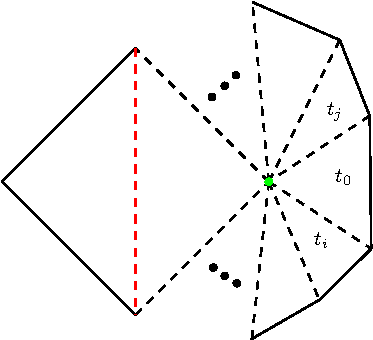
\includegraphics[width=0.25\linewidth]{demostracionlemma2.1} 
\caption{The  vertex in green is an interior point.}
\label{fig:lemmaquitadomingos}    
\end{figure}


It is worth mentioning Theorem \ref{D:theoreemvertices} guarantees that  the initial points used to represent the geometric domain and the ones inside the domain to fulfill point density requirements  are vertices delimiting one or more polygons. Moreover, each  internal-edge is a diagonal of one polygon. Therefore,  interior-edges that contain barrier-edge tips as endpoints  can be used to split a non-simple polygon into simple polygons.

%Note that if the input points are not in general position, the following degenerate case might occur. Let  $v$ be an input point  and $T$ the set of triangles incident to $v$. If all triangles in $T$ are equilateral, it may happen that the algorithm labels each edge $e$ sharing $v$ as the longest-edge in only one of the triangles that share $e$. Then all edges that share $v$ are internal-edges; this case generates a region $R$ with no terminal-edge. This rare case can be solved  by  assigning one edge with  $v$ as endpoint as longest-edge in  the two triangles that share it. In this way, $R$ is now a terminal-edge region.

Note that if the input points are not in general position,  a region without a terminal-edge might appear. This  degenerate region $R$ occur when the algorithm  labels all edges that share a vertex $v$ as internal-edges. This case might happen 
%For example: Let  $v$ be an input point  and $T$ the set of triangles incident to $v$. 
if all triangles in $R$ are equilateral and the algorithm labels each edge $e$ sharing $v$ as the longest-edge in only one of the triangles that share $e$. Then all edges that share $v$ are internal-edges. This rare kind of case can be solved  by  assigning one edge with  $v$ as endpoint as longest-edge in  the two triangles that share it. In this way, $R$ is now a terminal-edge region.


\section{The algorithm}
\label{sec:the_algorithm}

%The algorithm receives as input a Constrained Delaunay triangulation $CTD(\Omega)$ and generates as output a polygonal mesh.  Algorithm consists in three main steps:

In this section, we describe  the main steps of the proposed algorithm, its computational cost  and the data structure used for its implementation.
The algorithm receives an initial triangulation as input, that can be generated by any known triangulator. The triangulation can be Delaunay or not, but we are using Delaunay triangulations because, several polygons of the mesh keep some angles of the triangles of the input triangulation. Since a Delaunay triangulation maximizes the minimum angle over all the possible triangulations for a point set, this angle will be a lower bound for the minimum angle of the generated polygonal mesh.
%\textcolor{blue}{ as Delaunay triangulation is the triangulation with the maximal angles, then the resulting mesh has the maximal angles too. 

There are  several correct and robust triangulators such as Detri2~\cite{Detri2} and Triangle~\cite{triangle2d} available for free.  We are using Detri2 \cite{Detri2} to generate the constrained Delaunay triangulation needed as initial mesh. The whole process applied to the initial triangulation is divided in next three phases:


\begin{enumerate}[label=\roman*)]
    \item Label phase: Each edge is labeled as  longest-, terminal- or frontier-edges to  build terminal-edge regions. The algorithm also labels one  triangle in each terminal-edge region as seed triangle used in the next phase to build each polygon.
    \item Traversal phase: Generation of polygons from seed triangles. In this phase the frontier-edge vertices of a terminal-edge region are stored in counter-clock-wise (ccw) order to  build a polygon. Non-simple polygons generated in this phase are sent to the reparation phase.
    \item Reparation phase: Polygons with barrier-edges are partitioned into simple polygons.
\end{enumerate}


\subsection{Data structures}
\label{sec:datastructrue}
%\textbf{Mover la estructura de datos dentro del algoritmo, ponerlo depsués del análisis de complejidad}
In this subsection we describe the data structures used in our implementation. We have decided to use an indexed data structure with adjacencies as  described in \cite{MeshDatastructSurvey}.  The purpose of the following representation is to have an easy and compact way to travel through all the faces of the triangulation and, in an implicit way, by using a special order in the representation, to access their edges and neighbor triangles in ccw. 

The triangulation is represented using three one-dimensional arrays for the vertices, triangles and neighbor triangles, respectively.  %The data structures and the operations to access the values are very similar to the ones used by Detri2 \cite{Detri2}, \textbf{Poner que se puede conseguir en qhull con  Fv Fn Fa QJ y en triangle por defecto el output de los neigh file es este.}
Vertices are stored in pairs $(x,y)$, where each two consecutive elements of the Vertex array are the coordinates $x$ and $y$ of a point. The Triangle array is a set of indices to the Vertex array. Each 3 consecutive values is a triangle. Since the algorithm needs to know the neighbor through each triangle edge, the Neighbor array  stores the three indices of the neighbor triangles of  triangle $i$ at the locations $3i + 0$, $3i + 1$, $3i + 2$. %\textcolor{blue}{with 0,1,2 the indices of the edges of $i$.}

To facilitate the implementation of the algorithm, vertex indices in the Triangle array are ordered  in such a manner that is easy to find out which is the neighbor triangle through  each triangle edge. Fig. \ref{figs:data_and_triangle}(a) illustrates the connections of each array element. The first two point indices $3i+0$, $3i+1$ in the Triangle array is an edge of triangle $i$ and this edge is shared with the triangle stored in the position $3i+2$ of the Neighbor array; the triangle edge defined by $3i+1$, $3i+2$ in the Triangle array is shared with the triangle stored  in $3i+0$ in the Neighbor array and the triangle edge $3i+2$, $3i+0$ in the Triangle array with the triangle stored at $3i+1$ in Neighbor array. Triangle edges are stored implicitly: the green edge in Fig. \ref{figs:data_and_triangle}(b) corresponds to the first one,  the  red  edge is  the second one and the blue  the third one.  These neighborhood relations can currently be generated as output by several tools such as  Qhull \cite{qhull}, Triangle \cite{triangle2d} and Detri2qt \cite{Detri2}.

\begin{figure}
\centering     %%% not \center
\subfigure[]{\label{fig:datastruc}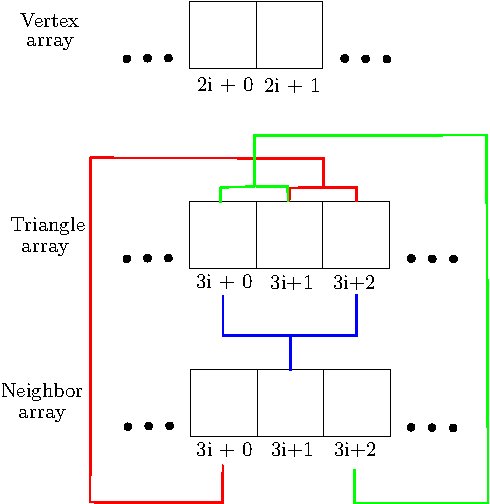
\includegraphics[width=0.3\textwidth]{TriangleDatastruct}}\hspace{2cm}
\subfigure[]{\label{fig:datastructriangle}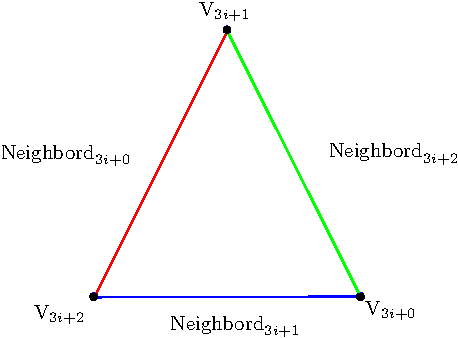
\includegraphics[width=0.3\textwidth]{triagleccw}}
\caption{Data structure:  \textbf{(a)} Relation between the  vertex indices in the Triangle array and the triangle indices in the Neighbor array. \textbf{(b)} Triangle information stored  in the data structure shown in (a)
.}
\label{figs:data_and_triangle} 
\end{figure}







%a integer list of length equal to the number of terminal-edges,  (they are store in label phase) and  % To simulate splits of polygon, the algorithm search the initial point and the endpoint of the edge to add in the array of the polygon and generate two polygons to calculate the optimal area as is show in Fig. \ref{fig:b_data_poly}. 


The final mesh composed of simple polygons is also stored in  one array, where each polygon includes first its number of vertices and then the vertex indices in ccw  as shown in Fig. \ref{fig:meshdatastruct}. 

Data structures to store additional information needed only in one of the steps of the algorithm are mentioned in the respective subsection. It is worth mentioning here the representation of non-simple polygons since this information is used in two phases. Fig. \ref{fig:poly_array_representation}  shows an example of a polygon with two barrier edge tips. This kind of polygon is stored in an index array  in the same way as a simple polygon in order ccw, and it is recognized as non-simple because there are repeated vertex indices. The same occurs with the seed list $L$, which is initialized in the Label phase with one triangle index per each terminal-edge region, and used in the Traversal phase to build polygons.  

\begin{figure}[]
    \centering
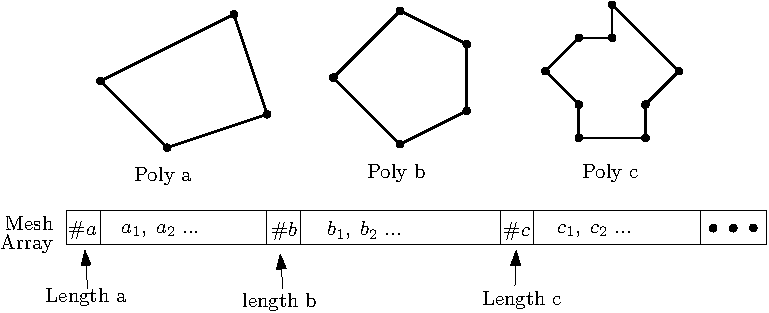
\includegraphics[width=0.6\textwidth]{meshdatastruct}
    \caption{Mesh array with three polygons.} 
    \label{fig:meshdatastruct}
\end{figure}


\begin{figure}
\centering     %%% not \center
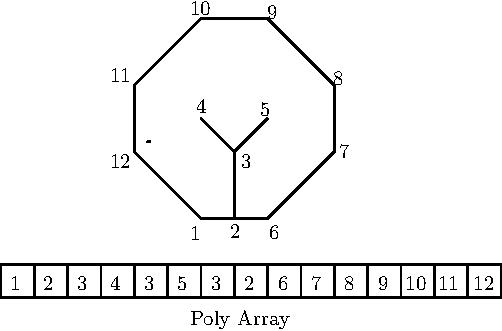
\includegraphics[width=0.4\textwidth]{polyarray} 
%\subfigure[Data structure]{\label{fig:b_data_poly}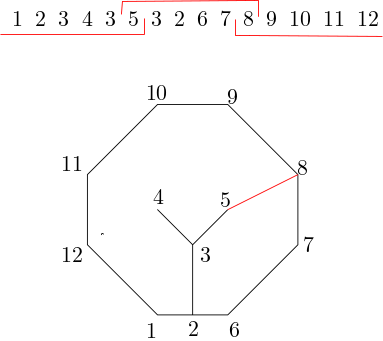
\includegraphics[width=0.31\textwidth]{datastructure_split2}}
%\subfigure[Data structure]{\label{fig:c_data_poly}\includesvg[width=0.3\textwidth]{datastructure_split3.svg}}
\caption{Representation of a  non-simple polygon as a set of vertex indices in ccw. Sequences $3 - 4 - 3$ and $3 - 5 - 3$ indicate the existence of barrier-edge tips.}%\textbf{(b)} Simulation of addition of an edge to calculate the optimal distance.}
\label{fig:poly_array_representation} 
\end{figure}


%Let be $R$ the terminal-edge region set and $B$ the set of terminal-edge regions with barrier-edge tips ($B \in R$), $\sum b_i$ the sum of all barrier-edge tips in $B$, the seed list has size $R$ and the mesh array has a max size of $\#R + \#B + \sum b_i)$ of elements.

%\textcolor{red}{As $R$ is a subset of elements generated from the face of a triangulation, and the total number of triangles is $O(n)$, then the total cost of memory of the algorithm is $O(n)$.}



%To the reparation phase a recursive function had been chosen to split polygons (split a polygon in two, and those two split them again until removing all barrier-edge tips), but to optimise the use of memory a open hash table $H$ was use. This table is an array of arbitrary length with pointers to linked list where save the seed triangles uses to generate the new polygons where each element is added to the begin of the linked list and each search operation has a delete operation inside to remove already use triangles.


\subsection{Label Phase}
\label{subsec:Labelpohase}

The goal of the Label phase  is to find  frontier-edges, terminal-edges and seed  triangles to build polygons in the next phase. The pseudo-code of this process is shown in Algorithm \ref{algo:labelphase}.
The algorithm first cycles over each triangle  of the initial triangulation (line \ref{algolabel:TriangleIteration}) to compute which edge is the longest-edge and stores this edge index (one per each triangle)  in a temporal array of size equal to the number of triangles; in the case of equilateral and isosceles triangles, the algorithm assigns  randomly a size order to the equal length edges  to avoid having a triangle that belongs to two terminal-edge regions at the same time. % \cite{Ojeda2018ANA, jojeda}.

%\textcolor{red}{ in the data structure, this means mark the neighbor as $-1$, for example, in Fig. \ref{figs:data_and_triangle}, to label red edge as frontier edge, $Neighbord_{3i+0}$ must change its value by $-1$.}

Afterward, the algorithm does a second iteration over the edges (line \ref{algolabel:Edgeiteration}). In case  an edge $e$ is not the longest-edge of any of the two triangles that share it (line \ref{algolabel:label}), $e$ is labeled as a frontier-edge. In case $e$ is a terminal-edge (line \ref{algolabel:seedtrianglelabel}), the algorithm stores the  smallest index of the triangles that share it in the Seed list $L$. In the case of a boundary terminal-edge, the index of the unique triangle is  stored. 

\begin{figure}[h]
\centering     %%% not \center
\subfigure[%Delaunay Triangulation
]{\label{fig:delunolabel}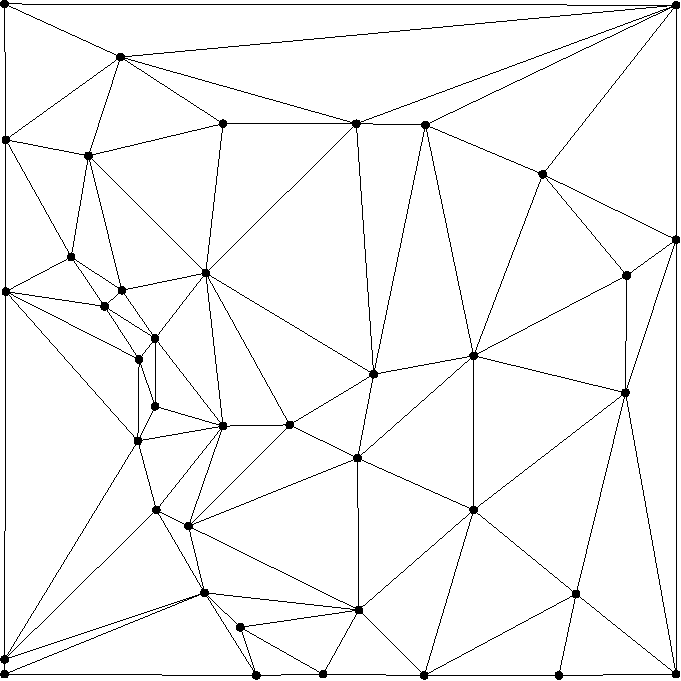
\includegraphics[width=0.4\textwidth]{delunolabel}} \hspace{0.5cm} 
\subfigure[%Triangulation after applying the label phase
]{\label{fig:Labelphaseafter}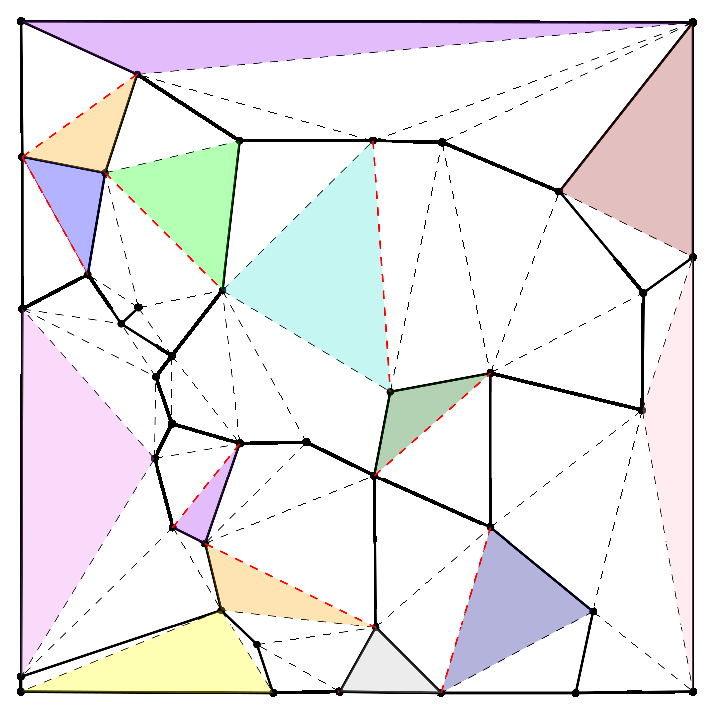
\includegraphics[width=0.4\textwidth]{labelandseedcolors}}
\caption{Label phase: (a) Input Delaunay triangulation. (b) Solid lines are the frontier-edges, dashed lines are the internal-edges and colorful triangles are seed triangles. }
\label{figs:label_phase} 
\end{figure}

The final result of this step is shown in Fig. \ref{figs:label_phase}(b). The colorful triangles are the seeds used in the next phase to generate the polygons. It can also be  observed that terminal-edge regions are  delimited by frontier-edges. 
%those edges are the edges of the final mesh.

\begin{algorithm}
    \caption{Label phase}\label{algo:labelphase}
    \begin{algorithmic}[1]
    \Require Initial Triangulation $\Omega$
    \Ensure Labeled edges and seed triangles of $\Omega$ 
    \ForAll{triangle $t_i$ in $\Omega$} \label{algolabel:TriangleIteration}
        \State Label the longest-edge of $t_i$
    \EndFor
    \ForAll{edge $e_i$ in $\Omega$} \label{algolabel:Edgeiteration}
        \State Be $t_1$ and $t_2$ triangles that share $e_i$
        \If{$e_i$ neither the longest-edge of $t_1$ nor $t_2$ or $e_i$ is border-edge} \label{algolabel:label}
            \State Label $e$ as frontier-edge
        \EndIf    
        \If{$e_i$ is terminal-edge or border terminal-edge} \label{algolabel:seedtrianglelabel}
            \State Choose one triangle sharing $e_i$ and store its index in the Seed list $L$
        \EndIf    
    \EndFor
    \end{algorithmic}
\end{algorithm}

%describir el etiquedado
%hacer un dibujo ql
%tula

\subsection{Traversal Phase}
\label{subsec:Travelpohase}

In this phase, polygons are built and represented as a closed polyline as shown in Fig. \ref{fig:poly_array_representation}. The main idea behind this phase is to travel through neighbor triangles, neighbors by  internal-edges inside a terminal-edge region and save their frontier-edges as edges of the new polygon $P$ in ccw. For this reason, the algorithm uses each triangle $t$ inserted in the Seed list $L$ as the starting triangle to build each polygon. The pseudo-code of this phase is shown in Algorithm \ref{algo:travelphase}. 
%For this purpose, the algorithm  uses each triangle $t$ in the seed list created, in the previous phase, as the starting triangle to build each polygon. %Note that every triangle can be used to generate a polygon, but we use one triangle neighbor to a terminal-edge to avoid generating the same polygon twice.

From line \ref{algotravel:init} until line \ref{algotravel:initend}, the algorithm gets the first triangle $t$ from the Seed list and  initializes the variables according to  the number of frontier-edges that $t$ has.  In case $t$ has 3 frontier-edge edges, $t$ is stored in the polygon $P$ as a whole polygon. In case $t$ has less than $3$ frontier-edges, their endpoints are saved as the first points of $P$ in ccw. In addition, the first vertex  of $P$ and $t$ are saved in $v_{init}$ and $t_{init}$, respectively, to check when the polygon boundary is ready. It is also necessary to store the last added vertex  in $P$ in $v_{end}$ to look for the e endpoint to be added. In case $t$ has no frontier-edge (Line \ref{algotravel:initial0edgescase}), the algorithm saves any vertex of $t$ as $v_{init}$ and $v_{end}$, and  $t$ in $t_{init}$. In the end, all vertices of $t$ will be part of polygon boundary; then it does not matter which one is taken as the initial point. After the initialization, the algorithm travels to the next internal-edge neighboring triangle $t'$ that shares $v_{end}$ with $t$. Three cases for $t'$ must be  considered:

%It is also necessary to keep  track of the  last  added vertex in $P$ ($v_{end}$) to look for the next frontier-edge endpoint to be added.


%Let be $t$ a triangle of the seed list and $P$ a temporary array to store a polygon, if $t$ has 3 frontier-edges (line \ref{algotravel:initial3edgescase}), then $t$ is saved as a polygon in $P$, and the algorithm goes to the next triangle in the seed list, else, if the algorithm has three or two frontier-edges (lines \ref{algotravel:initial2edgescase} and \ref{algotravel:initial1edgescase}), its stores the tree or two continuous endpoints  of the edges of $t$ labeled as frontier-edge in $P$ in ccw, saves $t$ as a initial triangle, choose the first stored endpoint $v_{init}$ in $P$ as initial vertex (by lemma \ref{D:theoreemvertices} each vertex of a terminal-edge region is part of a frontier-edge) and the last stored endpoint $v_{end}$ in $P$. \textcolor{red}{If $t$ has no frontier-edges (line \ref{algotravel:initial0edgescase}), then the algorithm defines one vertex of $t$ as $v_{init}$ and $v_{end}$ and saves $t$ as initial triangle.} After, the algorithm travels to the next neighbor triangle $t'$ in ccw that have $v_{end}$ as vertex. There are three cases for $t'$:

%For this purpose, the algorithm  uses each triangle $t$ in the seed list created in the previous phase as the starting triangle to built each polygon. 
%The algorithm stores the frontier-edges of $t$ (if it has one), chooses one frontier-edge vertex as an initial point $v_{init}$ and the other as an endpoint $v_{end}$ and travel  through the next adjacent triangle $t'$ searching for new frontier edges. 
%The algorithm considers three following  cases for $t'$:


%decir como se inicia el viaje, con t triangulo inicial y t' el nuevo triangulo, con tres frontier edge es poligono.

%agregar el caso cuando por problemas de prescion no hay semilla



\begin{enumerate}[label=\roman*)]
    %comparte un arco con $t$, explicar con t' y t el anterior, t tiene un arco frontera y es endpoint de t', t' 
    \item Line \ref{algotravel:twoedgecase}: The triangle $t'$ has just  one frontier-edge $e$ and this edge contains $v_{end}$. Then $e$ is stored in $P$ and $v_{end}$ is updated with the other $e$ endpoint. The next triangle $t'$ is the non-visited internal-edge neighbor triangle that contains the new $v_{end}$. % Then $t'$ shares an frontier-edge with the last triangle visited (where the last endpoint $v_{end}$ come from), and a frontier edge with a triangle that can be visited, the new $t'$ is that last no visited triangle.
    
    \item Line \ref{algotravel:oneedgecase}: The triangle $t'$ is an ear triangle (a triangle with 2 frontier-edges). In this case, both edges are stored in ccw in $P$ and $v_{end}$ is updated with last stored endpoint. The previously visited triangle is the new $t'$ because the other two triangles are neighbor by frontier-edges (i.e., they belong to other terminal-edge regions).
    
    \item Line \ref{algotravel:noedgecase}: The triangle $t'$ has no frontier-edge. $t'$ shares an internal-edge with the last visited triangle and with the other two neighbor triangles that can be visited. Just one of these two triangles contains the endpoint $v_{end}$ as vertex, so that triangle is the new $t'$. 
    %This case can occur when a barrier-edge is found, when a triangle is between two ear triangles or when the algorithm surrounds an ear triangle of another terminal-edge region.
\end{enumerate}

%The Travel phase ends when $v_{end}$ reaches the initial point $v_{init}$ and the initial triangle $t_{init}$ is the same as $t'$ (line \ref{algotravel:end}).
% Experiments showed that both conditions are necessary, the first one due to a triangle can be visited multiple times in flat polygons and the second one due to barrier-edges can be omitted if only the first condition is used. An example of this phase is shown in Fig. \ref{fig:travelphase}.

\begin{figure}[h]
    \centering
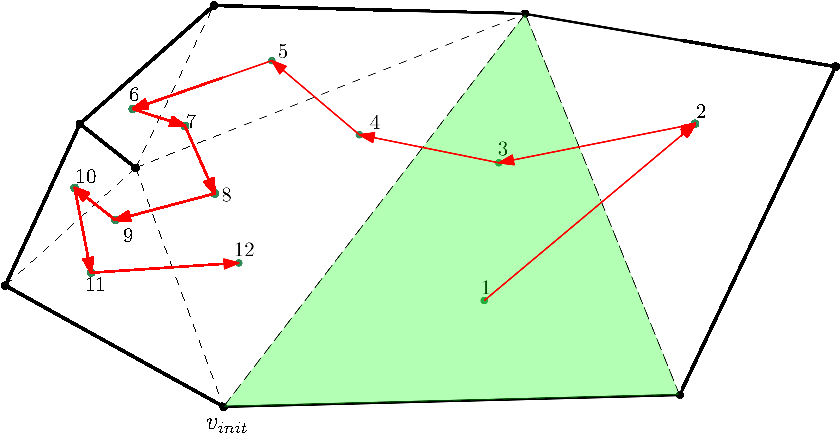
\includegraphics[width=0.5\textwidth]{travelphase4}

    \caption{Traversal phase. The green triangle is the seed triangle of this terminal-edge region. The labels indicate in which order  each triangle was visited. } 
    \label{fig:travelphase}
\end{figure}



\begin{algorithm}
    \caption{Polygon construction}\label{algo:travelphase}
    \begin{algorithmic}[1]
    \Require Seed triangle $t$ of a terminal-edge region
    \Ensure Arbitrary shape polygon
    %\State Polygon $\leftarrow$ $\emptyset$, Mesh $\leftarrow$ $\emptyset$ 
    %\ForAll{triangle $t$ in seed list}
    \State Polygon $\leftarrow$ $\emptyset$ \label{algotravel:init}
        \If{ $t$ has $3$ frontier-edges $e_1$, $e_2$ and $e_3$} \label{algotravel:initial3edgescase}
            \State \Return Polygon $\leftarrow$ $e_1 \cup	 e_2 \cup	e_3$
        \ElsIf{ $t$ has $2$ frontier-edges $e_1$ and $e_2$} \label{algotravel:initial2edgescase}
            \State $v_{init} \leftarrow e_1.v_{first}$,  $v_{end} \leftarrow e_2.v_{second}$
            \State Polygon $\leftarrow$ $e_1 \cup e_2$
        \ElsIf{ $t$ has $1$ frontier-edge $e_1$} \label{algotravel:initial1edgescase}
            \State $v_{init} \leftarrow e_1.v_{first}$, $v_{end} \leftarrow e_1.v_{second}$
            \State Polygon $\leftarrow$ $e_1$
        \ElsIf{$t$ has no frontier-edges} \label{algotravel:initial0edgescase}
            \State $v_{init}, v_{end} \leftarrow t.v_{0}$
        \EndIf    
    %\State $t_{init} \leftarrow$  $t$  by one edge that shares 
    \State $t' \leftarrow$ internal-edge neighbor triangle of $t'$ that shares $v_{end}$  \label{algotravel:initend}
    \While {$v_{init} \not= v_{end}$ and $t' \not= t_{init}
    $} \label{algotravel:end}
        \If{ $t'$ has $2$ frontier-edges $e_1$ and $e_2$ with $e_1$ continuous to $v_{end}$} \label{algotravel:twoedgecase}
            \State Polygon $\leftarrow$ Polygon $\cup$ $e_1 \cup e_2$
            \State $v_{end} \leftarrow e_2.v_{second}$
            \State $t' \leftarrow$ last visited triangle
        \ElsIf{$t'$ has $1$ frontier-edge $e_1$ continuous to $v_{end}$} \label{algotravel:oneedgecase}
            \State $v_{end} \leftarrow e_1.v_{second}$
            \State Polygon $\leftarrow$ Polygon $\cup$ $e_1$
            \State $t' \leftarrow$ internal-edge neighbor triangle not visited in previous iteration that contains $v_{end}$
        \Else \label{algotravel:noedgecase}
            \State $t' \leftarrow$ internal-edge neighbor triangle in ccw that contains $v_{end}$
        \EndIf 
    \EndWhile
    %\If{Polygon has barrier-edge tips}
    %    \State Send to reparation phase
    %\EndIf
    %\State Save Polygon(s) in Mesh  
    %\EndFor
    %\State \Return Mesh
    \State \Return Polygon $P$
    \end{algorithmic}
\end{algorithm}

Algorithm~\ref{algo:travelphase} is applied to each seed triangle and returns a polygon $P$. Note that triangles with no frontier-edges are visited 3 times, with one frontier-edge two times and with two frontier-edges one time; this is demostrated in Lemma \ref{l:lemmatravelphase}. In case $P$ has barrier-edge tips, the algorithm described in Section~\ref{subsec:nonsimplereparation} is used to divide it into simple-polygons. A non-simple polygon can be easily detected by just checking the repetition of consecutive vertices in $P$: given three consecutive vertices of $P$, $v_i$, $v_j$ and $v_k$, if $v_i$ and $v_k$ are equal, then $v_j$ is a barrier-edge tip. In case $P$ does not have barrier-edge tips,  the polygon is saved as part of the mesh in the Mesh array.


\begin{lemma}{Each triangle is visited at most $3$ times during the polygon construction from a terminal-edge region.} \label{l:lemmatravelphase}
\end{lemma}

\begin{proof}: By construction,  the algorithm can only  visit triangles through their internal edges. The worst case  is when a triangle has 3 internal edges (no frontier-edges); then this triangle is visited once per internal edge, i.e. 3 times. In case of 2-internal edges, the triangle is visited 2 times and in case of 1 internal-edge just 1 time.

%Note as each vertex in a terminal-edge region $R$ is part of a frontier-edge (Theorem \ref{D:theoreemvertices}), each internal-edge acts as separation between sub-regions $r_i$ of $R$. Be $t$ a triangle of $R$, each internal-edge of $t$ is connected to a subregion $r_i$ and the algorithm uses $t$ as bridge to get the frontier-edge of those subregions.

%Therefore, the most visited triangle, is a triangle with 3 internal-edges, in that case, $t$ is connected $t$ to the subregions $r_1, r_2, r_3$. If $r_1$ is the subregion with the seed triangle, the algorithms travels from $r_1$ to $r_2$, after, travels from $r_2$ to $r_3$ and goes back from $r_3$ to $r_1$, as the exit condition is in $r_1$ the algorithm does not goes back $t$ and $t$ is visited $3$ times. As there is not a triangle with $4$ internal-edges, then the maximum number of times that a triangle is visited during the travel phase is $3$.
\end{proof}

%\begin{proof}
%{\color{red} Note as each vertex in a terminal-edge region $R$ is part of a frontier-edge (lemma \ref{D:theoreemvertices}), each internal-edge act as separation between sub-regions $r_i$ of $R$, the algorithms uses those internal-edge to change between subregions and gets their frontier-edge as part of $P$. Be $t$ an arbitrary triangle of $R$, there is four cases to the number of times that the algorithm visits $t$:

%\begin{itemize}
    %\item If $t$ has 3 frontier-edges, the algorithm does not need to do a travel, it just store all frontier-edge of $t$ as part of $P$.
   % \item If $t$ has 2 frontier-edges, 1 internal-edge $e_1$ that connect $t$ to the subregion $r_i$. Then the algorithms enters to $t$ by $e_1$ from $r_1$, stores the 2 frontier-edge in $P$, and back to $r_1$ using $e_1$, as the exit condition is in $r_1$ the algorithm does not back to $t$ and $t$ was visits one time.
  %  \item If $t$ has 1 frontier-edge, 2 internal-edges $e_1$ and $e_2$, in ccw, and both are connected to two subregions $r_1$ and $r_2$, respectively. The algorithm enters from $r_1$ to $t$ using $e_1$ and out of $t$ to $r_2$ using $e_2$, after stores all frontier-edges of $r_2$, the algorithm backs to $t$ by $e_2$ and exit to $r_1$ using $e_1$. In $r_1$ the algorithm gets the exit condition and it does not back to $t$. Depending of the position of the frontier-edge the algorithm stores their frontier-edge in one of the two visit to $t$.
 %   \item If $t$ has no frontier-edges, 3 internal-edge $e_1, e_2, e_3$, in ccw, that connect $t$ to the subregions $r_1, r_2, r_3$, respectively. In order to store the frontier-edges of $r_1$, $r_2$ and $r_3$, the algorithm uses the internal-edges of $t$ and visits $t$ 3 times, one to travel from $r_1$ to $r_2$, other to travel to $r_3$ from $r_2$ and the last one to back to $r_1$ from $r_3$. As the exit condition is in $r_1$ the algorithm does not back $t$.

%\end{itemize}

%The cases are the same for when $t$ is a seed triangle, and therefore, $t$ is the exit condition. As in all four cases the algorithm visits at most $3$ times $t$, then each triangle is visited at the most 3 times during the Polygon construction.  }
%\end{proof}

%Poner aquí imagen de los tres casos mñn uwu

\subsection{Non-simple polygon reparation}
\label{subsec:nonsimplereparation}

As previously mentioned, some polygons generated in the Traversal phase are non-simple. In this section, we describe an algorithm to divide non-simple polygons into simple-ones by using internal-edges containing barrier-edge tips as one of their end-points. 
%\textcolor{red}{as vertices of the input triangulation are information of the geometry, we create this method instead of just delete the barrier-edges of the polygon.}%\textcolor{red}{this is made to maintain the same vertices of the input triangulation in the outputting Polylla mesh, }. 
Notice that a simple strategy could just be to remove barrier-edges and keep as polygon boundary only the frontier-edges. However, this approach would require to delete barrier-edge endpoints, which are vertices defined/inserted in  the initial triangulation by the user/triangulation tool. We assume that all points are important. That is why, we propose  a method to repair non-simple  polygons without removing initial vertices.

The reparation process works similarly to the Label and Traversal phases but inside a non-simple polygon $P$. In short, the algorithm labels so many internal edges as frontier-edges until all barrier-edge tips are part of a polygon boundary and stores one seed triangle per each new polygon in a new Seed list $L_p$. After, those triangles are used as seed to generate the new polygons with the Algorithm \ref{algo:travelphase}. The internal-edges chosen to be new frontier edges are the ones that contribute to generate polygons of similar size.

The reparation algorithm is shown in Algorithm \ref{algo:reparationphase}. For each barrier-edge tip $b_i$ in a polygon $P$ (line \ref{algorepa:foreachbet}), the algorithm computes first $deg(b_i)$, which is the number of incident internal-edges to $b_i$ inside the terminal-edge region. To facilitate this calculation the algorithm uses an auxiliary array that associates to each vertex a triangle. If $deg(b_i)$ is odd then the algorithm labels the middle edge as frontier-edge; otherwise, the algorithm chooses any of the two middle edges as a new frontier-edge. In both cases, the two triangles that share the new frontier-edge are saved in the seed list $L_p$. From line~\ref{algorepa:foreachseedtriangle} to line ~\ref{algorepa:removeseeds}, each new simple polygon is built. A Bit array $A$, of size equal to the number of triangles of the input triangulation is used to avoid the generation of the same polygon more than once. The insertion of one or more seed triangles of the same new polygon in the seed list $L_p$ occurs when a terminal-edge region contains more than one barrier-edge tip. Each seed triangle stored in $L_p$ is set to 1 in $A$; the others are 0. When a polygon is built, each used triangle is set to $0$ in $A$. Fig. \ref{fig:betosplit} shows an example of a non-simple polygon with three barrier-edge tips (vertices in green color). Fig. \ref{fig:besplited} shows the internal-edges converted in new frontier-edges to delimit the new simple polygons and the six seed triangles stored in $L_p$.  Fig. \ref{fig:benewpolygons} shows the four new polygons after the split and the seed triangles used to generate them.

It is worth mentioning that the number of polygons generated after the split is at  most $(\lvert B\rvert + 1)$, with $\lvert B\rvert $ the number of barrier-edge tips in a polygon $P$. 


\begin{lemma} \label{lemma:degReparation}
Let   $\Omega$ be the input triangulation and $B$ the set of barrier edge tips in the polygon $P$. In the computation of $deg(b_i)$,   $\forall b_i, b_i \in B$, each triangle $t$ inside the terminal-edge region that generated $P$ can be visited at most 3 times.
\end{lemma}
\begin{proof}: By construction  
 if a triangle $t$ is not incident to a barrier-edge tip $b_i$, Algorithm~\ref{algo:reparationphase} does not  visit $t$ during the computation of  $deg(b_i)$. If $t$ contains as vertex one, two or three barrier-edge tips, then $t$ is visited one time per each barrier-edge tip. Since $t$ has at most   $3$ barrier-edge tips then $t$ is visited in the worst case $3$ times for the computation of $deg(b_i)$.
\end{proof}


%As we have said in the previous section, the generated polygons might be non-simple; this is the fact when they contain barrier-edges tips. In this section, we describe an algorithm to \textcolor{red}{repair} non-simple polygons into simple-ones by using internal-edges of the initial triangulation that contain barrier-edge tips as one of their end-points. The algorithm exploits Lemma \ref{D:theoreemvertices} which proofs that all input vertices are  end-points of at least one  frontier-edge/barrier-edge. Then by labeling an internal-edge as frontier-edge, any polygon can be divided into two new polygons. Moreover if the internal-edge has one barrier-edge tip as one of its end-points, this barrier-edge is now part of a new polygon boundary. The pseudo-code of this process is shown in Algorithm \ref{algo:reparationphase}.

%The reparation process  works similar to the Label  and Travel phases but inside a non-simple polygon $P$. So first the algorithm labels so many internal edges as frontier-edges until all barrier-edge tips are part of a polygon boundary and \textcolor{pink}{stores one seed triangle per each new polygon in a new Seed list $L_p$}. The  internal-edge chosen to be new frontier edges are the ones  that contributes to generate polygons of similar size. In order to do so, for each barrier-edge tip $b_i$ in a polygon $P$ (line \ref{algorepa:foreachbet}), the algorithm computes first  $deg(b_i)$, the number of incident internal-edges to $b_i$ inside the terminal-edge region. If $deg(b_i)$ is odd then the algorithm labels the middle edge as frontier-edge; otherwise the algorithm chooses any of the two middle edges as a new frontier-edge. In both cases, the two triangles that share the new frontier-edge are saved in the seed list $L_P$. From line~\ref{algorepa:foreachseedtriangle} to line ~\ref{algorepa:removeseeds}, each new simple polygon is built. A Bit array $A$, of size equal to the number of triangles of the input triangulation, is used to avoid the generation of the same polygon more than once.  \textcolor{red}{The insertion of two seed or more seed triangles, of the same new polygon, in the seed list $L_p$ occurs when a terminal-edge region contains more that one barrier-edge tip.} Each seed triangle stored in $L_p$ is set to 1 in $A$; the others are 0. When a polygon is build, each used triangle is set to $0$ in $A$. Fig. \ref{fig:betosplit} shows an example of a non-simple polygon with three barrier-edge tips (vertices in green color). Fig. \ref{fig:besplited} shows the internal-edges converted in new frontier-edges to delimit the new simple polygons and the six seed triangles stored in $L_p$.  Fig. \ref{fig:benewpolygons} shows the four new polygons after the split and the seed triangles used to generate them.

%A Bit array $A$, of size equal to the number of triangles and all elements started in False, to check if a triangle has been used during the generation of new polygon.

\begin{algorithm}
    \caption{Non-simple polygon reparation}\label{algo:reparationphase}
    \begin{algorithmic}[1]
    \Require Non-simple polygon P
    \Ensure Set of simple polygons $S$
    \State Initialize seed list $L_p$ and bit array $A$ \label{algorepa:inithash}
    \State $B \leftarrow$ set of barrier-edge tips 
    \State $S$ $\leftarrow$ $\emptyset$ 
    \ForAll{barrier-edge tip $b_i$ in $B$} \label{algorepa:foreachbet}
        \State Calculate $deg(b_i)$, the number of incident internal-edges  to $b_i$
        \State Label middle internal-edge $e$ incident  to $b_i$ as frontier-edge
        \State Save triangles $t_1$ and $t_2$ that share $e$ in $L_p$
        \State $A[t_1] \leftarrow $ True, $A[t_2] \leftarrow $ True  
    \EndFor
    \ForAll{seed triangle $t_i$ in $L_P$} \label{algorepa:foreachseedtriangle}
        \If{$A[t_i]$ is \texttt{True}} \label{algorepa:true}
            \State $A[t_i] \leftarrow False$
            \State Generate new polygon $P'$ starting from $t_i$  \label{algorepa:generationpoly} using Algorithm \ref{algo:travelphase}. % for each triangle $t'$ visited in travel phase, check if $t'$ is in $H$, if it is the case, then remove $t'$ from  $H$
        \State Set as \texttt{False} all indices of triangles in $A$ used to generate $P'$ \label{algorepa:removeseeds}
        \EndIf  
        
    \State $S$ $\leftarrow$ $S$ $\cup$ $P'$ 
    \EndFor 
    \State \Return $S$
    \end{algorithmic}
\end{algorithm}

\begin{figure}[h]
\centering  
\resizebox{.8\linewidth}{!}{
   %%% not \center
\subfigure[] {\label{fig:betosplit}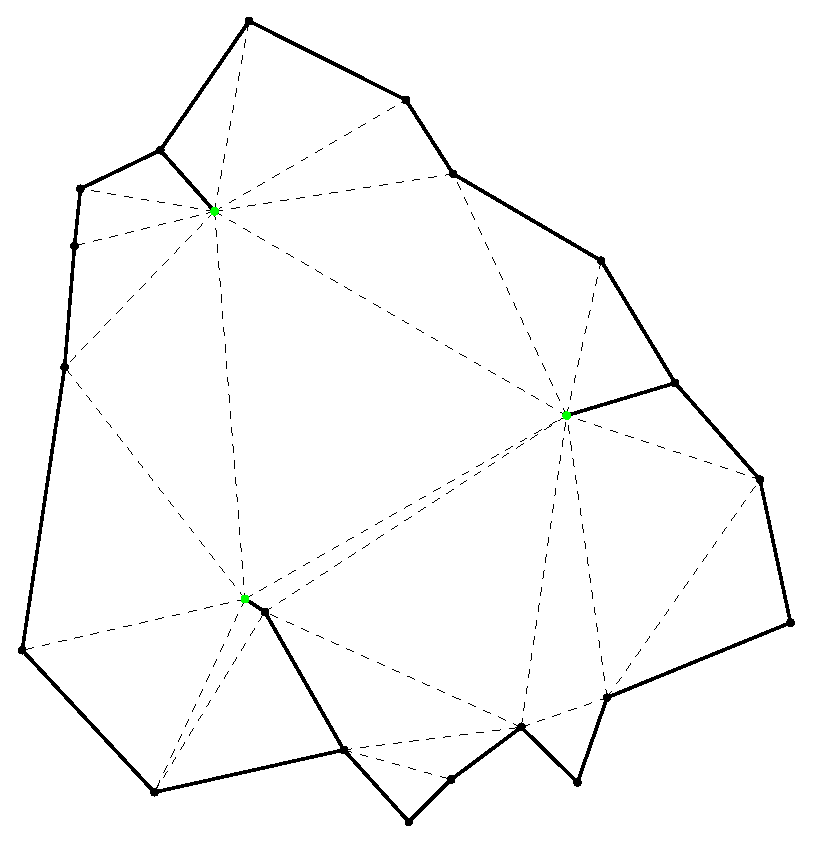
\includegraphics[width=0.3\textwidth, ]{be3split1}}\hspace{0.5cm}
\subfigure[]{\label{fig:besplited}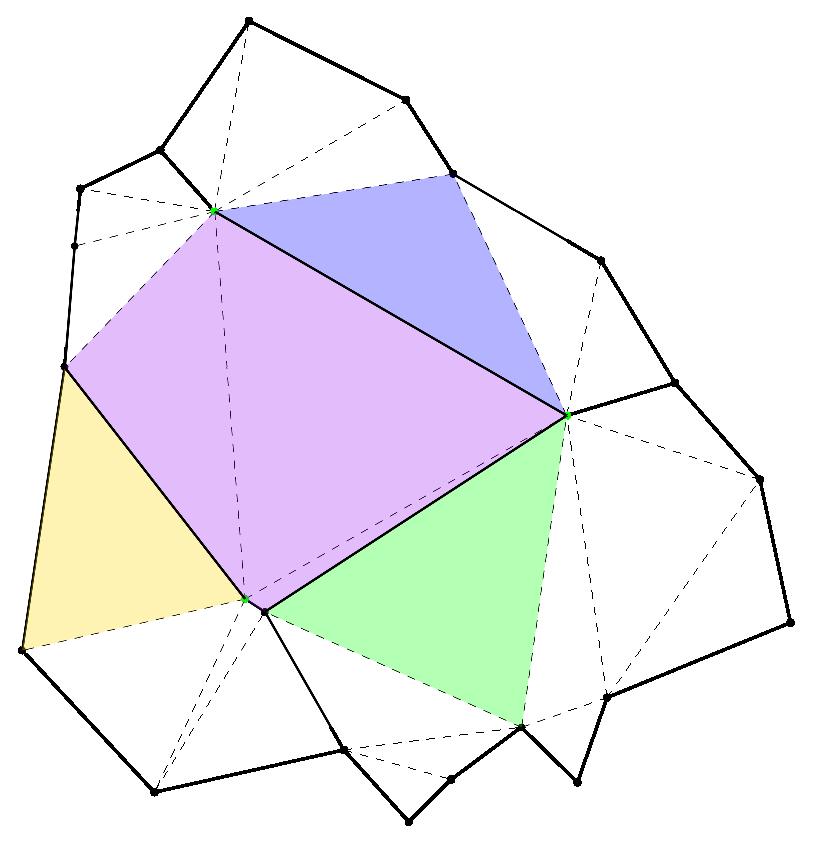
\includegraphics[width=0.3\textwidth]{be3split2v2}}\hspace{0.5cm}
\subfigure[]{\label{fig:benewpolygons}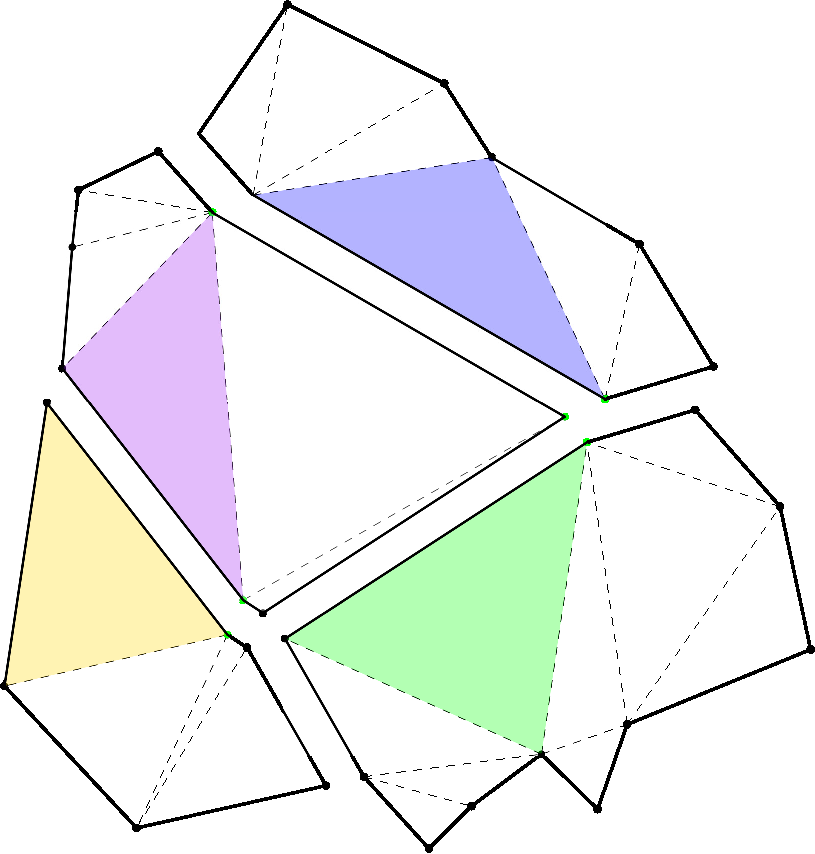
\includegraphics[width=0.3\textwidth]{be3split3v2}}
}
\caption{Example of a non-simple polygon split using barrier-edge tips. (a) Non-simple polygon. (b) Middle edges incident to barrier-edge tips labeled  as frontier-edges (solid lines) and seed triangles (colorful triangles) stored in the seed list $L_p$ and marked as 1 in the $A$ bit array. (c) The four new polygons without barrier-edge tips.  }
\label{figs:splitmid} 
\end{figure}

%\textcolor{red}{Later, the algorithm uses each triangle $t$ in the hash table $H$ to generate a new polygon (line \ref{algorepa:foreachseedtriangle}), for each $t_i \in H$ the algorithm repeats the process showed in the travel phase using $t_i$ as seed triangle to generate a new polygon $P'$, subsequently, the algorithm removes all triangles in $H$ traveled during the generation of $P'$ and store $P'$ in the mesh.}
%Note that more than one seed triangle can be stored in $H$ to build the same polygon as shown with purple triangles in  Fig. \ref{fig:besplited}. However during the polygon construction only one of them is used to build the polygon boundary and the rest is removed from $H$ while the polygon is built. Fig. \ref{fig:benewpolygons} shows the four new polygons after the split and the seed triangles used to generate them.



%but each triangle $t'$ reached during the travel is verified if $t'$ is in $H$. If it is the case, then the $'t$ is removed from $H$ to avoid generate the same polygon several times. \textcolor{blue}{This can be seen in Fig. \ref{fig:besplited}, there are three purple triangles, but just one is chosen from $H$ to generate the new polygon, during its generation two purple triangles are removed from $H$ to avoid generate the same polygon again. Fig. \ref{fig:besplited} shows the new polygon after the split and the seed triangles that generate them.}  %Fig. \ref{fig:benewpolygons} shows the final result of use the travel phase with red triangles in  Fig. \ref{fig:besplited}. 

%Later, the algorithm uses each triangle $t$ in the hash table $H$ to generate a new polygon (line \ref{algorepa:foreachseedtriangle}), for each $t \in H$ the algorithm repeats the travel phase, but each triangle $t'$ reached during the travel is verified if $t'$ is in $H$. If it is the case, then the $'t$ is removed from $H$ to avoid generate the same polygon several times. \textcolor{blue}{This can be seen in Fig. \ref{fig:besplited}, there are three purple triangles, but just one is chosen from $H$ to generate the new polygon, during its generation two purple triangles are removed from $H$ to avoid generate the same polygon again. Fig. \ref{fig:besplited} shows the new polygon after the split and the seed triangles that generate them.}  %Fig. \ref{fig:benewpolygons} shows the final result of use the travel phase with red triangles in  Fig. \ref{fig:besplited}. 







% the algorithm takes care of selecting the best according to some quality criteria. 

%For each polygon $P$, the algorithm starts counting the number $\#b$ of barrier-edge tips. This is done by compare pair of continuous edges of the polygon and see if they are equal. If there isn't barrier-edge tips the polygon is saved as part of the mesh. Otherwise, the polygon is split to remove all the barrier-edges. 

%To repair non-simple polygons, the algorithm uses the barrier-edges and internal-edges of the triangulation to split them into simple ones. So, we avoid to check intersections between inserted edges and the polygon boundary.
%To split the polygon,  %the algorithm search by all the barrier-edge tips and label the middle edge of each one as a frontier-edge and save

%\textcolor{blue}{The algorithm uses the barrier-edges and internal-edges of the triangulation to split them into simple ones. So, we avoid to check intersections between inserted edges and the polygon boundary}. The process of splitting is the following: For each barrier-edge tip $b_i$ in a polygon $P$, the algorithm count the number $deg(b_i)$ of incident internal-edges to $b_i$ in the original triangulation, if $deg(b_i)$ is odd the algorithm label the middle edge as frontier-edge, else, the algorithm choose any of middle edges to label as frontier-edge. In both cases, two triangles adjacent to the edge are saved in a hash table $H$ to use one of them a seed.

%After, the algorithm uses the triangles in $H$ to generate new polygons without barrier-edge tips. For each triangle $t_i \in H$ is used the function showed in \S\ref{subsec:Travelpohase}, but for each new triangle $t'$ reached is verified if $t'$ is in $H$, in that case $t'$ is removed from $H$ to avoid use $t'$ as seed an repeat the same polygon.




%After, a iteration is made over all elements in the hash table $H$. 
% This process is shown in Fig. \ref{figs:splitmid}.

%The process of split is the follow: For each barrier-edge tip $b_i$ in a polygon $P$, the algorithm count the number $deg(b_i)$ of adjacent internal-edges to $b_i$ in the original triangulation, if $deg(b_i)$ is odd the algorithm choose the middle edge to split the polygon, else, the algorithm choose any of middle edges to split the polygon. This process is shown in Fig. \ref{figs:splitmid}.  



% - Se inicializa la tabla de hash
%- Se recorre todo el polytope buscando BET}
%- Cuando se encuentra uno, se busca la arista de almedio, se marca como un frontier-edge y se guardan sus dos triangulos adjyancetes en una tabla hash
% - Se usan los triangulos de la tabla de hash para generar los nuevos pligonos
% - Mientras se viaja a por el poligono, se verifica si este está en la tabla de hash, si lo está se elimina
% - Proceso se repite hasta que no hayan más triangulos en la tabla de hash.


%When a polygon $P$ is generated the algorithm count the number $\#b$ of barrier-edge tips, this is done by compare pair of continuous edges of the polygon and see if they are equal. If there isn't barrier-edge tips the polygon is saved as part of the mesh, else, the polygon is call to split in two recursively until remove all the barrier-edges. 

%The process of split is the follow: Be $b_i$ a barrier-edge tip in a polygon $P$, the algorithm count the number $deg(b_i)$ of adjacent edges to $b_i$ in the original triangulation, if $deg(b_i)$ is odd the algorithm choose the middle edge to split the polygon, else, the algorithm choose any of middle edges to split the polygon. This process is shown in Fig. \ref{figs:splitmid}.



%The number of polygon generates after the split is at the most $(\#b + 1)$. The reason that this process is recursive is due to special cases where the edge choose to split $P$ contains two barrier-edge, so $#b$ needs to be calculate after each split.

\subsection{Computational Complexity Analysis}
\label{sub:Complexity Analysis}

In this section, we analyze the computational complexity of  the whole algorithm. Let  $n$ be the initial number of points, $m$ the number of triangles of the input triangulation, $m_i$ the number of triangles of the terminal-edge region $R_i$ used to generate the simple or non-simple  polygon $P_i$% and $b_i$ the number of barrier-edge tips of $P_i$.  

\begin{enumerate}
    % \item[0.] \textbf{Initial Triangulation:} The cost of generate a Delaunay Triangulation from a random set of points is $O(n\, log\, n)$.
    \item \textbf{Label Phase.} This phase uses three iterations of cost $O(m)$, one to label longest-edges, one to identify  terminal-edges and another to store seed triangles.
    \item \textbf{Traversal Phase.} This phase calls Algorithm \ref{algo:travelphase} to build one polygon simple or not simple. The construction of polygon $P_i$ has cost $O(m_i)$. Each triangle is visited  three times by Lemma \ref{l:lemmatravelphase} in the worst case (when a triangle does not have frontier-edges). As each terminal-edge region covers the whole domain without overlapping, then this phase  costs $O(m)$.
    % The complexity of this depends on the hash table and the polygon generation.
    %\item \textbf{Non-simple polygon reparation phase:} For each barrier-edge tip $b_j$ in  polygon $P_i$, the computation of $deg(b_j)$ visit the triangles that are incident to  $b_j$. Since $m_i$ is the number of triangles of $P_i$,  the labeling of internal-edges as frontier-edges  is  cost is $O(m_i)$.  The maximum number of triangles stored in the hash table is $2*b_i < k$, so building the hash table has a cost of $O(m_i)$. Using an open hash, each search and deletion has a cost of $O(1)$. The cost of building the $O(\#b)$  new polygons cost $O(k)$, since new polygons uses the same $k$ numbers of  triangles to be built, each triangle is just visited at least 3 times in the worst case. If all the polygons generated in travel phase have barrier-edge tips, this process has a final cost of $O(n)$.
    %\item {\bf Non-simple polygon reparation phase}. This phase calls algorithm~\ref{algo:reparationphase} to divide one non-simple polygon $P_i$ into simple ones. The cost depends on the number of visited triangles and this value depends on the number of barrier-edge tips $#b_i$ and the degree of each one. The labeling of internal edges as frontier edges visits a number of triangles defined by $M_i =$ $\sum_{j=1}^{\#b_i}deg(b_i^j)$, where $M_i \leq #b_i*m_i$. 
    %SE  PUEDE ACOTAR  POR ORDEN por $m_i$. Building  the new polygons is $O(m_i)$ because they do not overlap. Experimentally we have observed that the number of non-simple polygons is very low with respect to the total number of polygons. But  in case all polygons built from terminal-edge regions are non-simple,  the total cost would be $O(m)$. 
    
    \item {\bf Non-simple Polygon Reparation phase}. This phase calls Algorithm~\ref{algo:reparationphase} to divide one non-simple polygon $P_i$ into simple ones. 
    % This process only occurs in non-simple polygons. The first part of the algorithm, label internal-edge has cost equal to the cost calculate $deg(b_i)$, the number of internal-edges of each barrier-edge tip $b_i$ in $P_i$. This cost can be defined as
    % $ M_i = \sum_{b_i \in P_i}^{   } deg(b_i)
    %  M_i = \sum_{j=1}^{\#b}deg(b_{j}^i) \leq avg\{deg(b_i)\}*\#b \mbox{ with }M_i \approx m_i$
    By Lemma \ref{lemma:degReparation},  each triangle $t \in R_i$ is visited at most $3$ times, so the computation of  $deg(b)$, $\forall b \in R_i$ is  $O(m_i)$. The partition of $P_i$ into simple polygons has then a cost $O(m_i)$ because the new simple polygons  do not overlap and the algorithm only travels inside their triangles. Finally, the cost to repair all non-simple polygons is bounded $O(m)$.
    %of this phase is $O(m_i)$. As this phase only happens when there are regions with barrier-edge tips, then the final cost is equal to the sum of all of them $O(B)$, with $B$ the number of regions with barrier-edge tips in the mesh.
    
    
    %\textcolor{red}{Note if the initial triangulation is a Delaunay triangulation, the number of $deg(b_j^i)$ is expected to be $6$ in average. So $M_i$ can be narrow down by $O(\#b^i)$, as $\#b^i < m_i$, the cost of labeling middle internal-edge has cost $O(m_i)$. Building all new polygons has cost $O(m_i)$ because they do not overlap and the algorithm only travels inside the triangles of them. Finally, the cost of this phase is $O(m_i)$.}
    
    
    %Experimentally we have observed that the number of non-simple polygons is very low with respect to the total number of polygons. But  in case all polygons built from terminal-edge regions are non-simple,  the total cost would be $O(m)$. 
\end{enumerate}

\noindent
%As result, the whole algorithm has a cost $O(m)$, or $O(n)$ because it is known that $m=O(n)$. If the cost of the initial triangulation is added,  $O(n\,log\,n)$ should be added in case of using Delaunay triangulations.
\noindent
As result, the computational complexity of the whole algorithm is  $O(n)$ ($m = O(n)$).
With respect to the memory usage, the cost is $O(n)$ too. The Vertex array has size $2n$, the Triangle and Neighbor arrays have size $3n$. The number of final polygons in the mesh is less than the number of triangles in the input triangulation, i.e., bounded by $m$.


\subsection{Impact of the initial triangulation}

As mentioned above, the polygons inside a Polylla mesh depend on the initial triangulation. Any triangulation can be used as input.  Fig~\ref{figs:diff_triangulation} shows three different triangulations for the same point distribution generated using  algorithms available in the {\em 2D  Triangulations} package of the CGAL library~\cite{cgal:y-t2-21b}. Fig.~\ref{fig:DIFFrandomPolylla} is a Polylla mesh built from the triangulation generated by the incremental algorithm 
%provided by CGAL\cite{cgal:y-t2-21b} 
without  edge-flips (Fig~\ref{fig:DIFFrandomTriangulation}). The Polylla mesh in Fig~\ref{fig:DIFFregularPolylla} was built from a regular triangulation~\cite{BOISSONNAT20025} (a weighted triangulation) with random weights shown in Fig~\ref{fig:DIFFregularTriangulation}, and Fig.~\ref{fig:DIFFdelaunayPolylla} shows a Polylla mesh generated from the Delaunay triangulation drawn in Fig~\ref{fig:DIFFrandomdelaunay}. As expected, the shape of the resulting polygons is notoriously different. In order to see the differences, Table \ref{table:qualitycomp} shows for each mesh, the minimum and maximum interior angle of both the input triangulation and the generated polygon meshes, the number of polygons and the average number of edges per polygon. It can be observed that polygon meshes have a minimum interior angle greater than the minimum angle of the corresponding triangulation. Since the Polylla algorithm joins triangles to generate  polygons, the lower bound for the minimum interior angle of any polygon is the minimum angle of the input triangulation. In the case of maximum angles, the maximum angle of a Polylla mesh is usually larger than the maximum angle of the input triangulation because a Polylla's polygons can be nonconvex polygons. It seems that  Polylla meshes generated from  Delaunay triangulations tends to contain less polygons and  polygons defined with more edges than the ones obtained from other triangulations. Further research is necessary to probe these findings.

\begin{figure}[!h]
\centering     %%% not \center
\subfigure[%random triangulation
]{\label{fig:DIFFrandomTriangulation}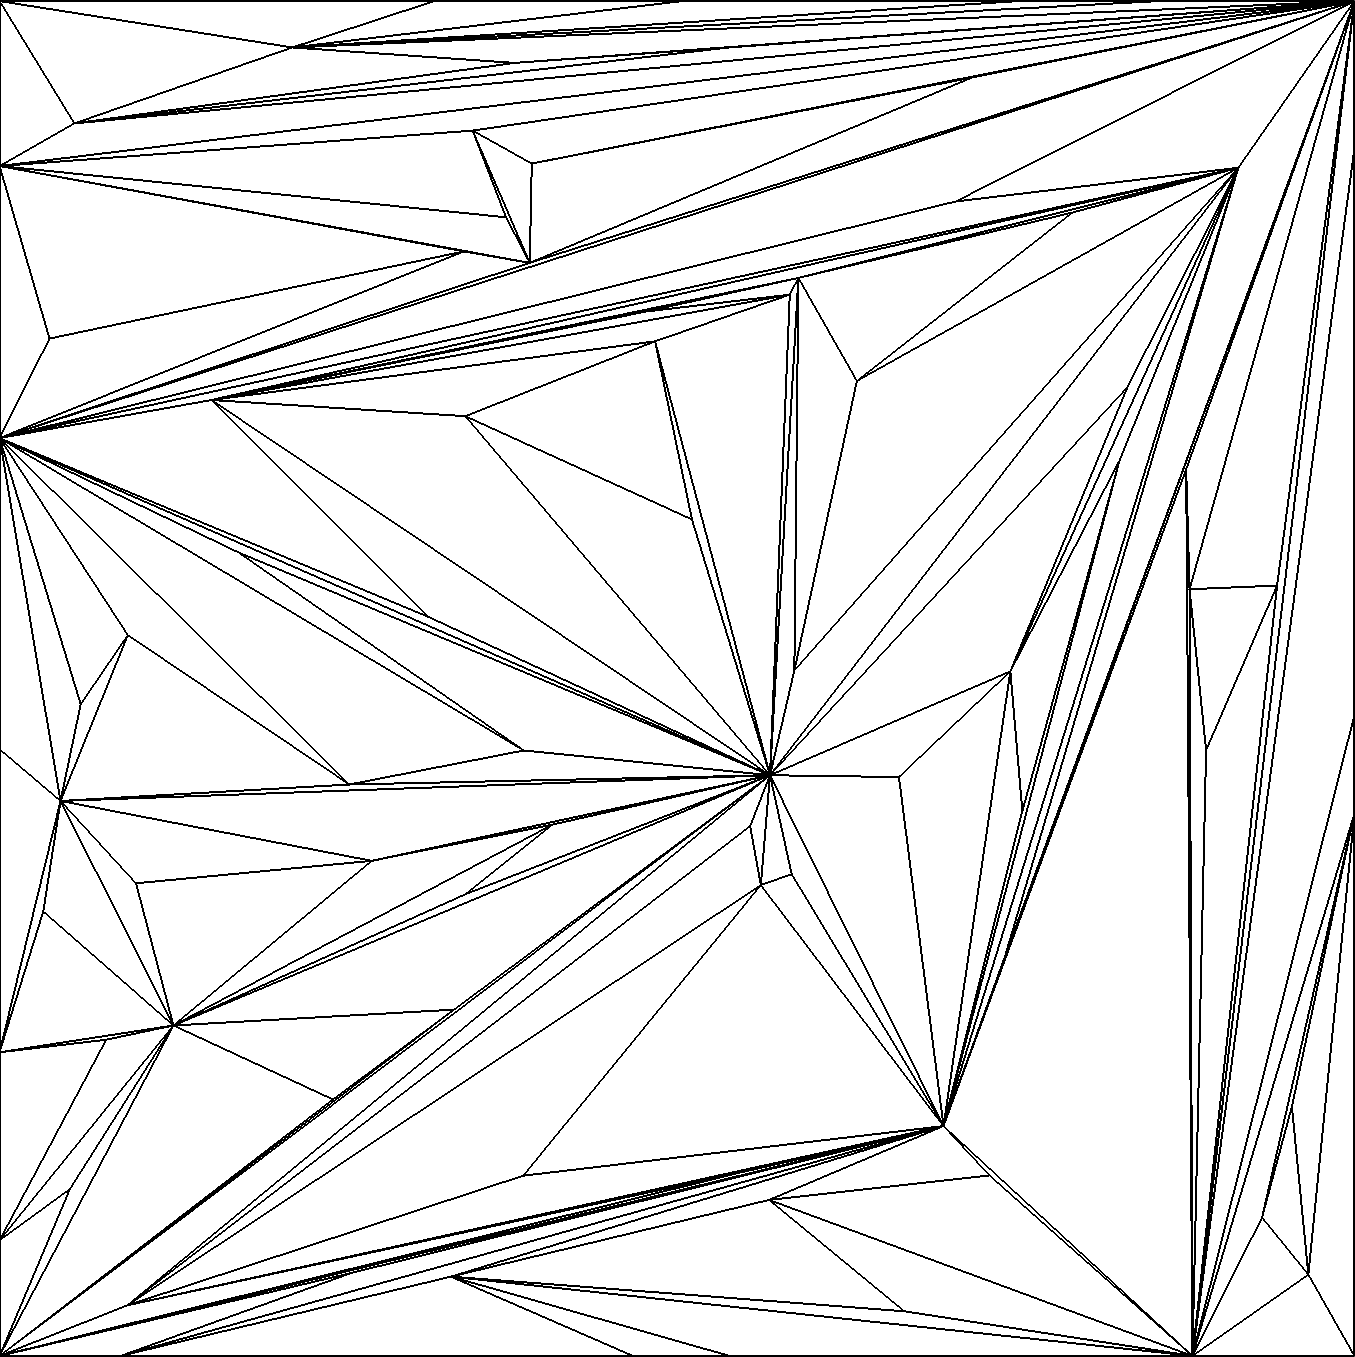
\includegraphics[width=0.25\textwidth]{TRrandom.png}} 
\subfigure[%random triangulation
]{\label{fig:DIFFregularTriangulation}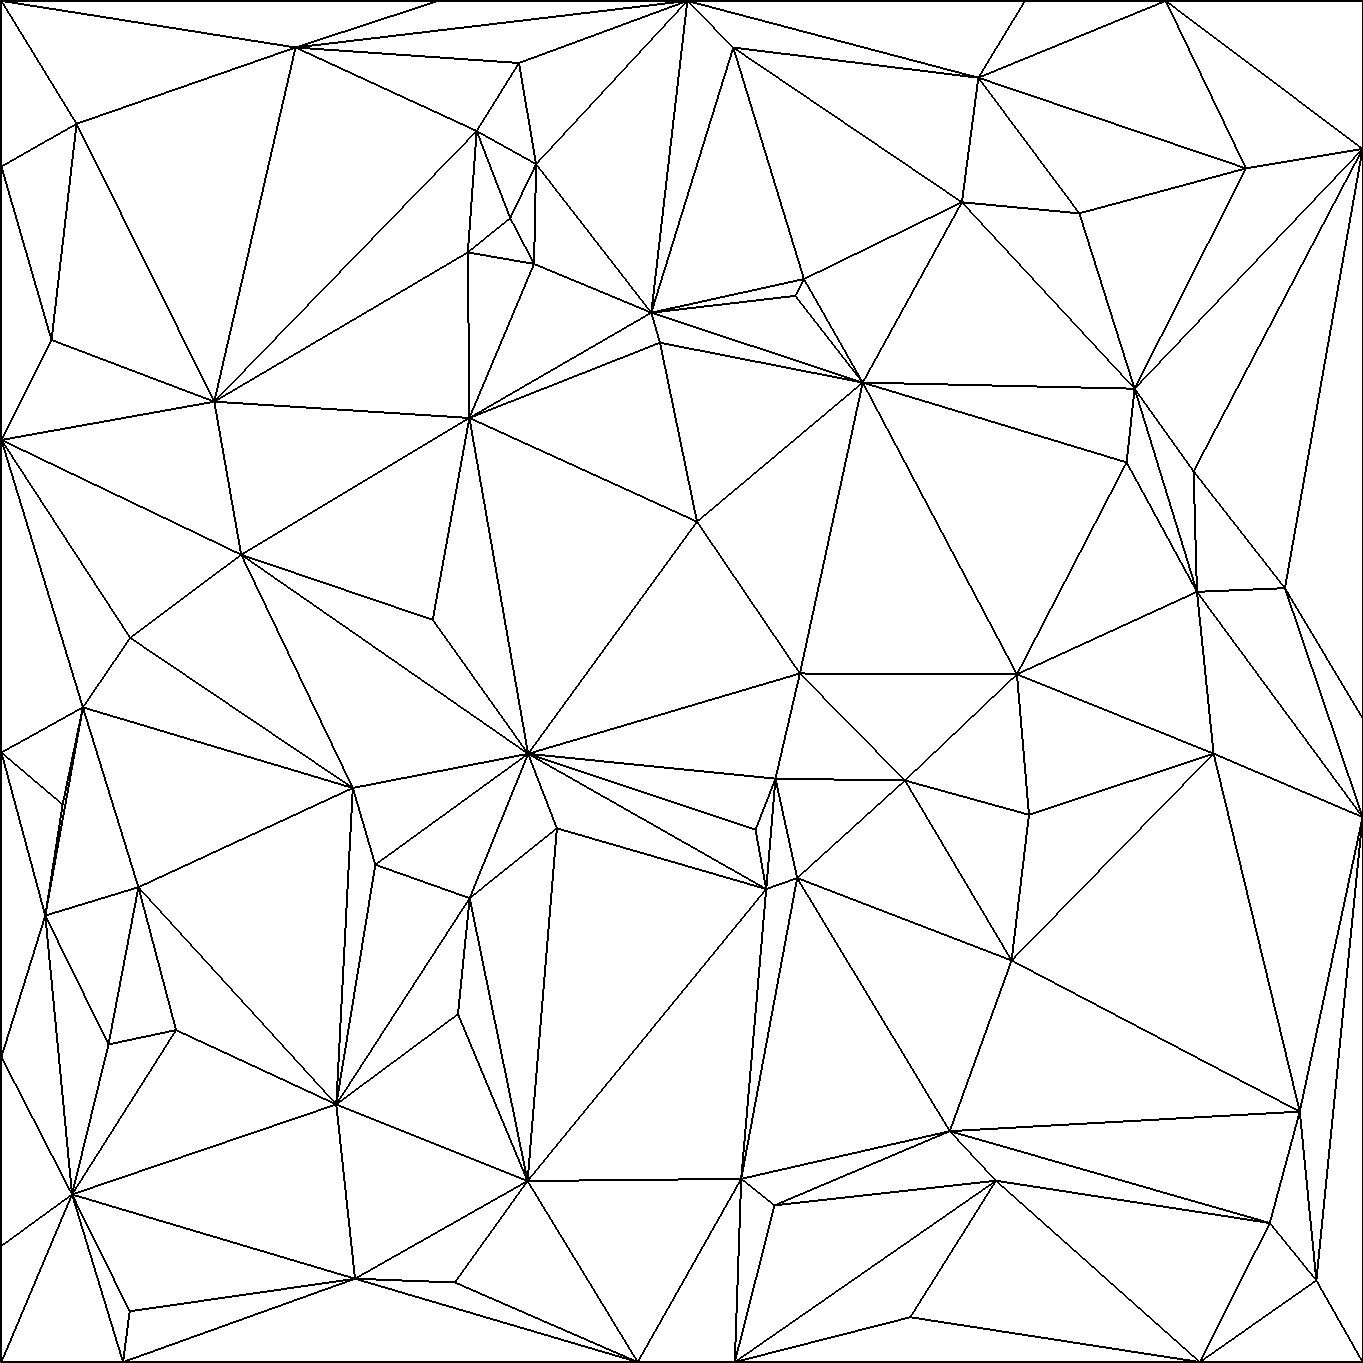
\includegraphics[width=0.25\textwidth]{TRregular.png}} 
\subfigure[%Delaunay triangulation
]{\label{fig:DIFFrandomdelaunay}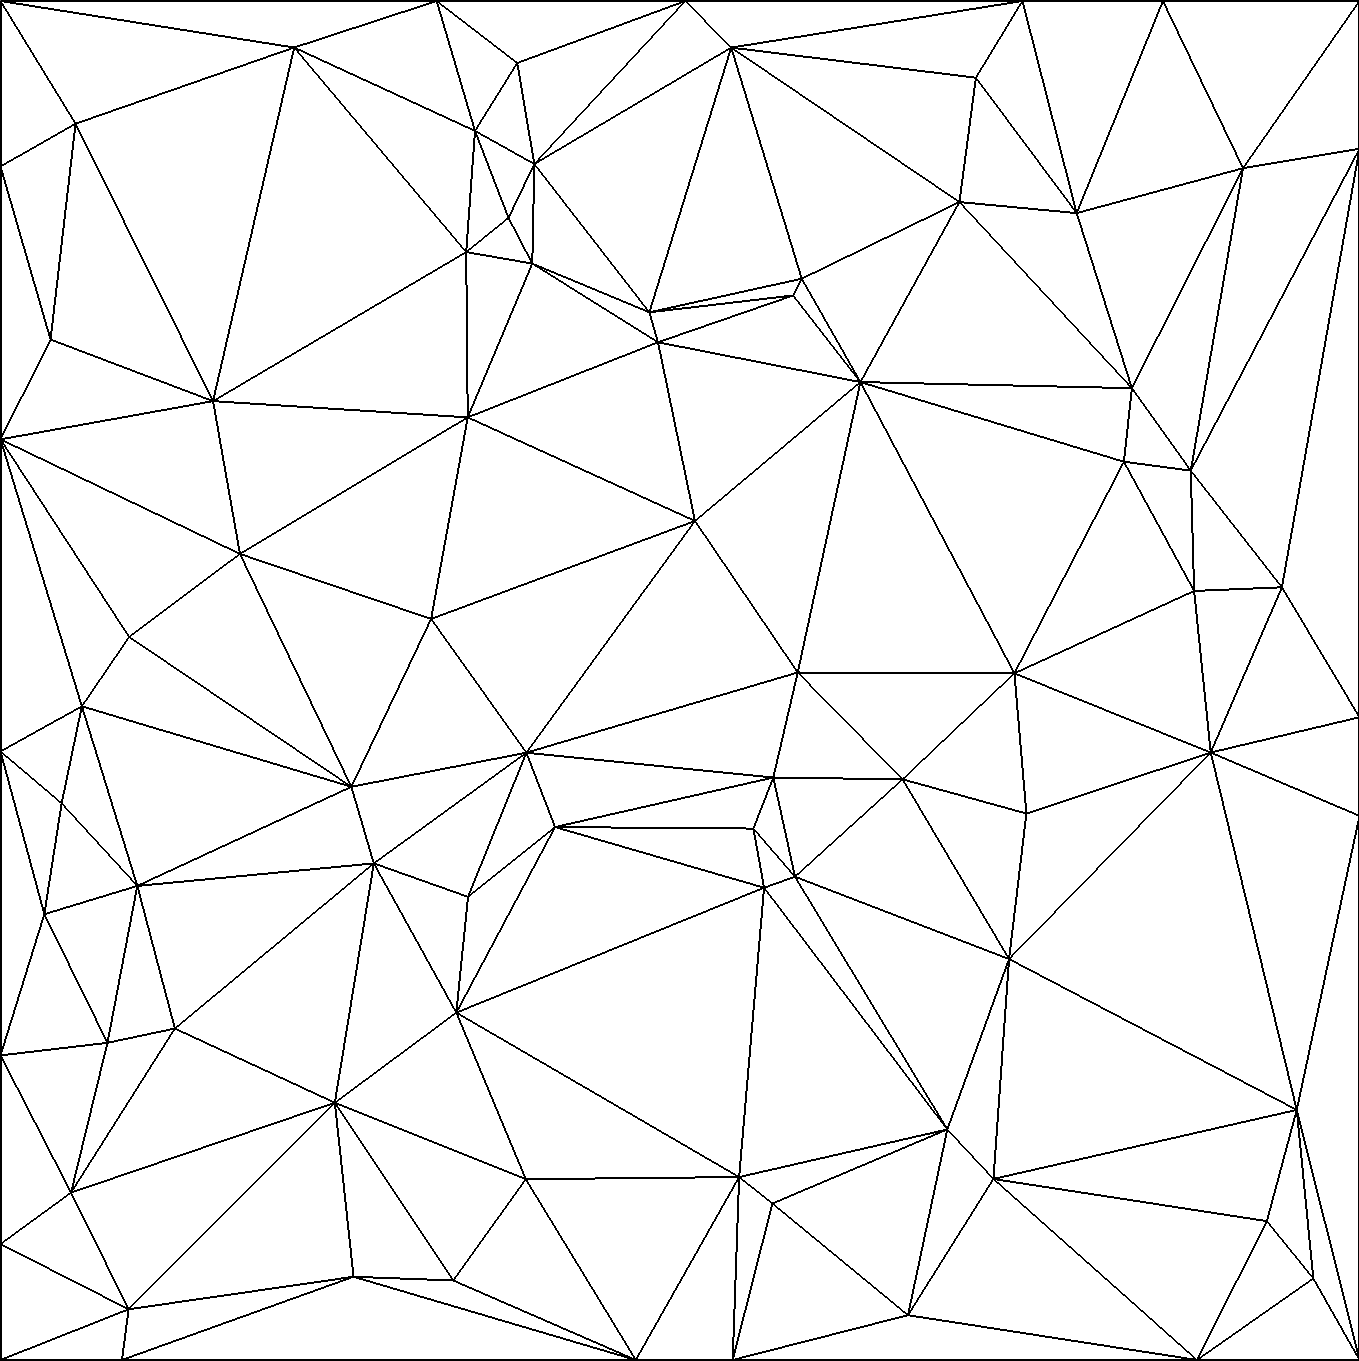
\includegraphics[width=0.25\textwidth]{TRdelaunay.png}} 
\subfigure[%random triangulation
]{\label{fig:DIFFrandomPolylla}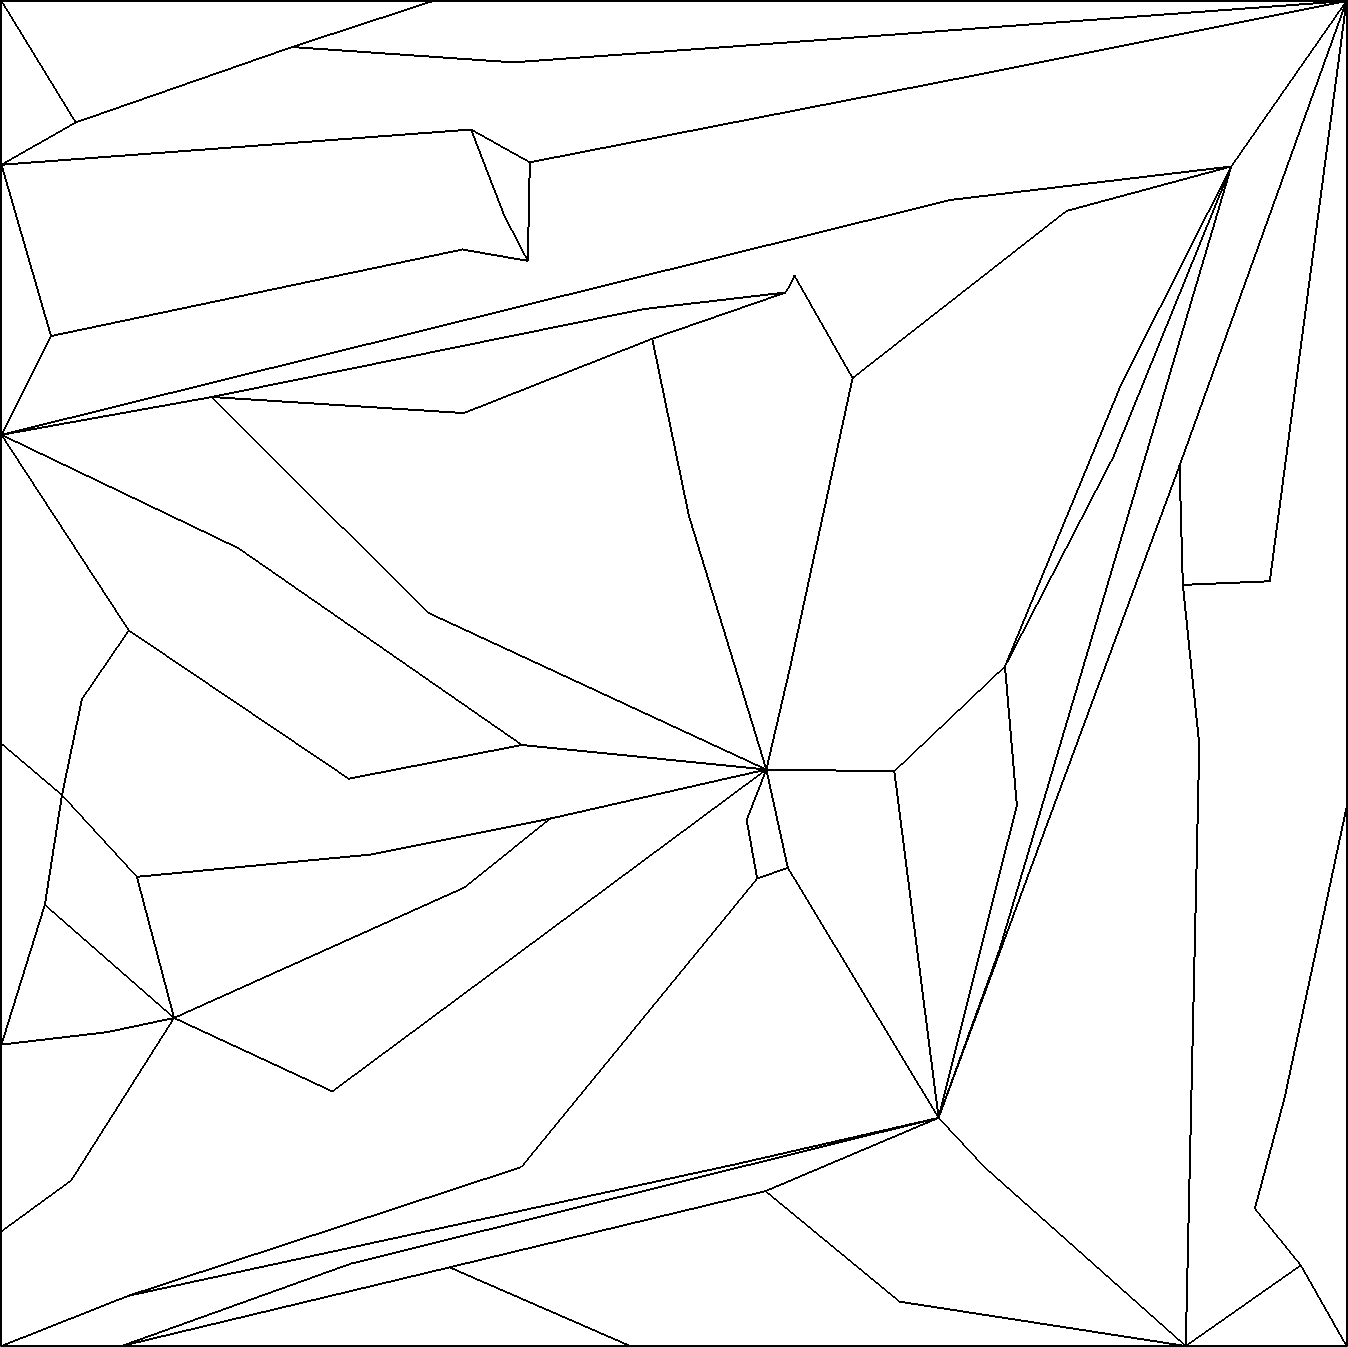
\includegraphics[width=0.25\textwidth]{polyllarandom.png}} 
\subfigure[%random triangulation
]{\label{fig:DIFFregularPolylla}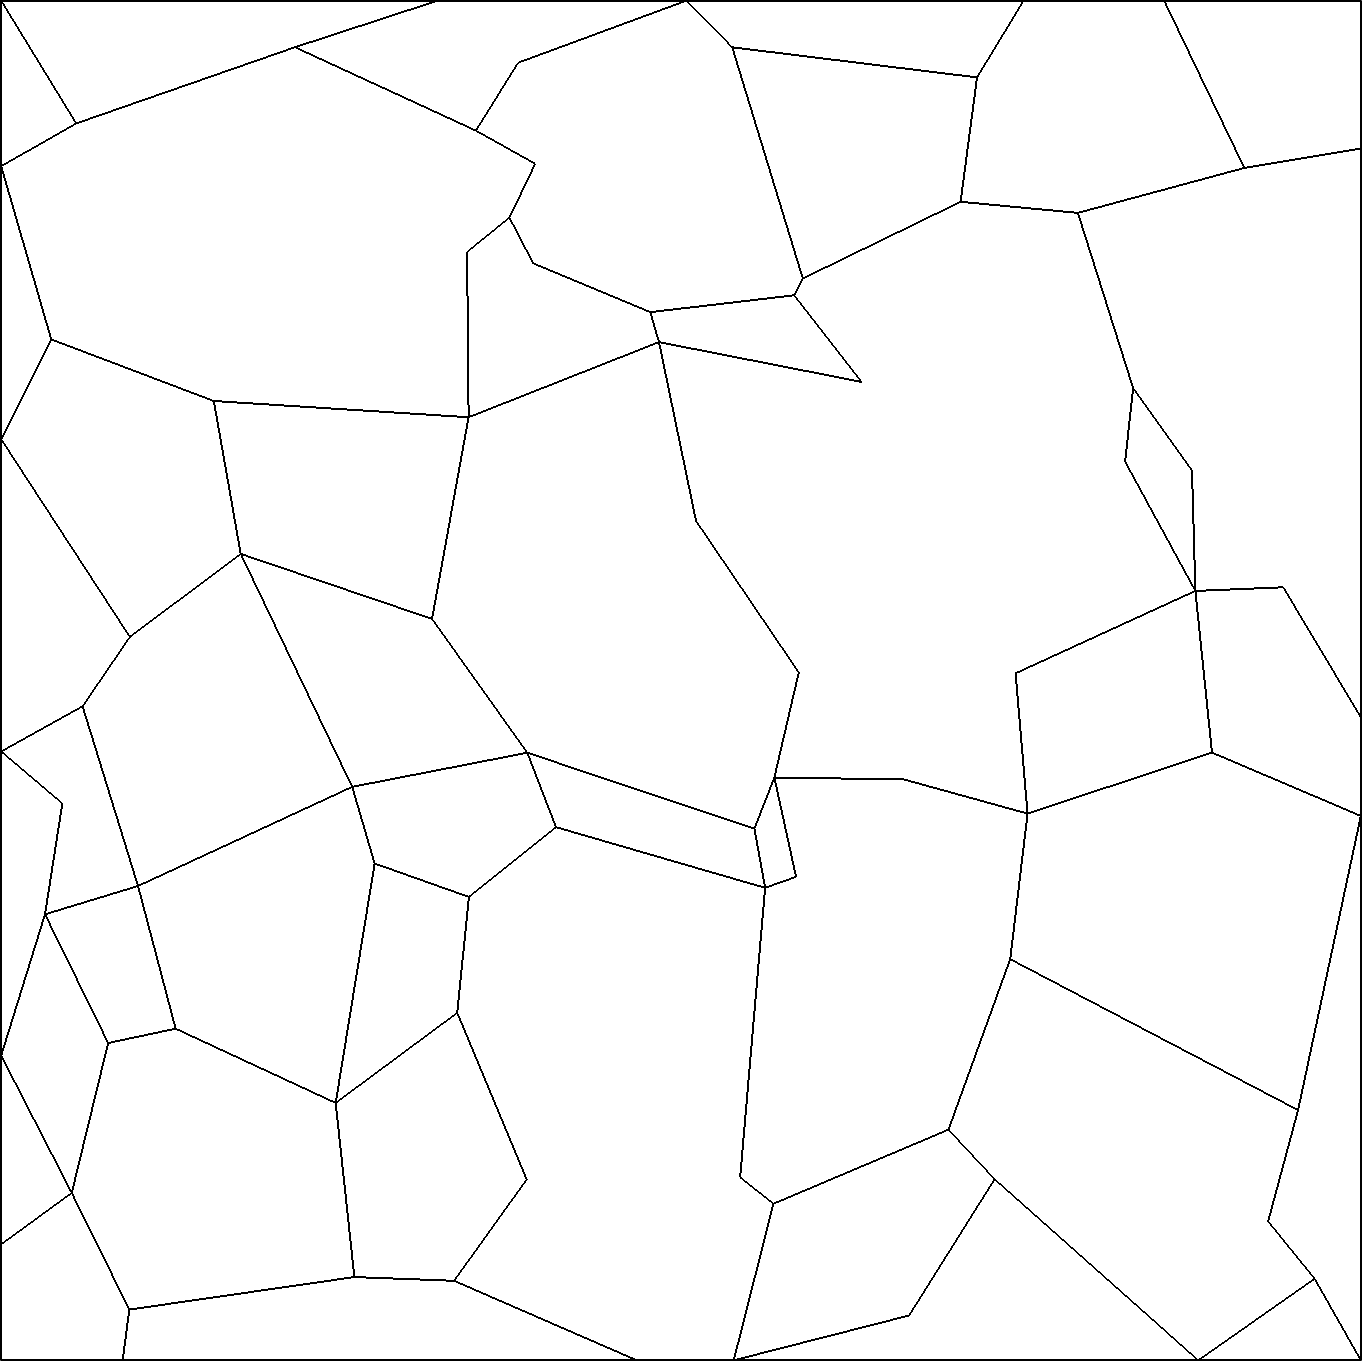
\includegraphics[width=0.25\textwidth]{polyllaregular.png}} 
\subfigure[%Delaunay triangulation
]{\label{fig:DIFFdelaunayPolylla}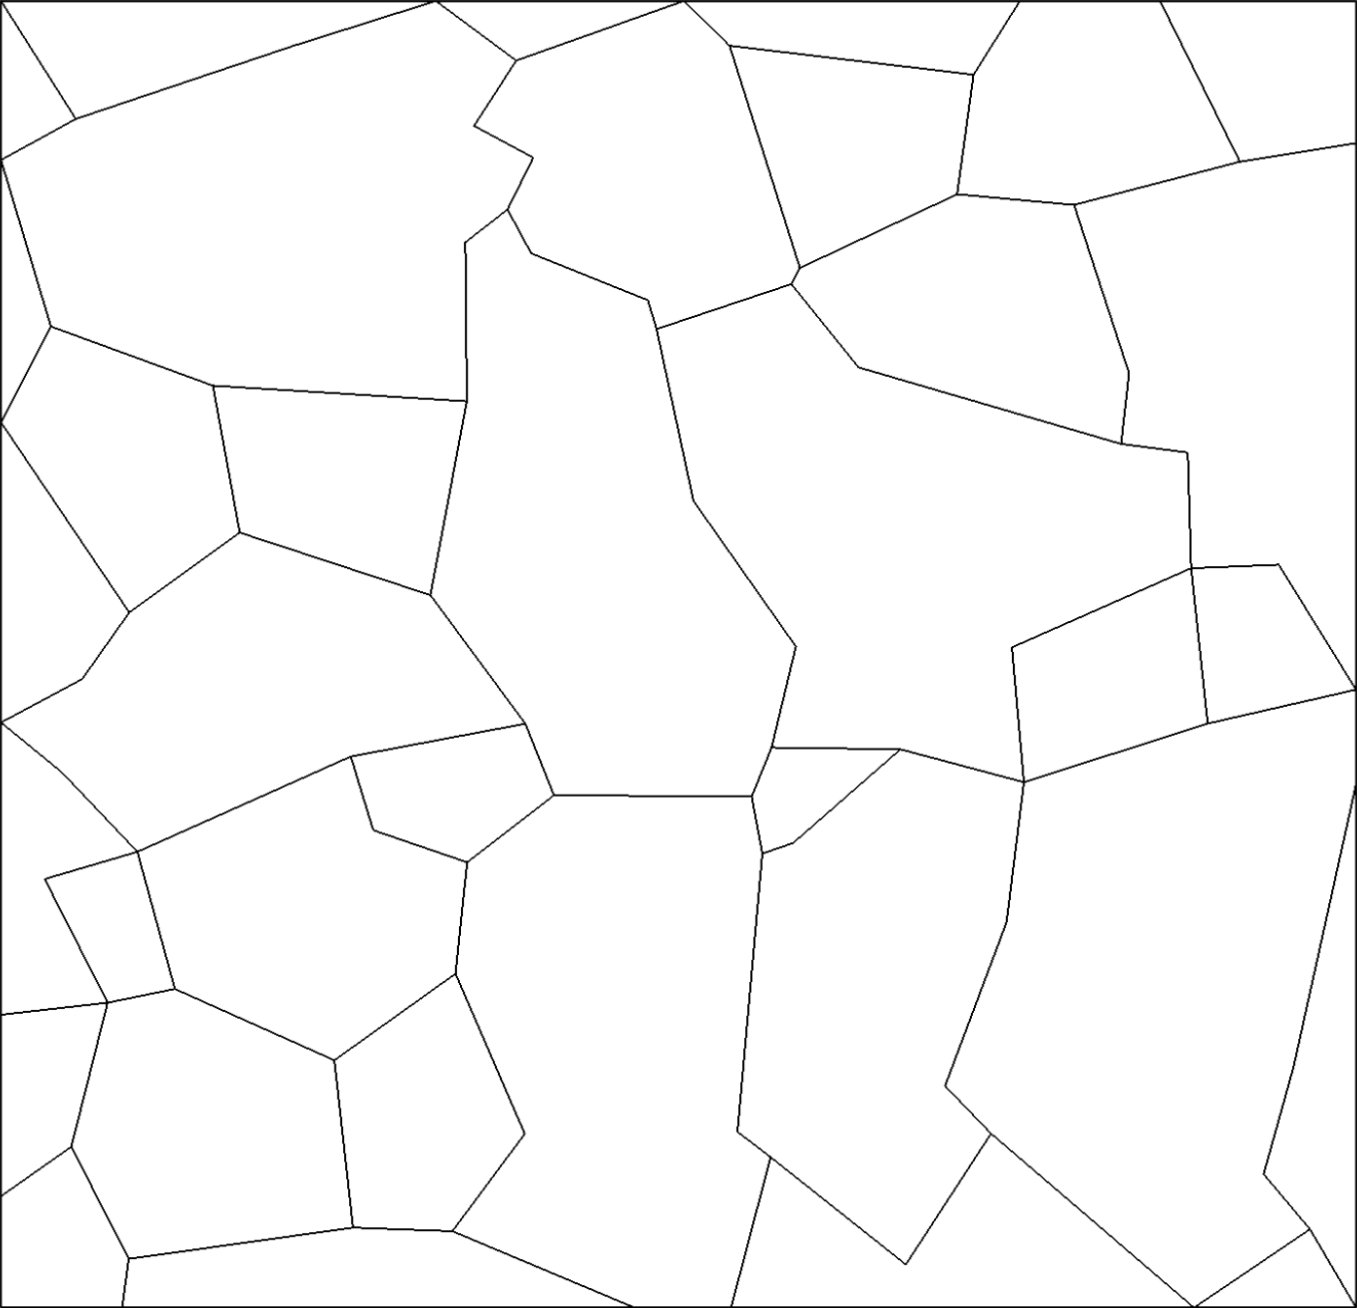
\includegraphics[width=0.26\textwidth]{polylladelaunay.png}} 
%\subfigure[]{\label{fig:DIFFEquirateral}\includesvg[width=0.4\textwidth]{autodata.svg}}
    \caption{Polylla meshes generated from different kind of initial triangulations over the same input points. Triangulations were generated using the {\em 2D  Triangulations}  package of CGAL library~\cite{cgal:y-t2-21b}. (a) Triangulation generated by the incremental algorithm, (b) regular triangulation generated using random weights, (c) Delaunay triangulation, (d) Polylla mesh generated from the triangulation (a), (e) Polylla mesh generated from the triangulation (b), and (f) Polylla mesh generated from the triangulation (c).}

\label{figs:diff_triangulation} 
\end{figure}





\begin{table}[!h]
\centering
\begin{tabular}{l|rr|rrrr|}
\cmidrule{2-7} \addlinespace[-.6em]
& \multicolumn{2}{c|}{\begin{tabular}[c]{@{}c@{}}Delaunay\\ Triangulation\end{tabular}} & \multicolumn{4}{c|}{Polylla Mesh}\\ \vspace{-1.5em}\\  \cmidrule{2-7}\addlinespace[-0.6em] & \multicolumn{1}{c|}{\begin{tabular}[c]{@{}c@{}}Min\\ Angle\end{tabular}} & \multicolumn{1}{c|}{\begin{tabular}[c]{@{}c@{}}Max\\ Angle\end{tabular}} & \multicolumn{1}{c|}{\begin{tabular}[c]{@{}c@{}}Polylla's\\ Polygons\end{tabular}} & \multicolumn{1}{c|}{\begin{tabular}[c]{@{}c@{}}Min\\ Angle\end{tabular}} & \multicolumn{1}{c|}{\begin{tabular}[c]{@{}c@{}}Max\\ Angle\end{tabular}} & \multicolumn{1}{c|}{\begin{tabular}[c]{@{}c@{}}Edges per\\  Polygon\end{tabular}} \\ \hline
\multicolumn{1}{|l|}{\begin{tabular}[c]{@{}l@{}}Incremental\\ Triangulation\end{tabular}} & \multicolumn{1}{r|}{0.027}                                               & 179.87                                                                   & \multicolumn{1}{r|}{41}                                                           & \multicolumn{1}{r|}{0.36}                                                & \multicolumn{1}{r|}{303.16}                                              & 5.65                                                                              \\ \hline
\multicolumn{1}{|l|}{\begin{tabular}[c]{@{}l@{}}Regular\\ Triangulation\end{tabular}}     & \multicolumn{1}{r|}{1.36}                                                & 177.09                                                                   & \multicolumn{1}{r|}{45}                                                           & \multicolumn{1}{r|}{12.04}                                               & \multicolumn{1}{r|}{318.98}                                              & 5.33                                                                              \\ \hline
\multicolumn{1}{|l|}{\begin{tabular}[c]{@{}l@{}}Delaunay\\ Triangulation\end{tabular}}    & \multicolumn{1}{r|}{5.75}                                                & 158.61                                                                   & \multicolumn{1}{r|}{36}                                                           & \multicolumn{1}{r|}{12.04}                                               & \multicolumn{1}{r|}{279.22}                                              & 6.16                                                                              \\ \hline
\end{tabular}
\caption{Geometric information of  the Polylla meshes generated from different triangulations from  the same point set (150 points).}
\label{table:qualitycomp}
\end{table}



It is worth to mention that since the Polylla algorithm takes as input  a triangulation, it can process  any geometry domain that can be triangulated. This includes complex geometries with holes as  shown in Fig~\ref{figs:facePSLG}. In particular, Fig.~\ref{fig:PSLGface} shows a geometry  specified as a planar straight line graph (PLSG) obtained from~\cite{triangle2d}. Fig.~\ref{fig:PSLGface} is a Polylla mesh generated from a constrained Delaunay triangulation of \ref{fig:PSLGface26}. Fig.~\ref{fig:PSLGface220} shows a Polylla mesh from a refined  conforming Delaunay triangulation of~\ref{fig:PSLGface26}. Grey polygons are holes. The algorithm considers the edges of the holes  as border edges. Meshes generated from complex geometries representing   Chilean geographic regions can be seen in Appendix~\ref{Appendix:complexgeometries}.

\begin{figure}[!h]
\centering     %%% not \center
\subfigure[%Face PLSG from~\cite{triangle2d}
]{\label{fig:PSLGface}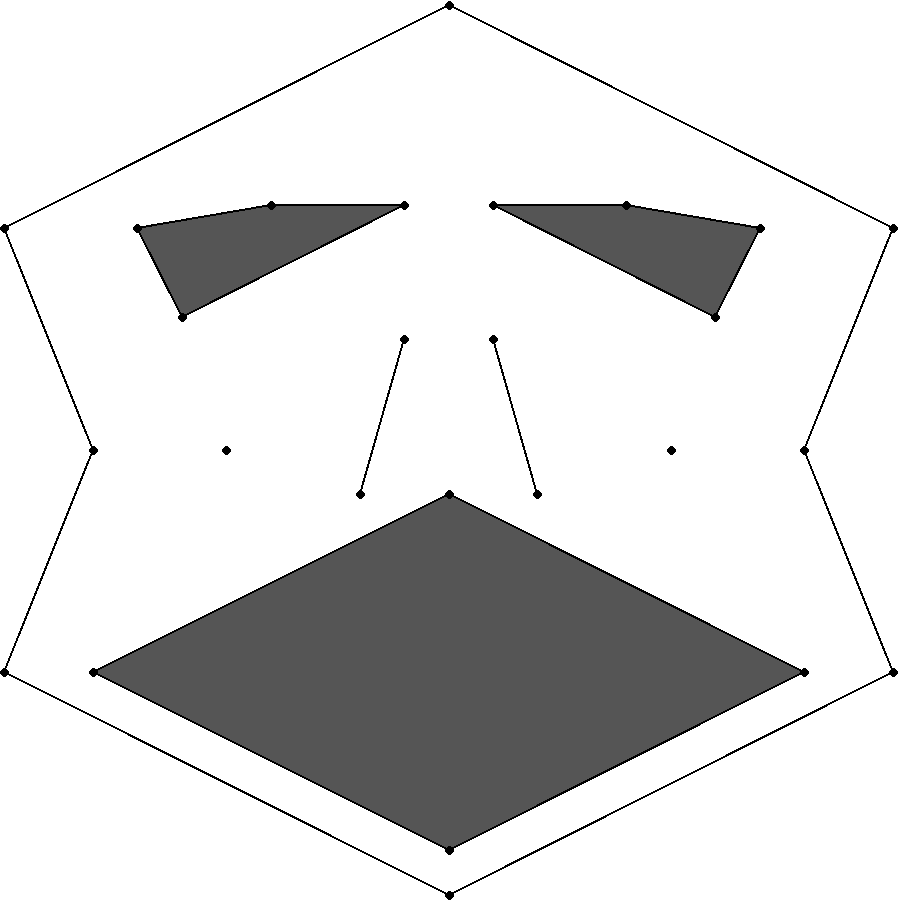
\includegraphics[width=0.3\textwidth]{faceoriginalPSLG.png}} \hspace{0.1cm}
\subfigure[%Face from Constrained Delaunay
]{\label{fig:PSLGface26}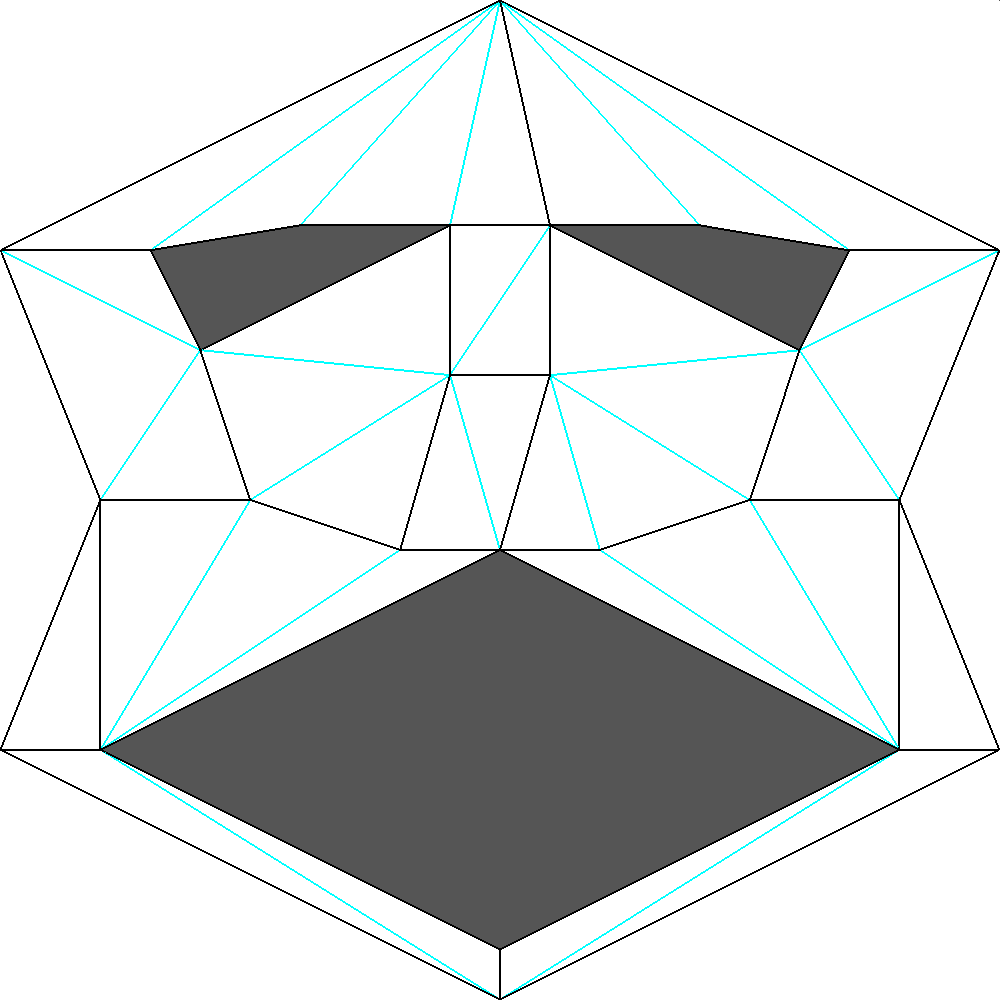
\includegraphics[width=0.3\textwidth]{facetri.png}}\hspace{0.1cm}
\subfigure[%Face from more refined triangulation
]{\label{fig:PSLGface220}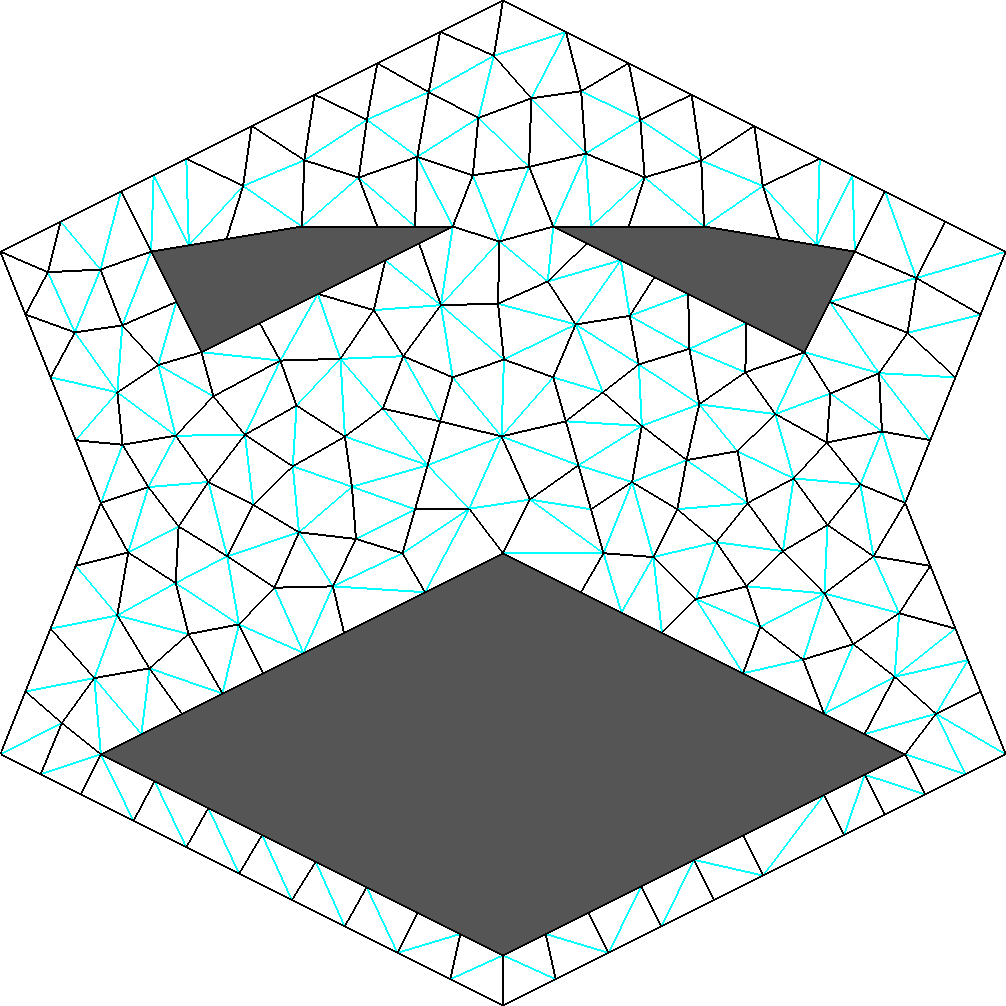
\includegraphics[width=0.3\textwidth]{facetrismall.png}}
\caption{ Polylla mesh generated from the PLSG description of the Face  taken from~\cite{triangle2d}.  The edges of the initial triangulation are drawn using black and cyan colors.
%, grey areas are holes, cyan edges are edges of the 
(b) Polygonal  mesh  obtained from the constrained Delaunay triangulation of the input geometry (26 vertices). (c) Polygonal mesh  generated from  a  refined Delaunay triangulation with 220 vertices.}
\label{figs:facePSLG} 
\end{figure}


%The polygon mesh retains the minimum angle of the input triangulation. Since  Delaunay triangulations are triangulations that maximize the minimum angle over all  triangulations for the same point set, it can be oserved that the respective polygon mesh preserves the value of this property. It seems that  Polylla meshes generated from  Delaunay triangulations tends to contain less polygons and   polygons defined with more edges than the ones obtained from other triangulations. Further research is necessary to probe these findings. %Despite the quality of both meshes, there are no significant differences between the number of polygons generated and the edges per polygons.}




% {\color{red} Theorem \ref{theorem:costPolylla} summarizes the results of this subsection.
%\begin{theorem}\label{theorem:costPolylla}
% Generation of a Polylla mesh has a cost of $O(m + B)$, with $m$ the number of triangles of the initial triangulation $\Omega$ used to generate the mesh and $B$ the number of terminal-edge regions with barrier-edge tips in $\Omega$ with a memory cost of $O(n)$. 


%With respect to the memory usage, Let be $R$ the number of terminal-edge region set without bet and $B$ the set of terminal-edge regions with bet ($B \in R$), $\sum b_i$ the sum of all barrier-edge tips in $B$. The Vertex array has size $2n$, the Triangle and Neighbor arrays have size $3n$, the seed list has size $R$ and the Mesh array has a max size of $\#R + \#B + \sum b_i$ of elements.

%With respect to the memory usage, the cost is $O(n)$. Let $n$ be the number of points of the initial triangulation. Then, the Vertex array has size $2n$, the Triangle and Neighbor arrays have size $3n$.

%let be $R$ the terminal-edge region set and $B$ the set of terminal-edge regions with barrier-edge tips ($B \in R$), $\sum b_i$ the sum of all barrier-edge tips in $B$, the seed list has size $R$ and the mesh array has a max size of $\#R + \#B + \sum b_i)$ of elements.

%The number of final polygons in the mesh is less than the number of triangles ($O(n)$) in the input triangulation. 

%\subsection{Implementation Highlights}
%\label{subsec:highlights}
%Those are highlight to considerate in our implementations.

%\begin{enumerate}
   % \item To label edges as frontier-edge the algorithm mark the adjacency as $-1$. For example, in Fig. \ref{figs:data_and_triangle}, to label red edge as frontier edge, $ADj_{3i+0}$ must change its value by $-1$. 

   % \item To improve the compute of $deg(b_i)$ we added an array that pair each vertex to one triangle adjacent to that vertex to the algorithm.

    %\item To the reparation phase a recursive function had been chosen to split polygons (split a polygon in two, and those two split them again until remove all barrier-edge tips), but to optimise the use of memory a open hash table was use. This table is an array of arbitrary length with pointers to linked list where save the seed triangles uses to generate the new polygons where each element is added to the begin of the linked list and each search operation has a delete operation inside to remove already use triangles.

%To the implementation of hash table, we use a open hash table 

%consist in two array, one contains the vertex of all polygons, and the second one and index array with the position of the last vertex of each polygon in the mesh.


%\end{enumerate}



\section{Polylla meshes vs Voronoi based meshes}
\label{sec:experimental_evaluation}

Currently, if polygonal meshes different from triangulations or quad meshes are required to solve some scientific or engineering problems,  constrained Voronoi meshes are chosen. We believe that the polygonal meshes generated by Polylla  can be an alternative to Voronoi meshes when researchers and engineers would like to model domains using arbitrary polygon shapes. That is why in this section we show standard statistics of these new polygonal meshes  in contrast to constrained  Voronoi meshes. The C++ implementation of Polylla used for the experiments can be downloaded from this repository\footnote{\url{https://github.com/ssalinasfe/Polylla-Mesh}}.

The experiment was designed as follows: the domain is a square with  a set of random points in its interior varying from $10^2$ to $10^6$. A tolerance $\pm \gamma$ is defined and used in case of  a point $p$ is too close to one square side; in that case the point $p$ is inserted in the border edge.  The statistics of the polygonal meshes generated by Polylla starting from Delaunay triangulations generated  by using Detri2 \cite{Detri2} are summarized in Table \ref{table:results}.  In the case constrained Voronoi meshes, Deldir \cite{deldir} was used to generate the meshes and to obtain their mesh  information. The statistics for the same initial points (sites) are presented in Table \ref{table:resultsVoronoi}.


%After the point sets were generated, Detri2 \cite{Detri2} was used to build the Delaunay triangulation used as initial mesh to the implementation of the algorithm. Results of the experiment are summarized in table \ref{table:results}. Deldir \cite{deldir} was used to generate the geometric information of Clipped Voronoi diagram in Table 

\begin{table}
\centering
\resizebox{\columnwidth}{!}{%
\begin{tabular}{|r|r|r|r|r|r|r|r|}
\hline
\multicolumn{1}{|c|}{\begin{tabular}[c]{@{}c@{}}Input\\ points\end{tabular}} & \multicolumn{1}{c|}{\begin{tabular}[c]{@{}c@{}}Triangles\end{tabular}} & \multicolumn{1}{c|}{\begin{tabular}[c]{@{}c@{}}Terminal-edge\\ regions\end{tabular}} & \multicolumn{1}{c|}{\begin{tabular}[c]{@{}c@{}}Polylla\\ polygons\end{tabular}} & \multicolumn{1}{c|}{\begin{tabular}[c]{@{}c@{}}Maximum barrier-edge  \\ tips in non-simple  polygons\end{tabular}} & \multicolumn{1}{c|}{\begin{tabular}[c]{@{}c@{}}Barrier-edge \\ tips\end{tabular}}  & \multicolumn{1}{c|}{\begin{tabular}[c]{@{}c@{}}Average triangles \\ per polygon\end{tabular}} & \multicolumn{1}{c|}{\begin{tabular}[c]{@{}c@{}}Average polygon\\ vertices \end{tabular}} \\ \hline
10      & 9       & 3      & 3      & 0 & 0     & 3.00 & 6.67 \\ \hline
$10^2$     & 180     & 35     & 38     & 1 & 3     & 4.74 & 6.89 \\ \hline
$10^3$    & 1911    & 281    & 305    & 2 & 24    & 6.27 & 8.30 \\ \hline
$10^4$   & 19768   & 3034   & 3228   & 4 & 194   & 6.12 & 8.13 \\ \hline
$10^5$  & 199163  & 30288  & 32271  & 4 & 1984  & 6.17 & 8.17 \\ \hline
$10^6$ & 1997497 & 302944 & 322561 & 4 & 19647 & 6.19 & 8.19 \\ \hline
\end{tabular}
}
\caption{Geometric information of Polylla mesh }%\tiny{\footnotemark barrier-edge tips}}
\label{table:results}
\end{table}

\iffalse

\begin{table}
\centering
\resizebox{\columnwidth}{!}{%
\begin{tabular}{|r|r|r|r|r|r|r|r|}
\hline
\multicolumn{1}{|c|}{\begin{tabular}[c]{@{}c@{}}Input\\ points\end{tabular}} & \multicolumn{1}{c|}{\begin{tabular}[c]{@{}c@{}}Triangle\\ number\end{tabular}} & \multicolumn{1}{c|}{\begin{tabular}[c]{@{}c@{}}Terminal-edges\\ number\end{tabular}} & \multicolumn{1}{c|}{\begin{tabular}[c]{@{}c@{}}Terminal-edge\\ polygon\end{tabular}} & \multicolumn{1}{c|}{\begin{tabular}[c]{@{}c@{}}Max bet in \\ non-simple Polygons\end{tabular}} & \multicolumn{1}{c|}{Total Bet} & \multicolumn{1}{c|}{\begin{tabular}[c]{@{}c@{}}Triangles \\ per polygon\end{tabular}} & \multicolumn{1}{c|}{\begin{tabular}[c]{@{}c@{}}Edges \\ per polygon\end{tabular}} \\ \hline
10                                                                           & 14                                                                             & 5                                                                                    & 5                                                                                    & 0                                                                                              & 0                              & 2.80                                                                                  & 5.80                                                                              \\ \hline
$10^2$                                                                       & 192                                                                            & 34                                                                                   & 38                                                                                   & 2                                                                                              & 4                              & 5.05                                                                                  & 7.18                                                                              \\ \hline
$10^3$                                                                       & 1949                                                                           & 283                                                                                  & 310                                                                                  & 2                                                                                              & 27                             & 6.29                                                                                  & 8.30                                                                              \\ \hline
$10^4$                                                                       & 19618                                                                          & 3012                                                                                 & 3192                                                                                 & 4                                                                                              & 180                            & 6.15                                                                                  & 8.15                                                                              \\ \hline
$10^5$                                                                       & 197976                                                                         & 29965                                                                                & 31902                                                                                & 4                                                                                              & 1938                           & 6.21                                                                                  & 8.21                                                                              \\ \hline
\end{tabular}
}
\caption{Geometric information of polylla mesh }%\tiny{\footnotemark barrier-edge tips}}
\label{table:results}
\end{table}
\fi


\begin{table}
\centering
\begin{tabular}{|r|r|r|r|r|}
\hline
\multicolumn{1}{|c|}{\begin{tabular}[c]{@{}c@{}}Input \\ Points\end{tabular}} & \multicolumn{1}{c|}{\begin{tabular}[c]{@{}c@{}}Voronoi \\ vertices\end{tabular}} & \multicolumn{1}{c|}{\begin{tabular}[c]{@{}c@{}}Voronoi\\ Regions\end{tabular}} & \multicolumn{1}{c|}{\begin{tabular}[c]{@{}c@{}}Voronoi\\ Edges\end{tabular}} & \multicolumn{1}{c|}{\begin{tabular}[c]{@{}c@{}}Edges\\ per Region\end{tabular}} \\ \hline
10                                                                            & 22                                                                               & 10                                                                              & 31                                                                           & 4.90                                                                             \\ \hline
$10^2$                                                                        & 202                                                                              & 100                                                                             & 301                                                                          & 5.75                                                                            \\ \hline
$10^3$                                                                        & 2002                                                                             & 1000                                                                            & 3001                                                                         & 5.90                                                                             \\ \hline
$10^4$                                                                        & 20001                                                                            & 10000                                                                           & 30001                                                                        & 5.96                                                                          \\ \hline
\end{tabular}
\caption{Geometric information of constrained Voronoi diagram }%\tiny{\footnotemark barrier-edge tips}}
\label{table:resultsVoronoi}
\end{table}

%The input geometry can be  defined by the convex hull of  random point sets or  using a  PSLG specification. The Delaunay triangulations were generated using the  Detri2 library~\cite{Detri2}.  
%Table \ref{table:results} summarizes some   statistical data of the polygonal meshes generated from random points.
In Table \ref{table:results}, we can observe that over $10^4$ input points, the number of initial triangles per polygon is $6.5$ and the number of vertices per polygon is $8.5$, both values  on average. The number of barrier-edge tips is less than $3\%$ of the number of points, so the reparation phase just adds less than $10\%$ of polygons to the mesh. If we compare Polylla meshes with the meshes generated from the Voronoi diagram, the constrained  Voronoi meshes contain 3 times more polygons than our meshes. Each Voronoi region based polygon is delimited  in average by  6 edges and  Polylla polygons by 8 edges. 
Moreover, the Polylla meshes use only the points given as input; in contrast, the Voronoi based meshes use new points, the Voronoi points, one per each triangle of the Delaunay mesh. Since the number of triangles is greater than the number of input points, the size of the Voronoi mesh is greater than the size of the Polylla  mesh not only in terms of polygons, but also in terms of mesh points.% COMO SE     VE ESTO EN LA TABLA?

It is worth mentioning that a Polylla mesh does not need to insert extra-points at the boundary to fit the domain geometry; in contrast the constrained  Voronoi mesh includes new points at the boundary/interfaces inserted while cutting the Voronoi regions that go outside the domain.  



 We have also evaluated the time performance of Polylla. The results  shown in Fig. \ref{fig:timecomp} were made on  Patagón, a computer with two Intel Xeon Platinum 8260 of 2.4Ghz, located at the  Universidad Austral de Chile \cite{patagon-uach}. The results are the average time of  five program executions with same data-set in a different core.  
 % It can be observed that the Polylla time performance scales linearly as expected. 
 The time of each phase  is included together with time to generate the initial triangulation. 
 % experiment presented in Fig. \ref{fig:timecomp} shows that the generation of a Polylla mesh is even more efficient than the generation of initial triangulation when it is a triangulation of Delaunay (and therefore, constrained Voronoi diagram). 
 Of the three phases described in section \ref{sec:the_algorithm}, the  phase that takes less time is the non-simple polygon reparation phase. The main reason is that the number of terminal-edge regions with barrier edges  is around 1\% of the total  number  terminal-edges regions formed from random point sets  as  can be seen in Fig. \ref{fig:timecomp}.
 %it is due to this phase only occurs when during the travel phase emerge polygons with barrier-edge tips, and as is presented in Fig. \ref{fig:polycomp}, the number of new polygons added due to the reparation phase, and therefore due to polygons with barrier-edge tips, is low in comparison with the number of original number of terminal-edge regions in the initial triangulation.
 The time  of the Label phase is higher than the time of the traversal phase. This can be explained due to the use of floating-point arithmetic  to calculate the length of each edge  and so to assign the proper label. 
 %to its classification, a low precision in calculation in the distance between two endpoints, of a edge, can deviates in overlapped polygons and holes in the final mesh.



%\textcolor{red}{In the comparison of time generation of Poylla meshes vs Voronoi diagram, generation of Polylla mesh is more efficient, in Fig~\ref{fig:meshesgenerator} we compared the time of the generation of Polylla meshes against the time generation of Constrained Voronoi digrams and constrained Delaunay Triangulations, implementation of constrained Delaunay triangulation was made using the package 2D triangulations of CGAL~\cite{cgal:y-t2-21b}  and the package 2D Voronoi Diagram Adaptor~\cite{cgal:k-vda2-21b} to generate the constrained Voronoi diagram, both were assessed in a CPU Intel(R) Core(TM) i5-9600K of 3.70GHz. Calculate Voronoi diagram using~\cite{cgal:k-vda2-21b} is faster than using the function dual in ~\cite{cgal:y-t2-21b}. Tested meshes were generated over a constrained L-shape domain with random points inside, this domain is used in section~\ref{sec:simulation_results} to asses Polylla meshes using the virtual element method, this domain was choose to do a fair comparison with the constrained edges of the Voronoi diagram and the constrained Delaunay triangulation, as CGAL does not have a method to add constrain edges in a Voronoi diagram, we cut each Voronoi region by calculating the intersection of each region with the L-shape domain.}

In order to compare the CPU time required to generate constrained Voronoi and Polylla meshes,  we looked for free and open source tools. The CGAL library provides  {\em  2D Voronoi Diagram Adaptor} package~\cite{cgal:k-vda2-21b} to generate Voronoi diagrams, but this package does not provide a method to cut Voronoi regions against the domain boundary. So we  implemented  a function to do this process. In contrast, Detri2~\cite{Detri2} offers a robust method to generate constrained Voronoi meshes.   Table~\ref{table:compvoropoylla} shows the cpu-times in seconds needed to generate polygonal meshes using Polylla, Detri2D and CGAL from 100000, 500000 and 1000000 points over a L-shape domain. Experiments were run in a CPU Intel(R) Core(TM) i5-9600K of 3.70GHz. Detri2d computes the CDT first and then the CVD from the CDT. That is why we included the time to generate the CDT separated from the generation of the CVD. 
The Polylla time includes only the time spent in  the three phases that processes the input triangulation to generate the polygon mesh. The CGAl algorithm to generate the VD includes generation of the Delaunay triangulation first and from this triangulation computes the Voronoi Diagram. The CVD cost in CGAL is the sum of VD and CV. This preliminary comparison shows that the time to generate a CDT using Detri2d or CGAL plus the time Polylla takes to generate the polygonal mesh is much less than the time needed for generating a CVD either using Detri2 or the CGAl library. The main reason is that constrained Voronoi based meshing algorithms require to compute and insert new points (Voronoi points), to cut Voronoi regions  and insert new boundary points. In contrast, the Polylla algorithm  just needs  to process the vertices, edges and triangles of the input triangulation.  The domain boundary is already represented by some triangle edges.

%In addition, Polylla needs as input a triangulation: so the time to generate a CDT must be added to the time associated to Polylla. 
%The Polylla time includes only the time spent in  the three phases that processes the input triangulation to generate the polygon mesh. The CGAl algorithm to generate the Voronoi diagram (VD) includes generation of the Delaunay triangulation first and from this triangulation computes the Voronoi Diagram. The cut Voronoi (CV) is the cost of intersecting each infinite Voronoi region  against the domain boundary.  The CVD cost in CGAL is the sum  of VD and CV. This preliminary comparison shows that the time to generate a CDT using Detri2d or CGAL plus the time Polylla takes to generate the polygonal mesh is much less than the time needed for generating a CVD either using Detri2 ir the CGAl library. The main reason is that constrained Voronoi based meshing algorithms require to compute and insert new points (Voronoi points), to cut Voronoi regions  and insert new boundary points. In contrast, the Polylla algorithm  just needs  to process the vertices, edges and triangles of the input triangulation.  The domain boundary is already represented by some triangle edges.


%En el caso de CGAL, CVD incluye todo el tiempo o no? Si lo incluye, creo que no deberiamos poner el CDT de CGAL. Tienes que separar el tiempo del calculo de voronoi y el recorte de las regiones.

% The generation of constrained Voronoi meshes 
% \textcolor{blue}{In the comparison of time generation of Poylla meshes vs Voronoi 
% diagram, generation of Polylla mesh is more efficient, in %Table~\ref{table:compvoropoylla} we compared the time of the generation of Polylla 
% meshes against the time generation of Constrained Voronoi digrams. 
% To the asses, we use two different Voronoi mesh generators Detri2~\cite{Detri2} and 
% CGAL~\cite{cgal:k-vda2-21b}, additionally, as Poylla meshes depend on a initial 
% triangulation, we added the cost of generate each constrained Delaunay Triangulation,
% in the case of CGAL, the times of the triangulation correspond to the package 2D %triangulations~\cite{cgal:y-t2-21b}. 

 

%Tested meshes were generated over a constrained L-shape domain with random points inside, this domain is used in section~\ref{sec:simulation_results} to asses Polylla meshes using the virtual element method, this domain was choose to do a fair comparison with the constrained edges of the Voronoi diagram and the constrained Delaunay triangulation, as CGAL does not have a method to add constrain edges in a Voronoi diagram, we cut each Voronoi region by calculating the intersection of each region with the L-shape domain. Detri2 has a robust method to generate Constrain Voronoi meshes so it did not need cut cells. Generation of Poylla meshes are clearly more efficient, it is explained due to we can work directly with vertices and edges of the initial triangulation without any addition of extra vertices, the unique geometric operation in Polylla is calculate the length of each edge of the initial triangulation, in Constrained Voronoi meshes, it is necessary to calculate each Voronoi vertex, edge and cut each Voronoi region with the constrain border.


% Please add the following required packages to your document preamble:
% \usepackage[table,xcdraw]{xcolor}
% If you use beamer only pass "xcolor=table" option, i.e. \documentclass[xcolor=table]{beamer}
%\cmidrule{3-6} \addlinespace[-.5em]
\begin{table}[]
\centering
\begin{tabular}{lr|rr|rllr|}
\cmidrule{3-8} \addlinespace[-.6em]
                               & \multicolumn{1}{c|}{}        & \multicolumn{2}{c|}{Detri2}                           & \multicolumn{4}{c|}{CGAL}                                                                                          \\ \hline
\multicolumn{1}{|l|}{Vertices} & \multicolumn{1}{c|}{Polylla} & \multicolumn{1}{c|}{CDT}   & \multicolumn{1}{c|}{CVD} & \multicolumn{1}{c|}{CDT}    & \multicolumn{1}{l|}{VD}     & \multicolumn{1}{l|}{CV}     & \multicolumn{1}{c|}{CVD} \\ \hline
\multicolumn{1}{|l|}{100000}   & 0.193                        & \multicolumn{1}{r|}{0.326} & 229.489                  & \multicolumn{1}{r|}{1.712}  & \multicolumn{1}{l|}{28.39}  & \multicolumn{1}{l|}{9.68}   & 38.07                    \\ \hline
\multicolumn{1}{|l|}{500000}   & 0.7684                       & \multicolumn{1}{r|}{1.703} & 5736.473                 & \multicolumn{1}{r|}{9.006}  & \multicolumn{1}{l|}{335.26} & \multicolumn{1}{l|}{56.16}  & 391.42                   \\ \hline
\multicolumn{1}{|l|}{1000000}  & 1.3294                       & \multicolumn{1}{r|}{3.346} & 21341.734                & \multicolumn{1}{r|}{16.082} & \multicolumn{1}{l|}{870.52} & \multicolumn{1}{l|}{120.52} & 991.04                   \\ \hline
\end{tabular}
\caption{Time comparison, in seconds, of Polylla vs Constrained Voronoi Diagram (CDV) using Detri2 and CGAL. CDT is the time to generate a Constrained Delaunay Triangulation, VD is the time of generate Voronoi Diagram, CV is the time need to cut all regions of Voronoi Diagram and CVD is the total time of generate the Constrained Voronoi Diagram. }%\tiny{\footnotemark barrier-edge tips}}
\label{table:compvoropoylla}
\end{table}



\begin{figure}
\centering     %%% not \center

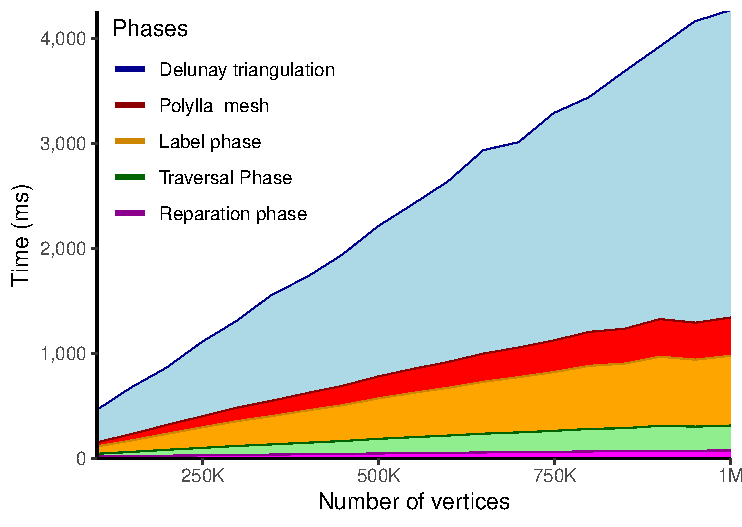
\includegraphics[width=0.5\textwidth]{timecompB}
%\includegraphics[width=0.5\textwidth]{timecompFIX}
\caption{Time performance of the  different algorithm phases. The label Polylla mesh indicates  the time of the three phases.
}
\label{fig:timecomp} 
\end{figure}


%\begin{figure}
%\centering     %%% not \center
%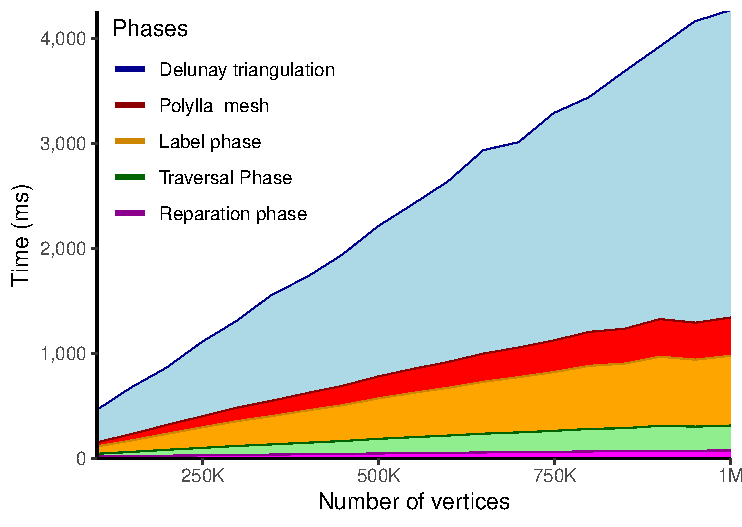
\includegraphics[width=0.5\textwidth]{timecompB}
%\includegraphics[width=0.5\textwidth]{timecompVOROPOlylla}
%\caption{\textcolor{red}{Time performance of generation of Polylla meshes and constrained Delaunay vs an Constrained Voronoi using CGAL\cite{cgal:y-t2-21b, cgal:k-vda2-21b}. } }
%\label{fig:meshesgenerator} 
%\end{figure}

\begin{figure}[]
\centering     %%% not \center
\subfigure[%Polygonal Mesh
]{\label{fig:polymesh}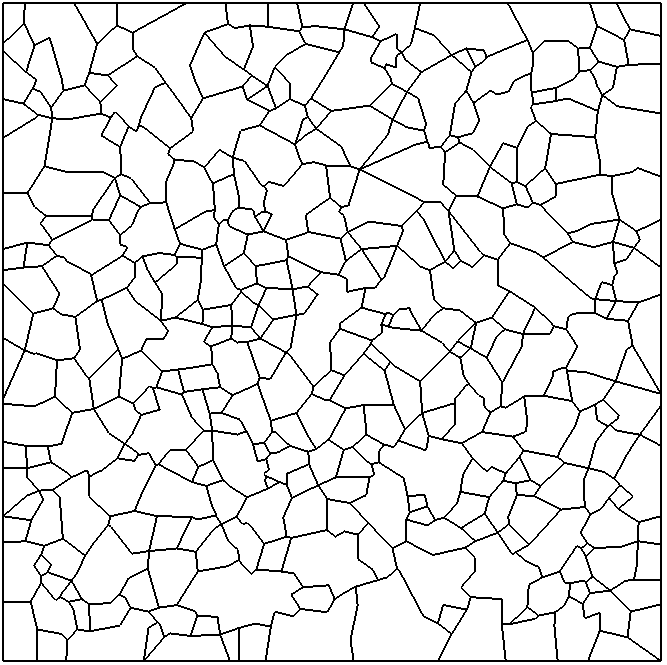
\includegraphics[width=0.4\textwidth]{1000points.png}} 
\subfigure[%Voronoi diagram
]{\label{fig:voromesh10000}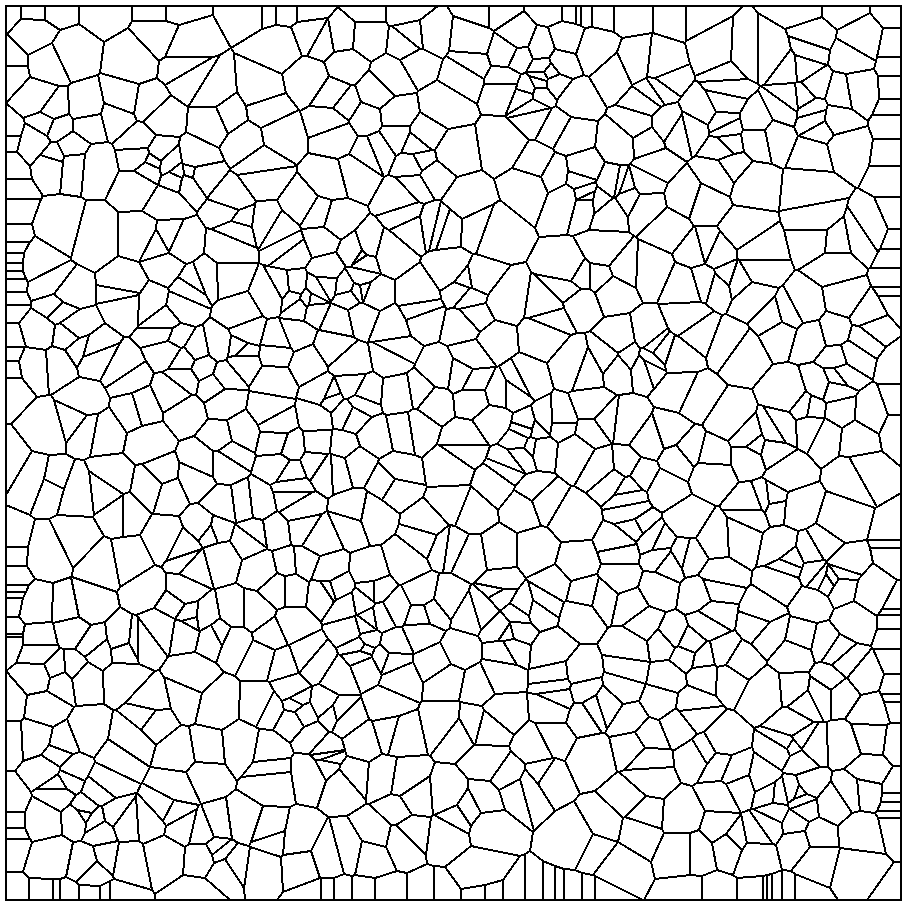
\includegraphics[width=0.4\textwidth]{voronoicomparision.png}}
\caption{Meshes generated from 1000 random points. (a) Polylla mesh.\textbf{(b)} Constrained Voronoi mesh generated with Detri2qt \cite{Detri2}. }
\label{figs:voro_comp} 
\end{figure}





\begin{figure}[]
\centering     %%% not \center
\subfigure[%Unicorn Triangulation
]{\label{fig:PSLGUnicornTriangulation}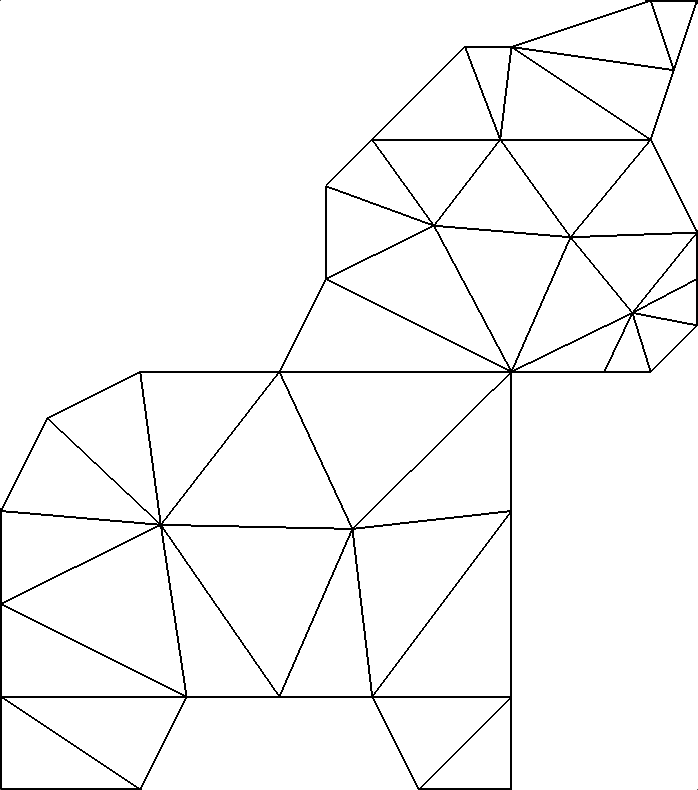
\includegraphics[width=0.25\textwidth]{unicorntriangulation.png}}%
\subfigure[%Unicorn Terminal-edge mesh
]{\label{fig:PSLGUnicorn}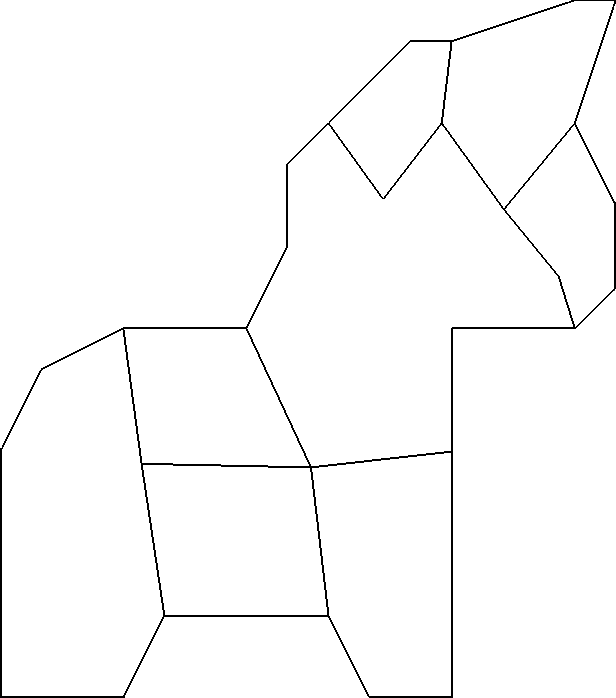
\includegraphics[width=0.25\textwidth]{unicorn.png}}%
\subfigure[%Clipped Voronoi unicorn
]{\label{fig:PSLGUnicornVoronoi}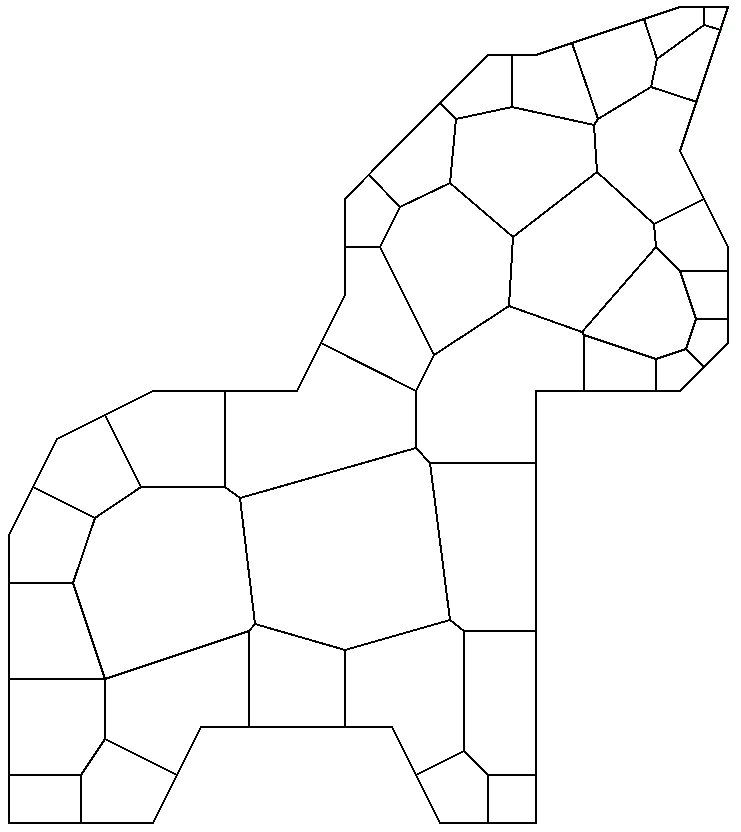
\includegraphics[width=0.25\textwidth]{voronoiunicord.png}}%
\subfigure[%Unicorn from more refined triangulation
]{\label{fig:PSLGUnicorn100}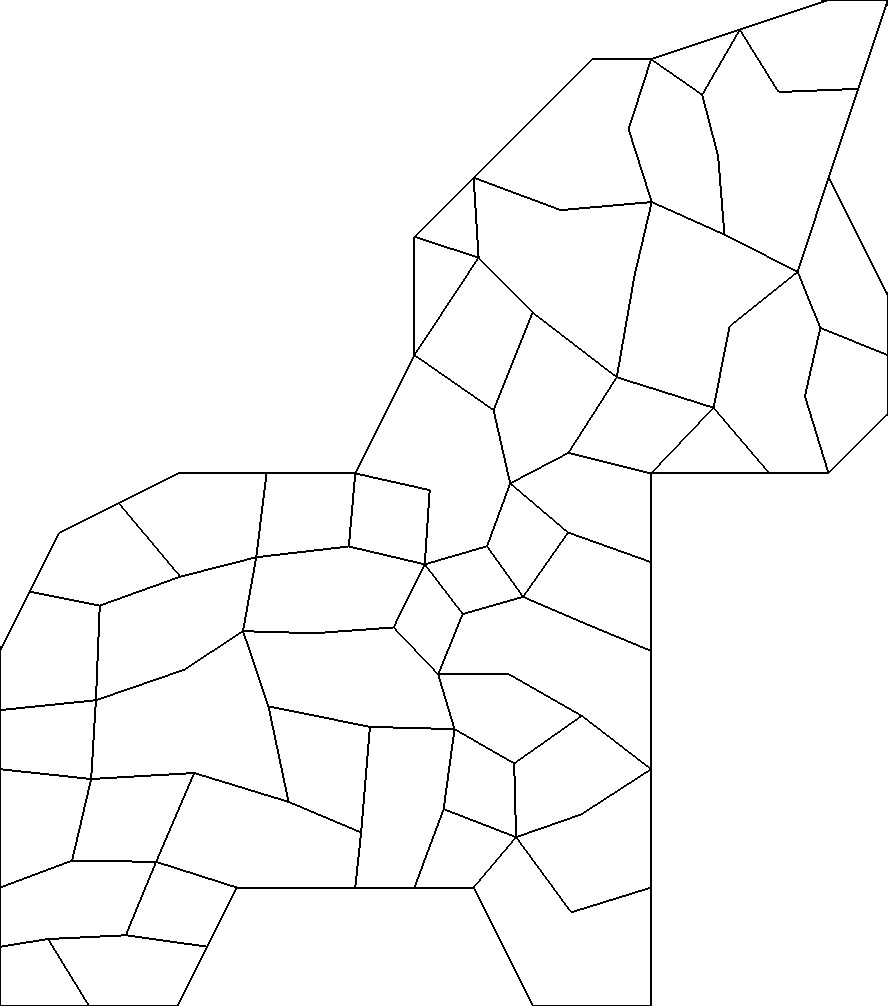
\includegraphics[width=0.25\textwidth]{unicorn100.png}}

\caption{ Qualitative comparison using an Unicorn PLSG as input \cite{AlejandroNUA2019} (a) Triangulation of unicorn PLSG with 36 vertices. (b) Polylla mesh includes exactly the 36 input vertices. (c) The constrained Voronoi mesh requires 100 vertices to model the same input. (d) Polylla mesh from a refined  Delaunay triangulation with 100 vertices.}
\label{figs:univornPSLG} 
\end{figure}



In Fig.~\ref{figs:voro_comp} a qualitative comparison between a Polylla mesh and a constrained Voronoi  mesh can be observed. Both meshes were generated from the same initial random point set. Fig.~\ref{fig:polymesh} shows the polygonal mesh generated by Polylla and Fig.~\ref{fig:voromesh10000} the constrained Voronoi mesh generated by Detri2qt. Some other examples of polygonal meshes generated for non convex domains are shown in Fig. \ref{figs:facePSLG} and Fig. \ref{figs:univornPSLG}.

 Fig. \ref{figs:univornPSLG} shows polygonal meshes for an Unicorn example generated by both  the Polylla  (Fig. \ref{fig:PSLGUnicorn}) and  Detri2qt (Fig. \ref{figs:univornPSLG}) tools. The initial triangulation and interior points are shown  in Fig. \ref{fig:PSLGUnicornTriangulation}. As expected, the  constrained Voronoi  mesh contains more points (100 vertices) and polygons than the Polylla mesh as shown in Fig. \ref{figs:univornPSLG}. Just for a qualitative comparison, we used Polylla to generate a polygonal mesh from 100 vertices and this mesh is shown in Fig. \ref{fig:PSLGUnicorn100}. 

%\textcolor{blue}{Fig.~\ref{figs:PSLG} shows example of the terminal-edge mesh with PLSG as input and a comparison with clipped Voronoi mesh. Fig. \ref{fig:PSLGface} is a classic PLSG from \cite{triangle2d} and Figures \ref{fig:PSLGUnicorn} and \ref{fig:PSLGUnicorn2} are PLSG from~\cite{AlejandroNUA2019}, both Figures have 36 vertices as input, but the Fig. \ref{fig:PSLGUnicorn2} has in total 100 vertices as output. }

%Fig. \ref{fig:PSLGface} is a PLSG obtained from~\cite{triangle2d} and Figures \ref{fig:AlejandroNUA2019} a is a PLSG obtained in from~\cite{ale}, both use the same number of vertices as the initial triangulation used by their generation, but Fig. \ref{fig:PSLGface} added other 64 vertices to constrain the Voronoi cells inside the geometric domain.

%As an example of initial polygonal meshes polygonal meshes generated from PLSG geometries are shown in Fig. . 


\section{Preliminary Simulation Results}
\label{sec:simulation_results}
In this section, we assess the Polylla meshes using the virtual element method (VEM)~\cite{Basisprinciples}. To this end, an L-shaped domain is considered. Fig.~\ref{figs:LshapedPolylla} shows this domain meshed with a random and a semiuniform Polylla sample mesh. For comparison purposes, we also consider random and semiuniform Voronoi meshes (sample meshes are depicted in Fig.~\ref{figs:LshapedVoronoi}). The chosen problem is governed by the Laplace equation and its exact solution is given by~\cite{MITCHELL2013350}
\begin{equation*}
u(x_1,x_2)=r^{2/3} \sin(2/3\,\theta), \quad r=\sqrt{x_1^2+x_2^2}, \quad \theta(x_1,x_2)=\arctan(x_2/x_1).
\end{equation*}



The boundary conditions are of Dirichlet type with the exact solution imposed on the entire domain boundary. The re-entrant corner of the L-shaped domain introduces a singularity in the solution that manifests  itself as unbounded derivatives of $u$ at the origin. The numerical solution (denoted by $u_h$) is assessed  through its convergence with mesh refinements. Figs.~\ref{figs:NormsLshapedRandom} and 
\ref{figs:NormsLshapedSemiuniform} present the $L^2$ norm and the $H^1$ seminorm of the error, where it is shown that the VEM on Polylla (random and semiuniform) and Voronoi (random and semiuniform) meshes delivers accurate solutions with optimal convergence rates of 2 (for the $L^2$ norm) and 1 (for the $H^1$ seminorm).

The performance of VEM using Polylla (random and semiuniform) and Voronoi (random and semiuniform) meshes are compared in Fig.~\ref{figs:PerformanceLshaped}, where the $H^1$ seminorm of the error and the normalized CPU time are each plotted as a function of the number of degrees of freedom (DOF). The normalized CPU time is defined as the ratio of the CPU time of a particular simulation to the maximum CPU time found for any of the simulations that were run. Each of the four set of meshes (random Polylla, semiuniform Polylla, random Voronoi and semiuniform Voronoi) consists of four meshes of increasing number of degrees of freedom. Therefore, in total, there are sixteen meshes in the study. 

The CPU time is measured from the reading of the mesh until the solution of the system of equations is ended. Each mesh is run ten times and the CPU time recorded is the average CPU time. From Fig.~\ref{figs:PerformanceLshaped} it is observed that for equal number of degrees of freedom similar accuracy and computational cost are obtained for the four set of meshes.

Finally, for completeness of the presented numerical results, contour plots of the VEM solution on Polylla meshes are shown in Figs.~\ref{figs:ContourPlots} and~\ref{figs:ContourPlotsGrad} for the $u_h$ and $\bm{\nabla}u_h$ fields, respectively.

\begin{figure}[!bth]
\centering     %%% not \center
\subfigure[]{\label{fig:LshapedPolyllaRandom}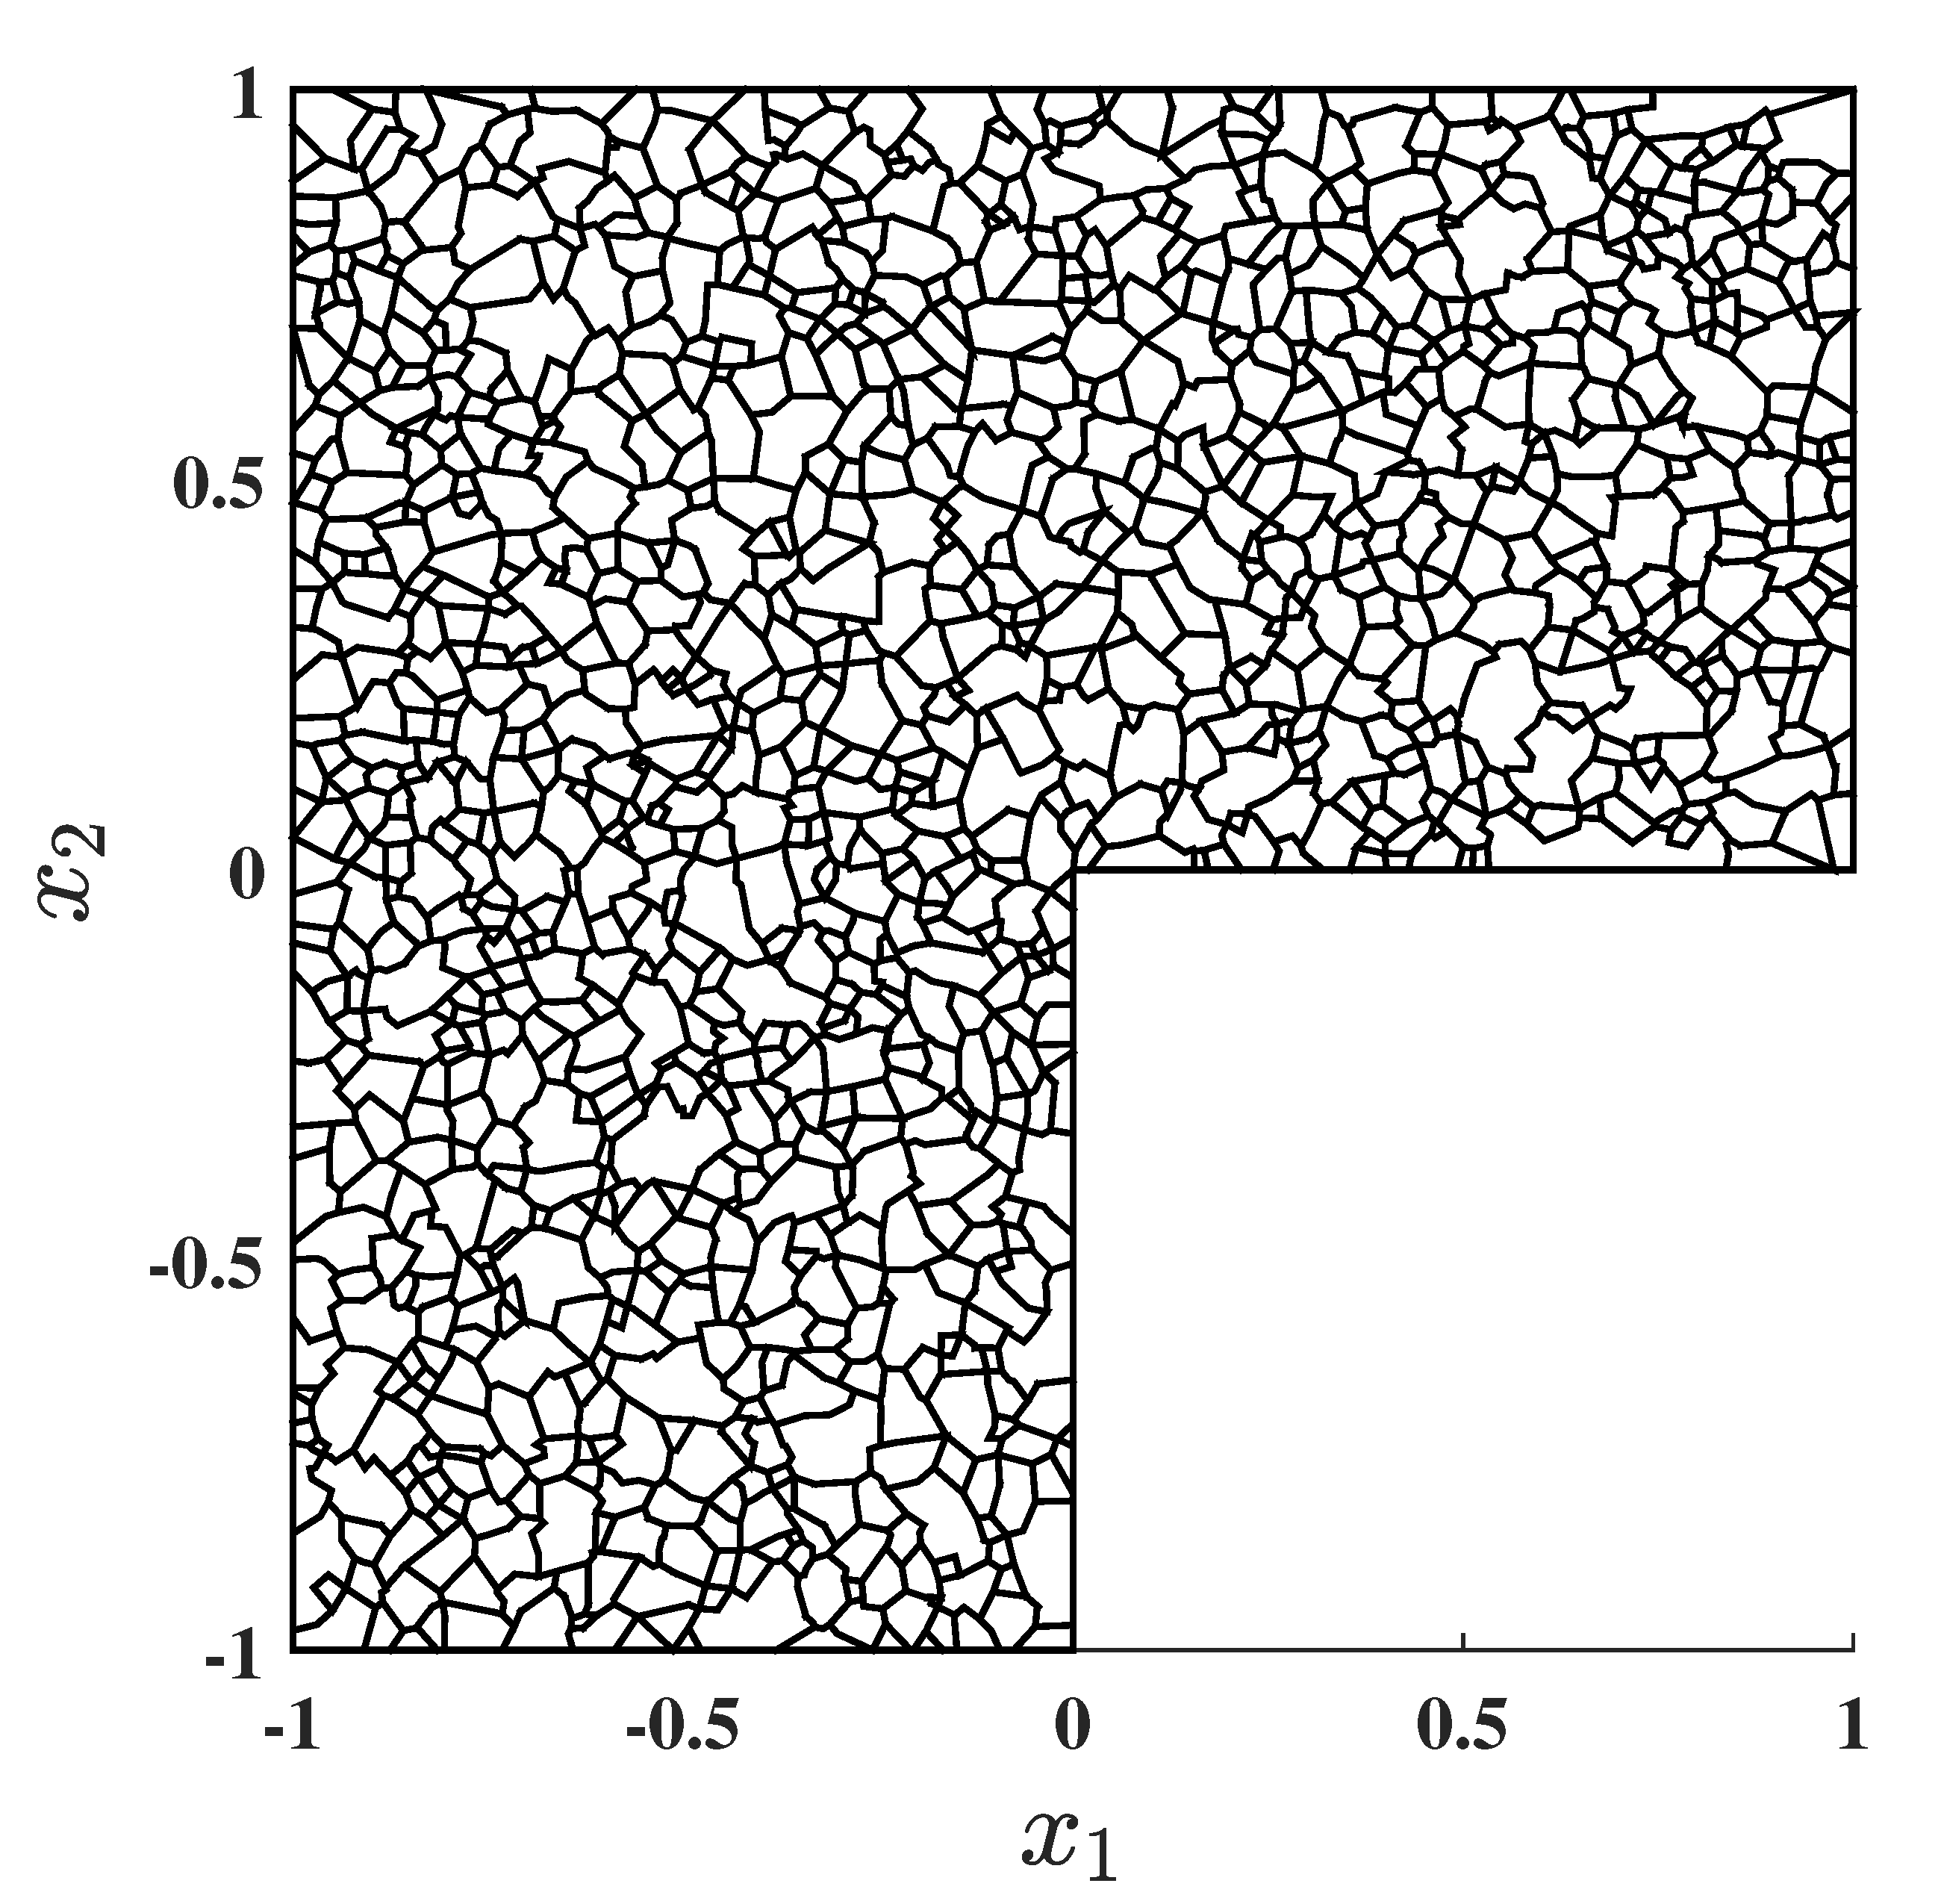
\includegraphics[width=0.4\textwidth]{Lshaped_polylla_random.png}} \hspace{0.1cm}
\subfigure[]{\label{fig:LshapedPolyllaSemiuniform}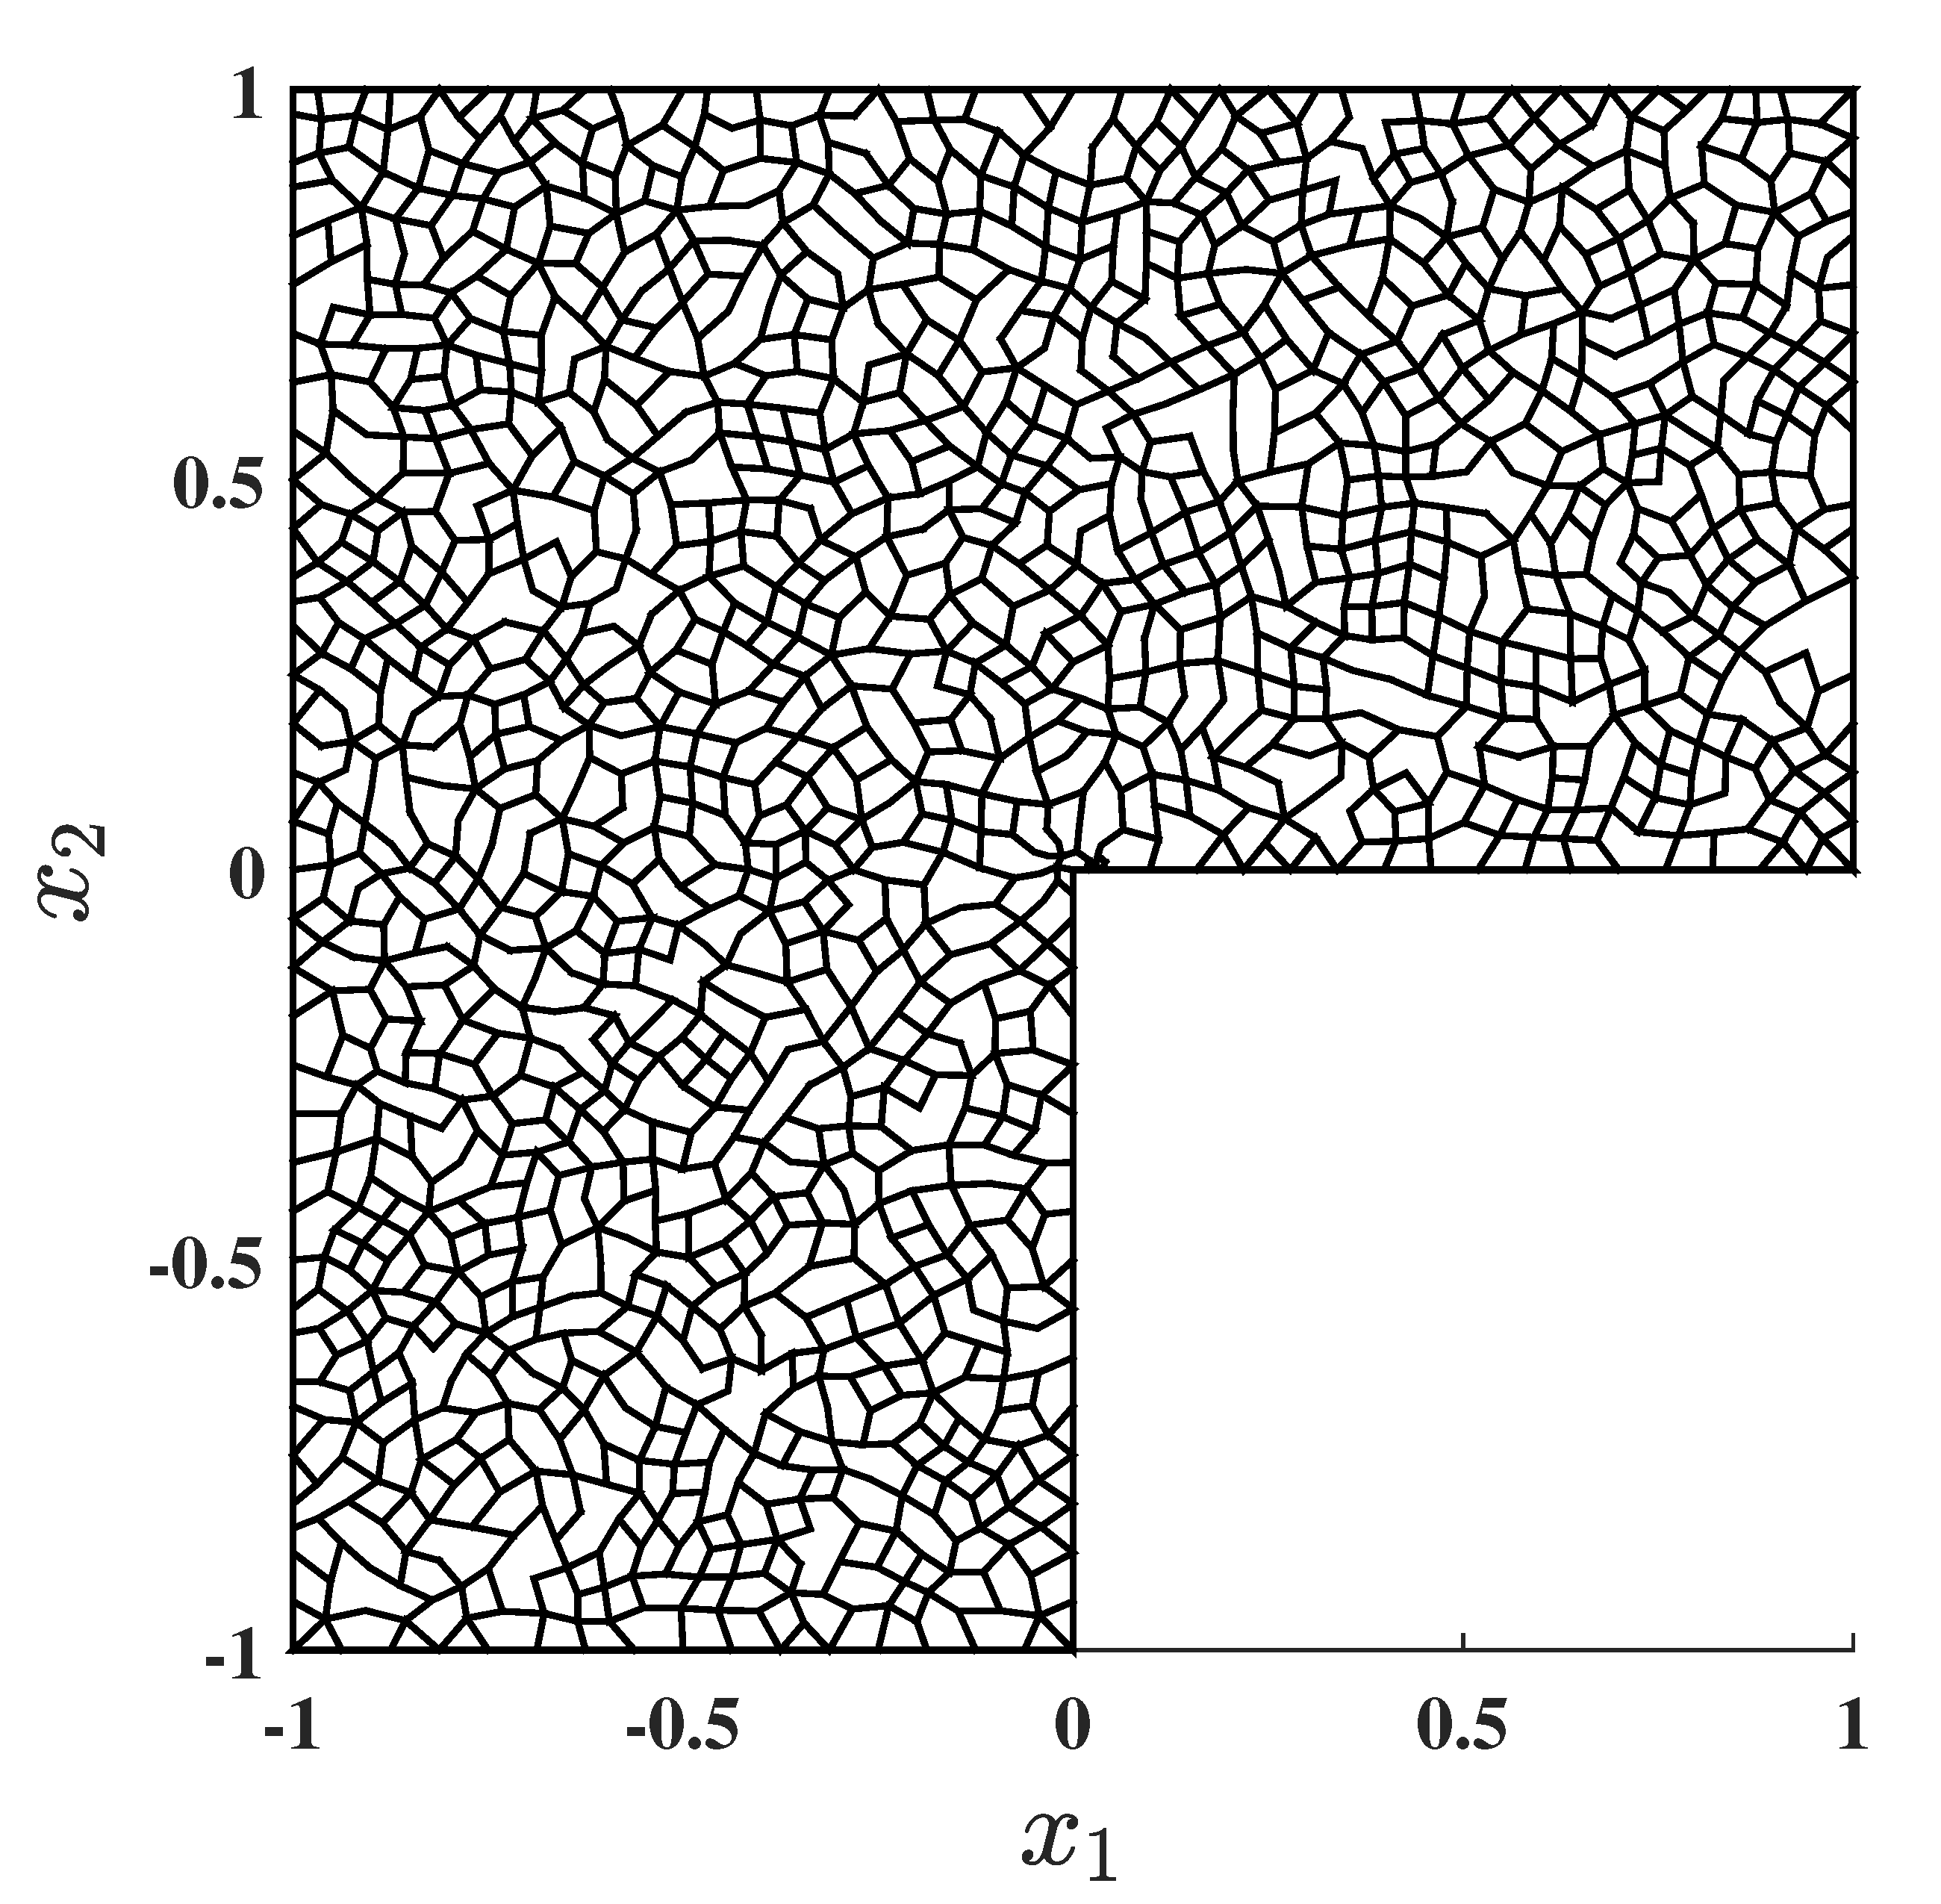
\includegraphics[width=0.4\textwidth]{Lshaped_polylla_semiuniform.png}}
\caption{L-shaped domain meshed with \textbf{(a)} a random and \textbf{(b)} a semiuniform Polylla mesh.}
\label{figs:LshapedPolylla} 
\end{figure}

\begin{figure}[!bth]
\centering     %%% not \center
\subfigure[]{\label{fig:LshapedVoronoiRandom}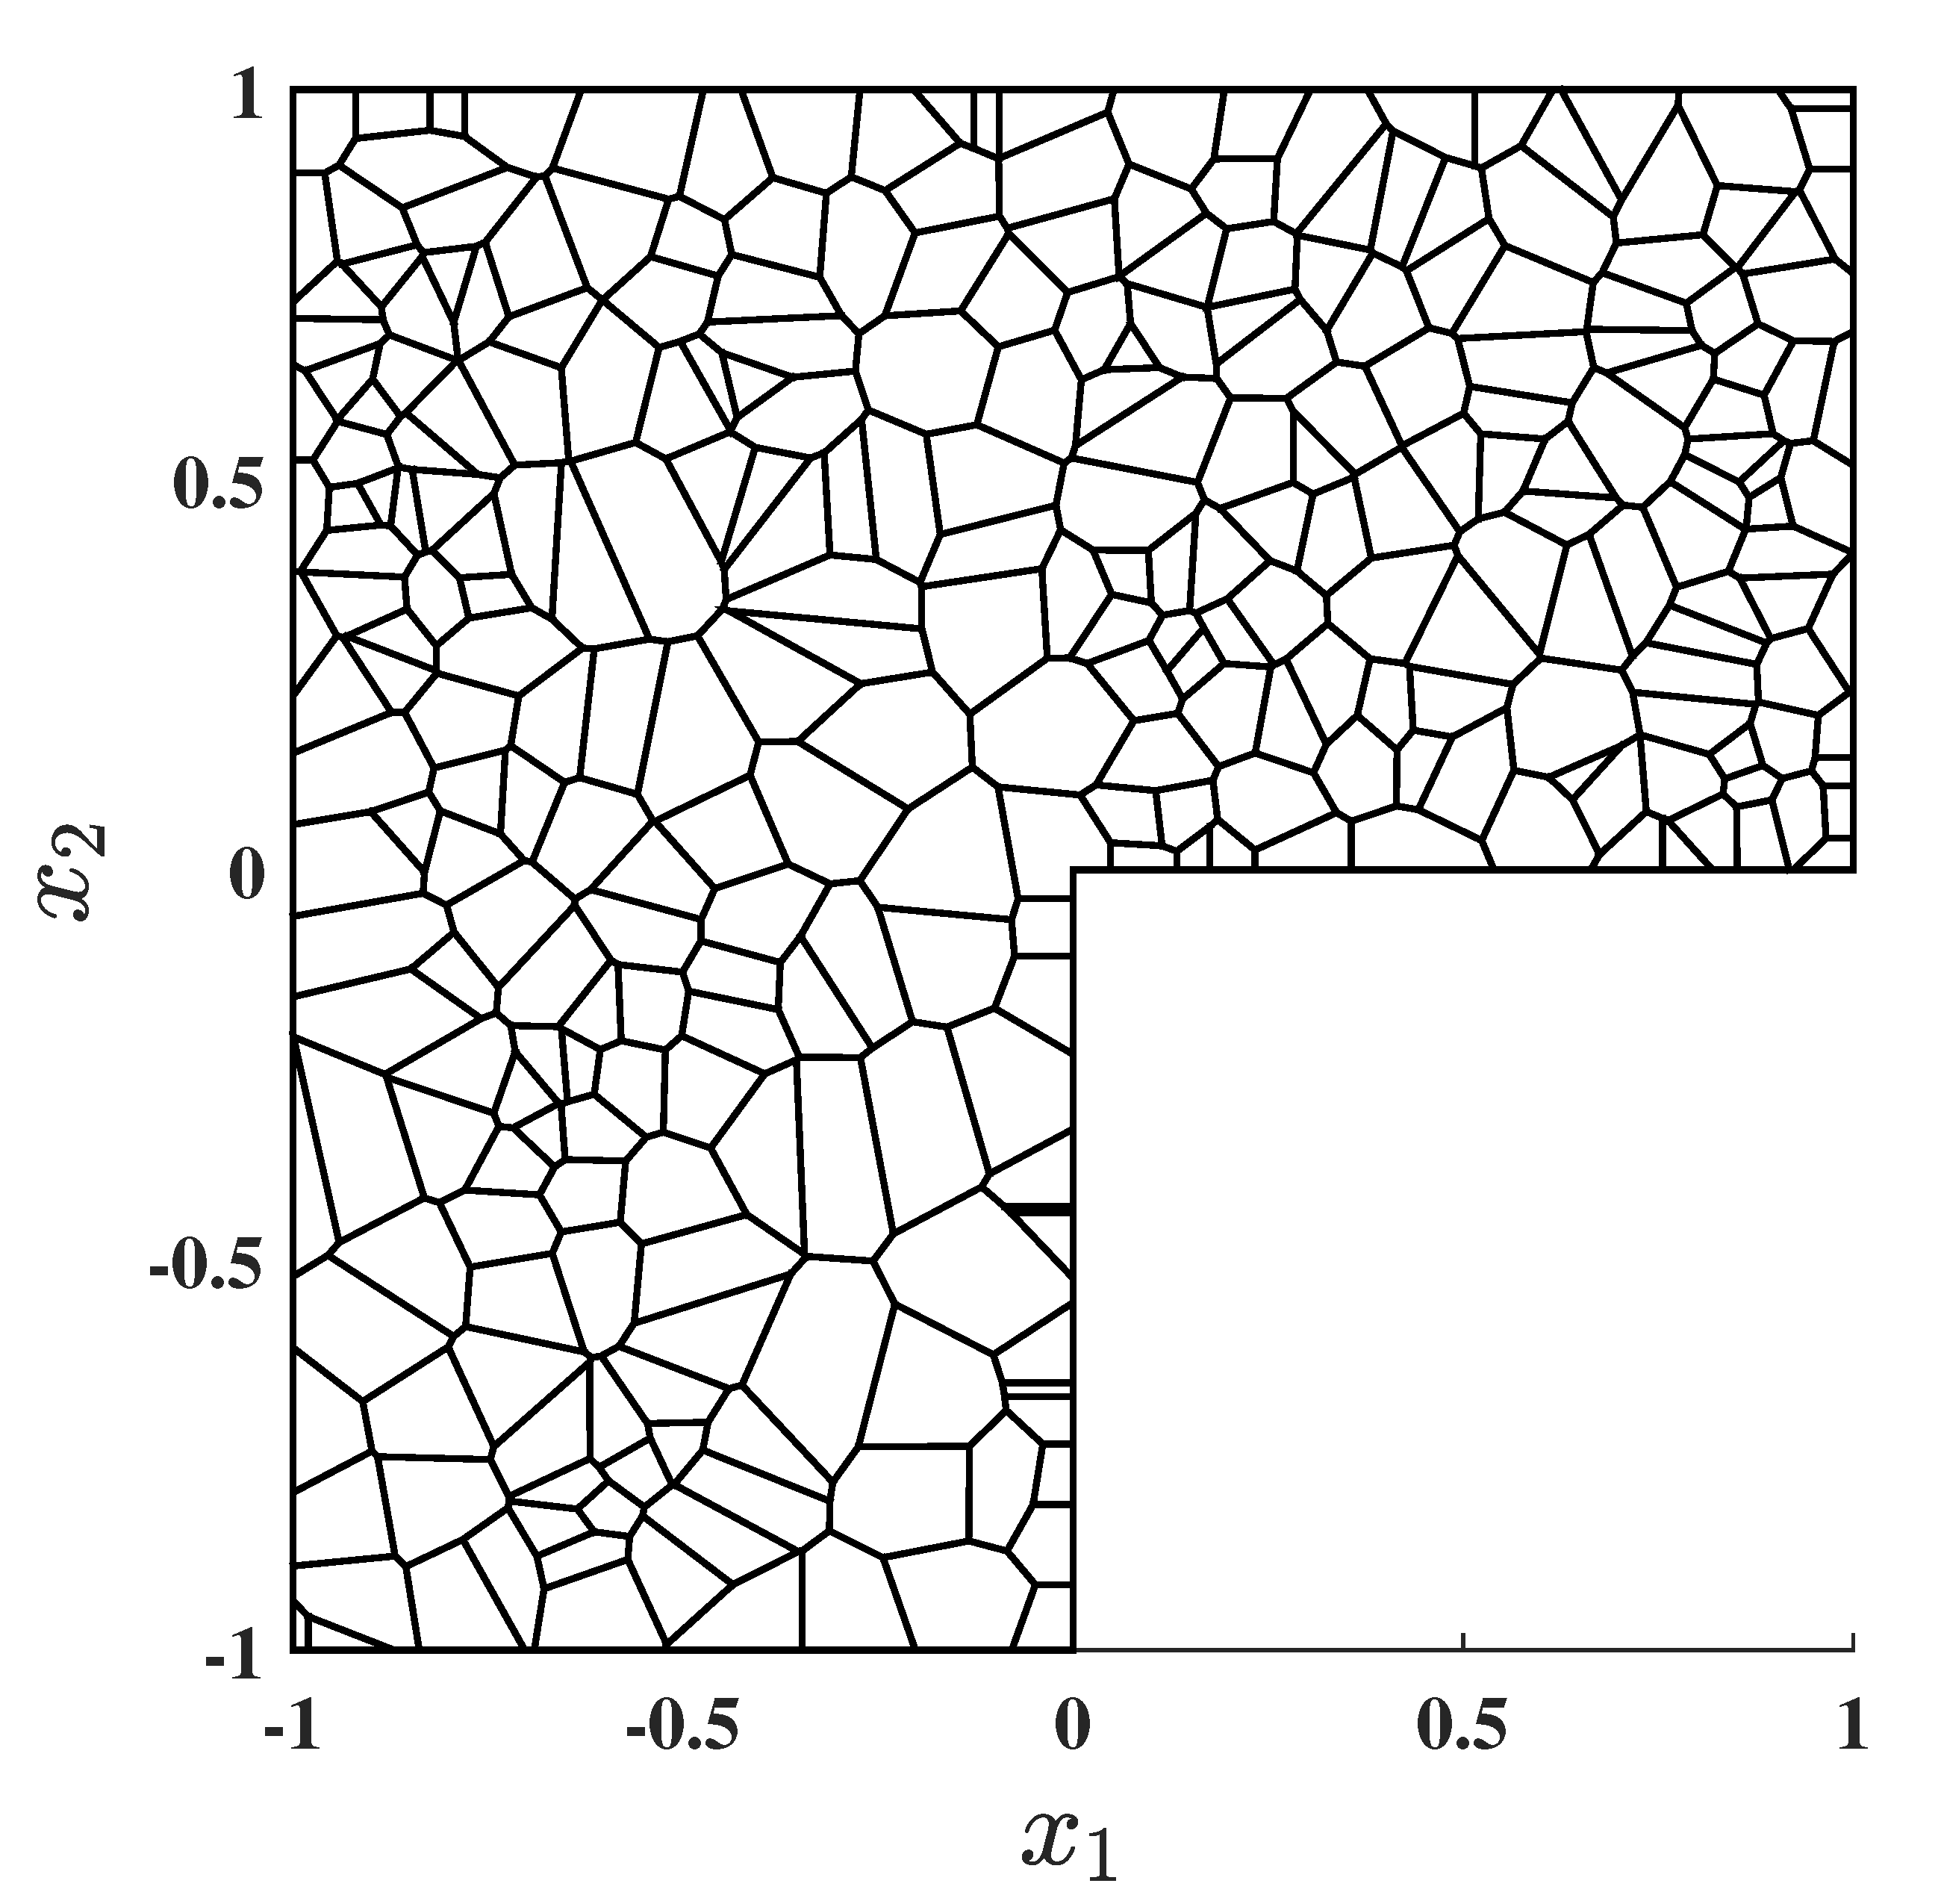
\includegraphics[width=0.4\textwidth]{Lshaped_voronoi_random.png}} \hspace{0.1cm}
\subfigure[]{\label{fig:LshapedVoronoiSemiuniform}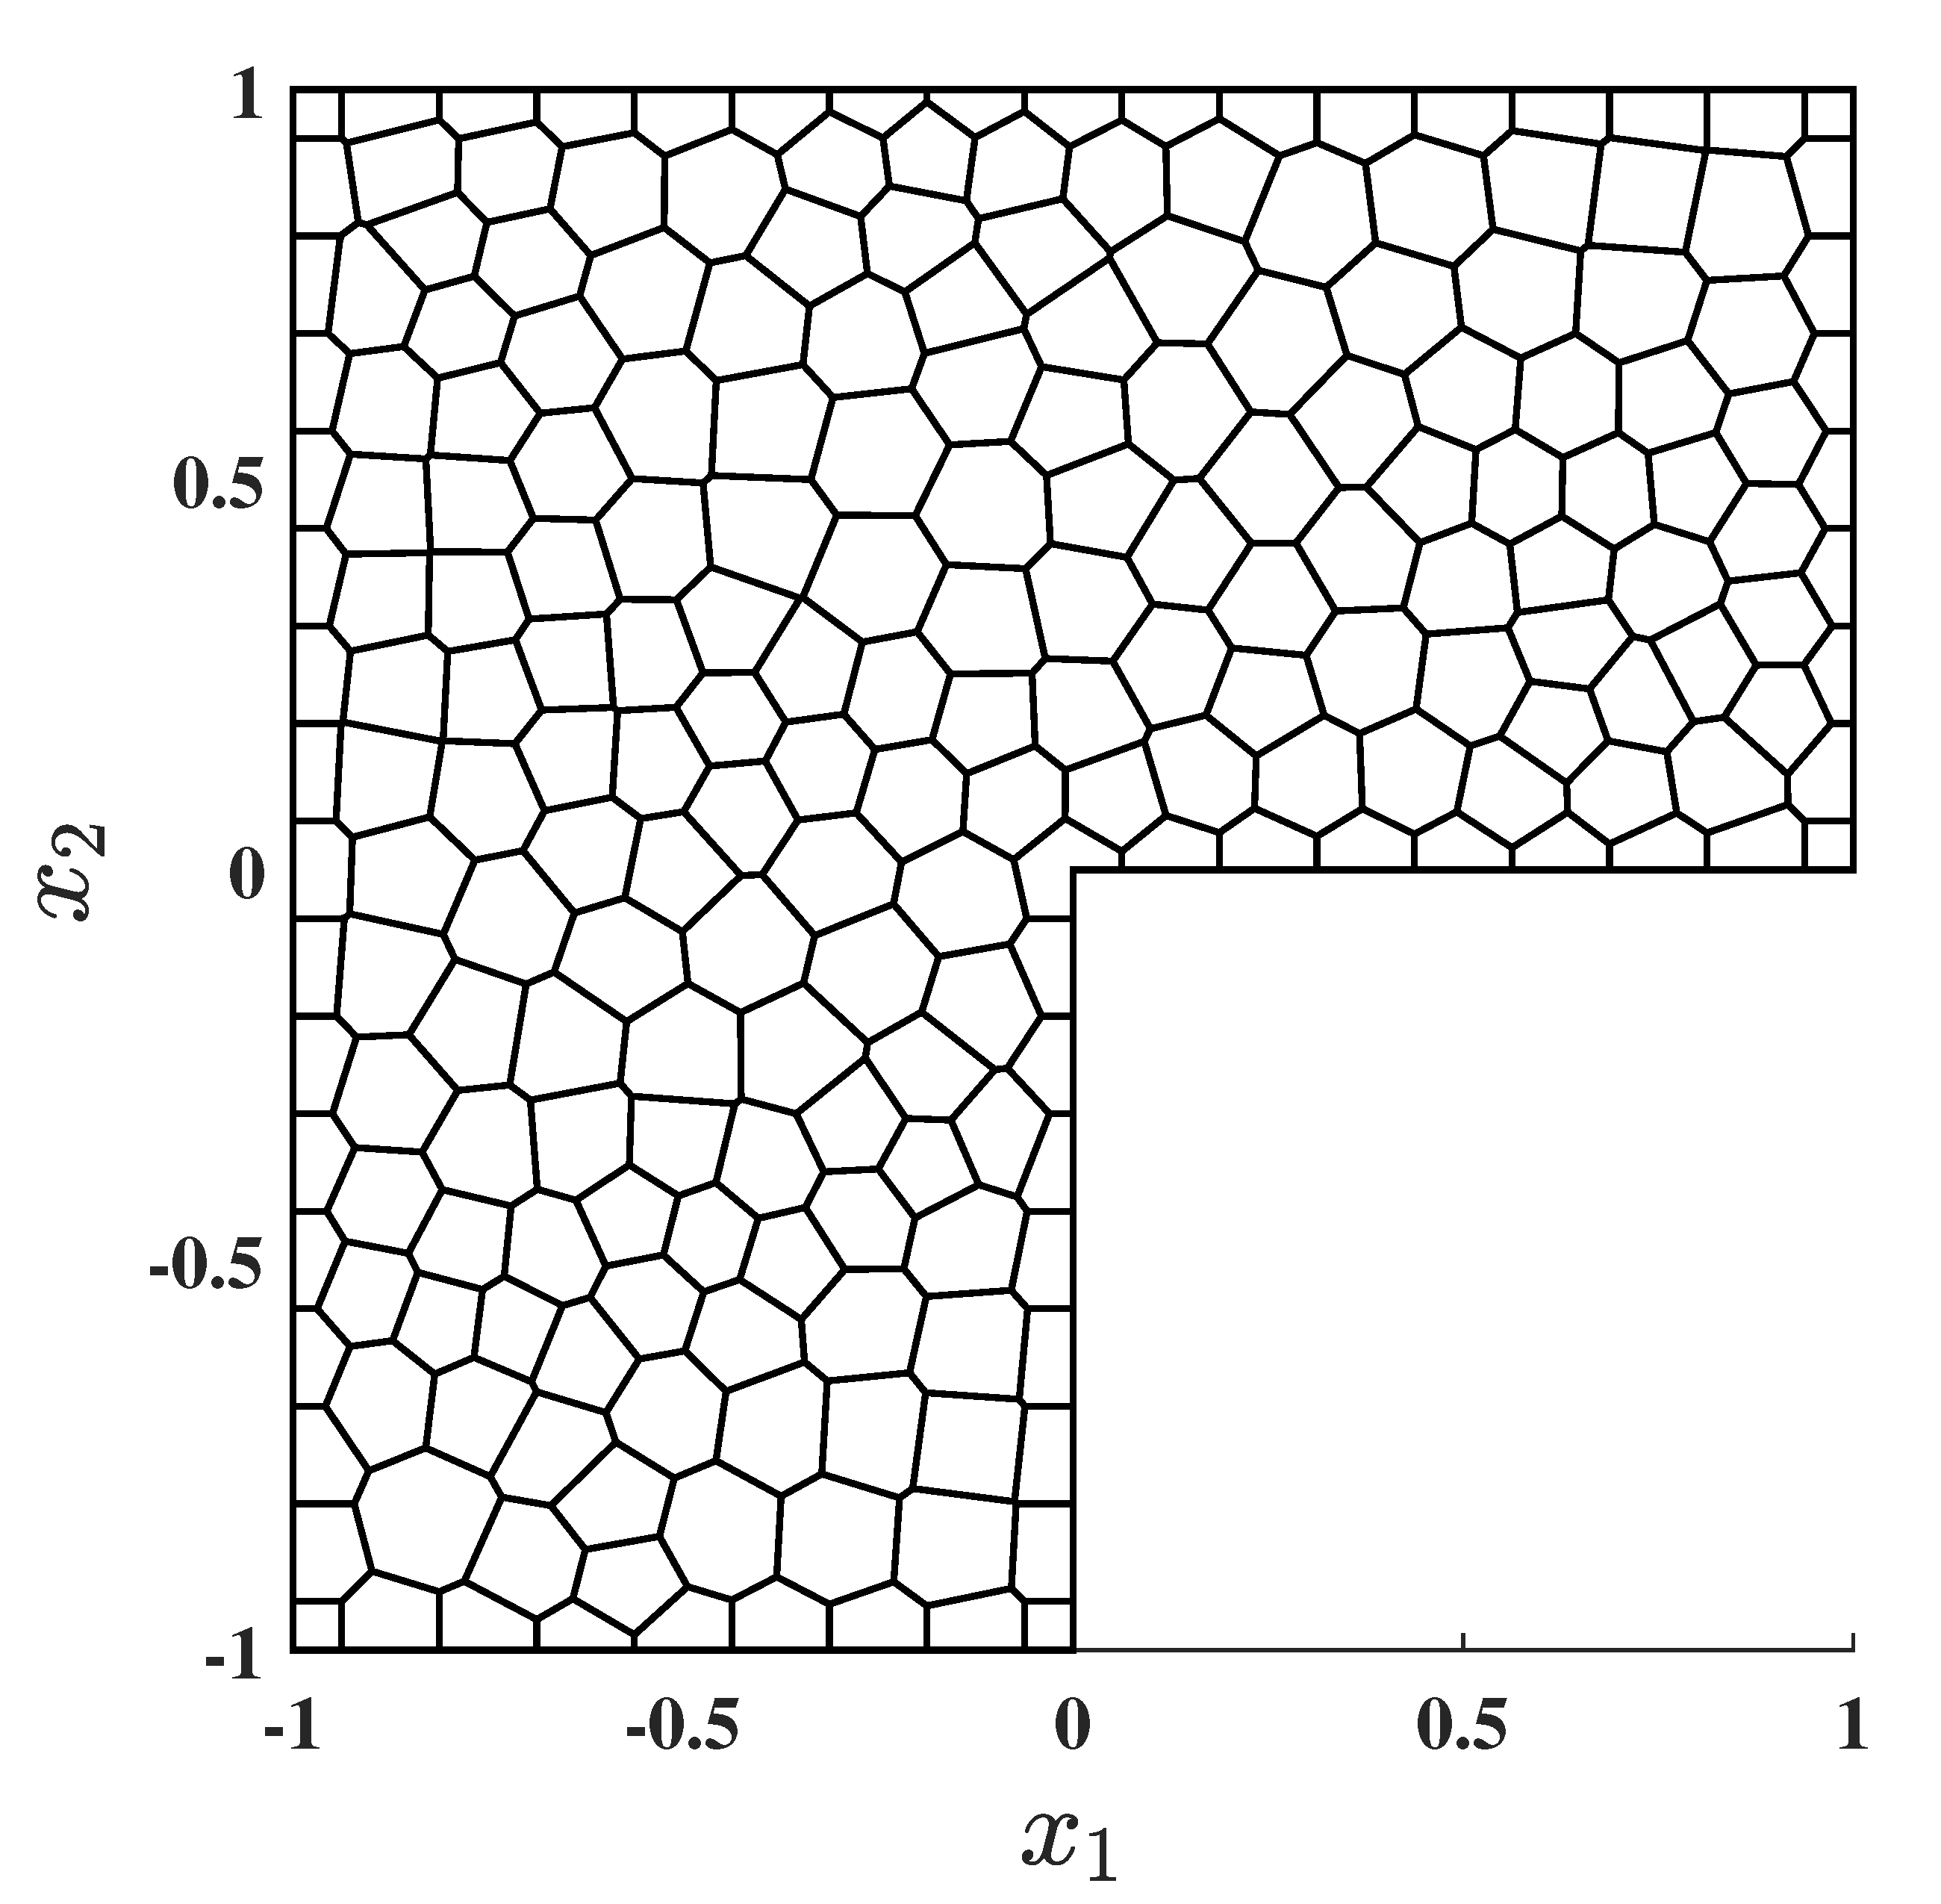
\includegraphics[width=0.4\textwidth]{Lshaped_voronoi_semiuniform.png}}
\caption{L-shaped domain meshed with \textbf{(a)} a random and \textbf{(b)} a semiuniform Voronoi mesh.}
\label{figs:LshapedVoronoi} 
\end{figure}

Note that random Polylla meshes (Fig~\ref{fig:LshapedPolyllaRandom}) were generated from constrained Delaunay triangulation built over  a L-shaped domain with points randomly generated in its interior. Semiuniform Polylla (Fig~\ref{fig:LshapedPolyllaSemiuniform}) meshes were generated  from a conforming Delaunay triangulation using pygalmesh~\cite{Schlomer_pygalmesh_Python_interface}. To generate the same number of triangles as the random mesh, an arbitrary maximum edge size constraint was given as input.  The random (Fig~\ref{fig:LshapedVoronoiRandom}) and semiuniform (Fig~\ref{fig:LshapedVoronoiSemiuniform}) Voronoi meshes were generated from  the points (sites) of both the  constrained Delaunay triangulation and the conforming Delaunay triangulation, respectively. Next, each infinite Voronoi region was intersected with the L-shaped domain to generate the constrained Voronoi mesh.





\begin{figure}[!bth]
\centering     %%% not \center
\mbox{
\subfigure[]{\label{fig:L2LshapedPolyllaRandom}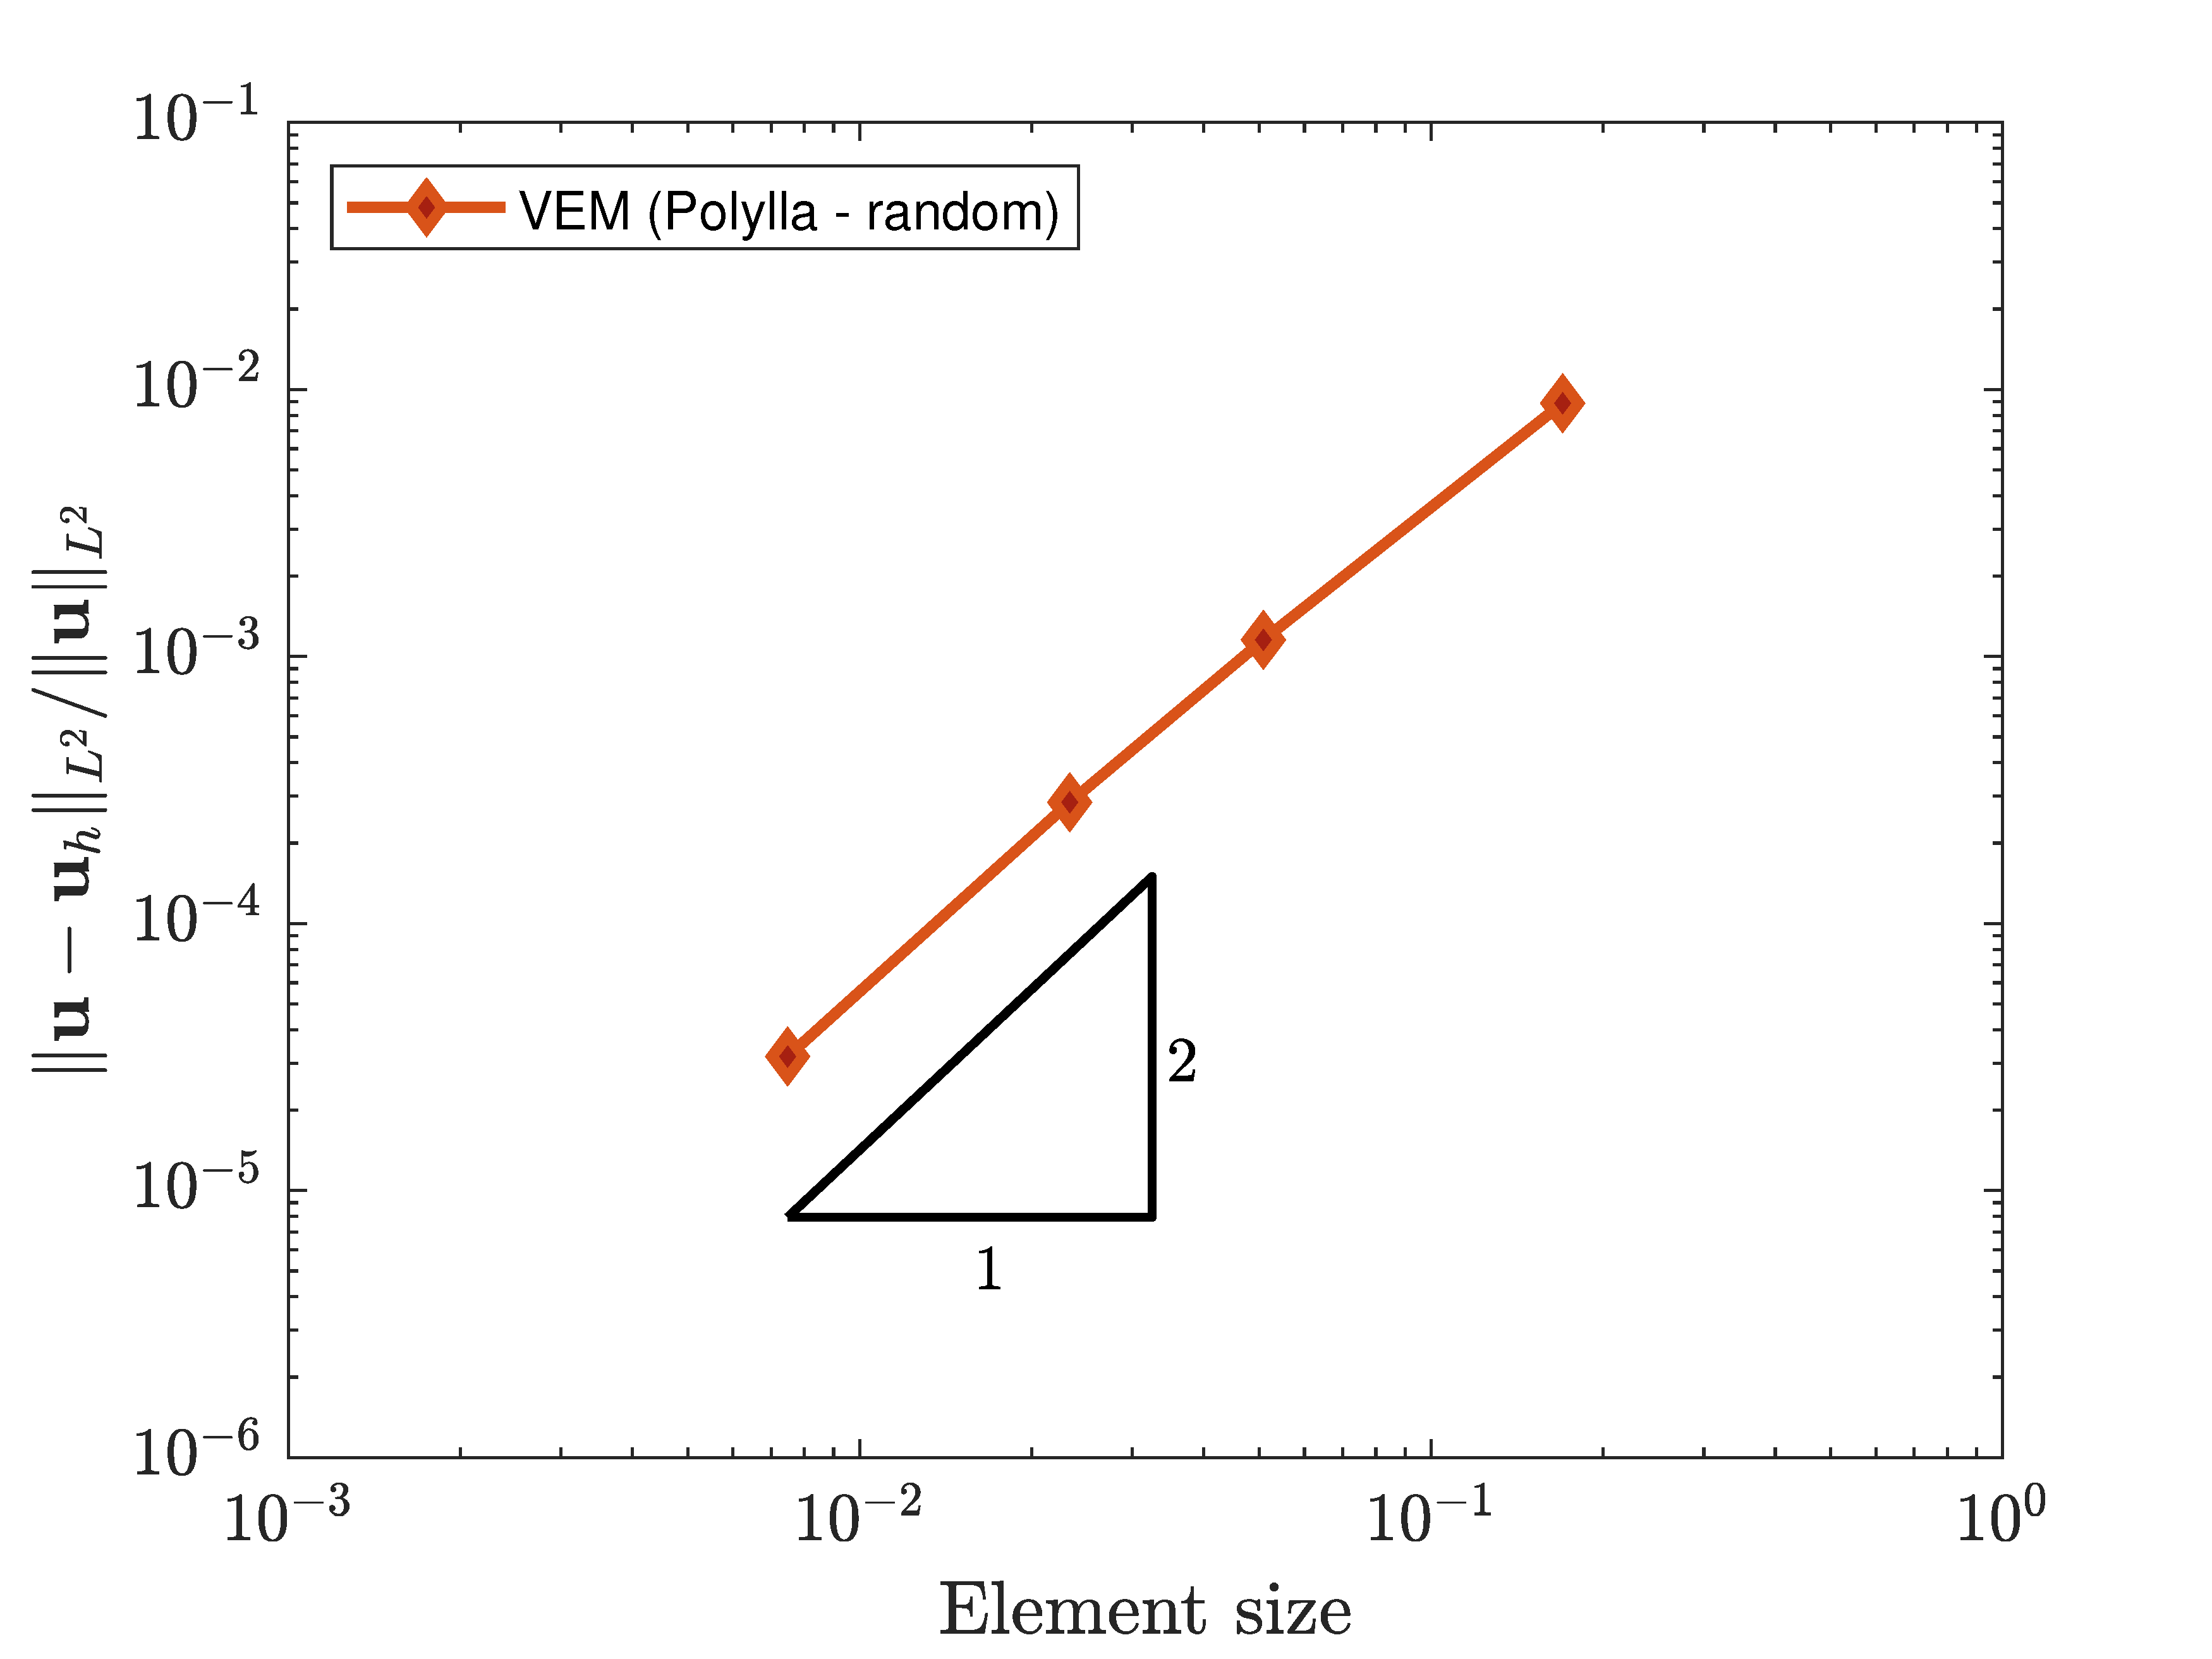
\includegraphics[width=0.4\textwidth]{L2_polylla_random.png}} \hspace{0.1cm}
\subfigure[]{\label{fig:H1LshapedPolyllaRandom}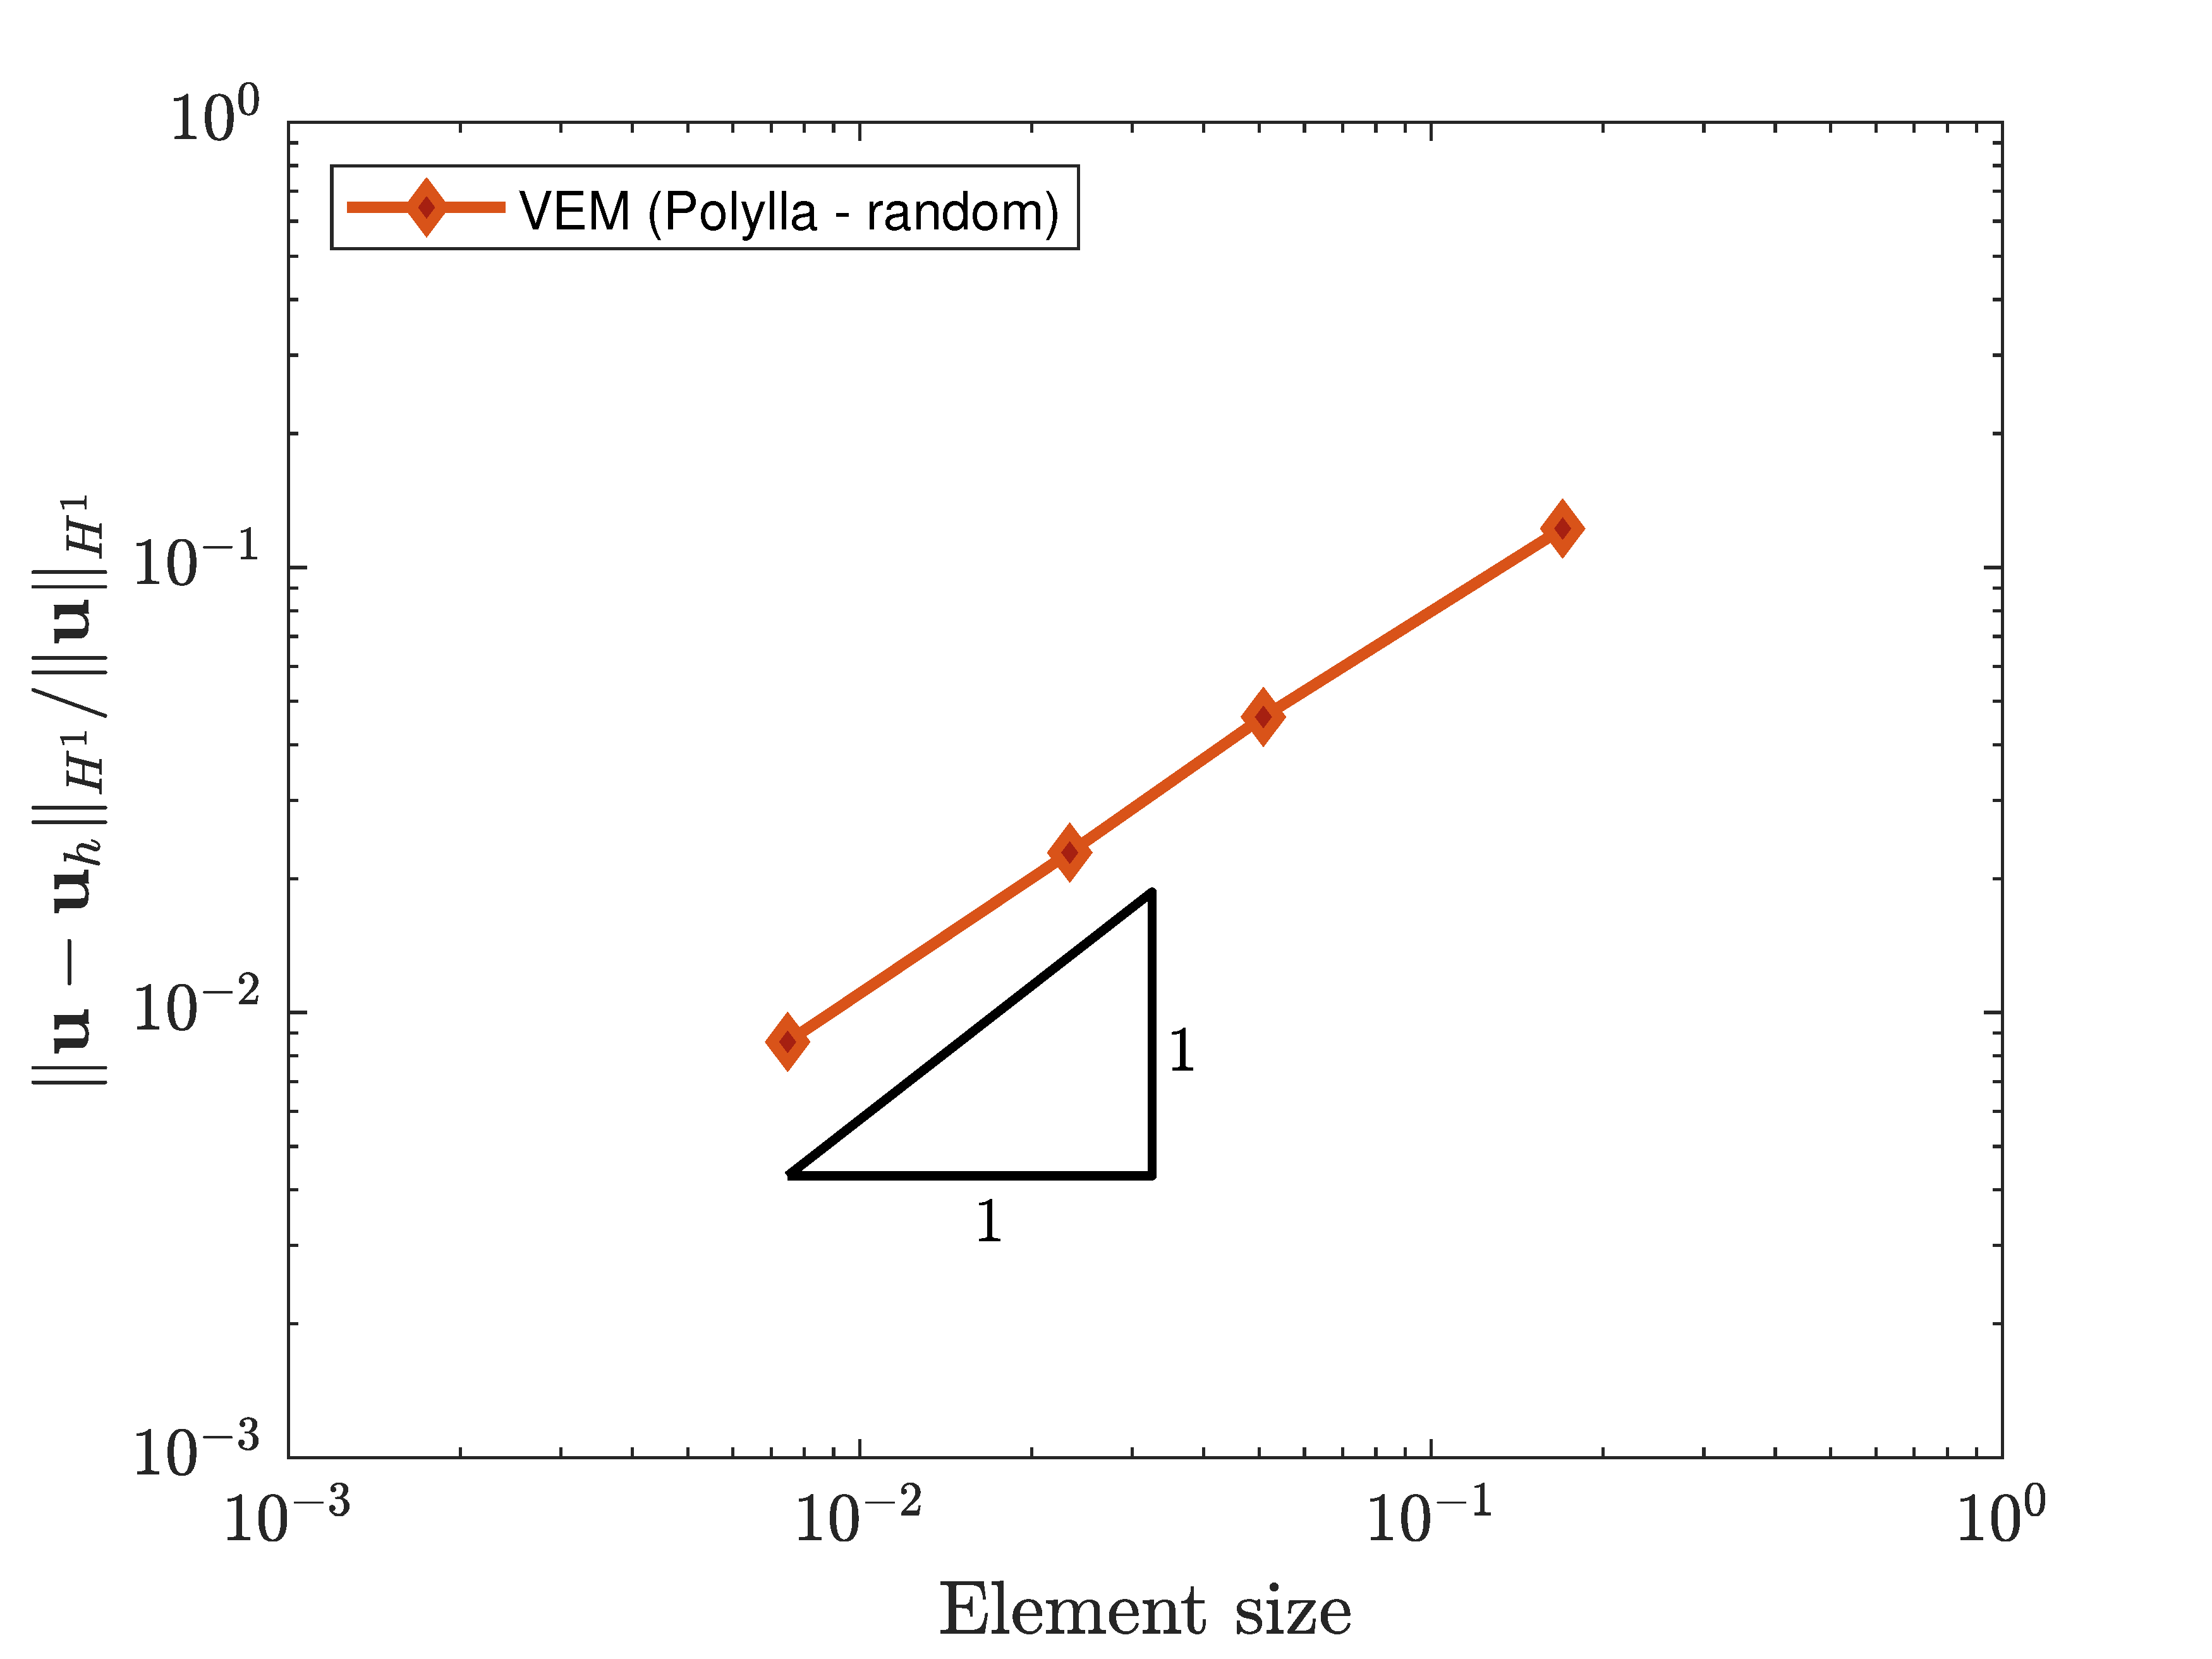
\includegraphics[width=0.4\textwidth]{H1_polylla_random.png}}
}
\mbox{
\subfigure[]{\label{fig:L2LshapedVoronoiRandom}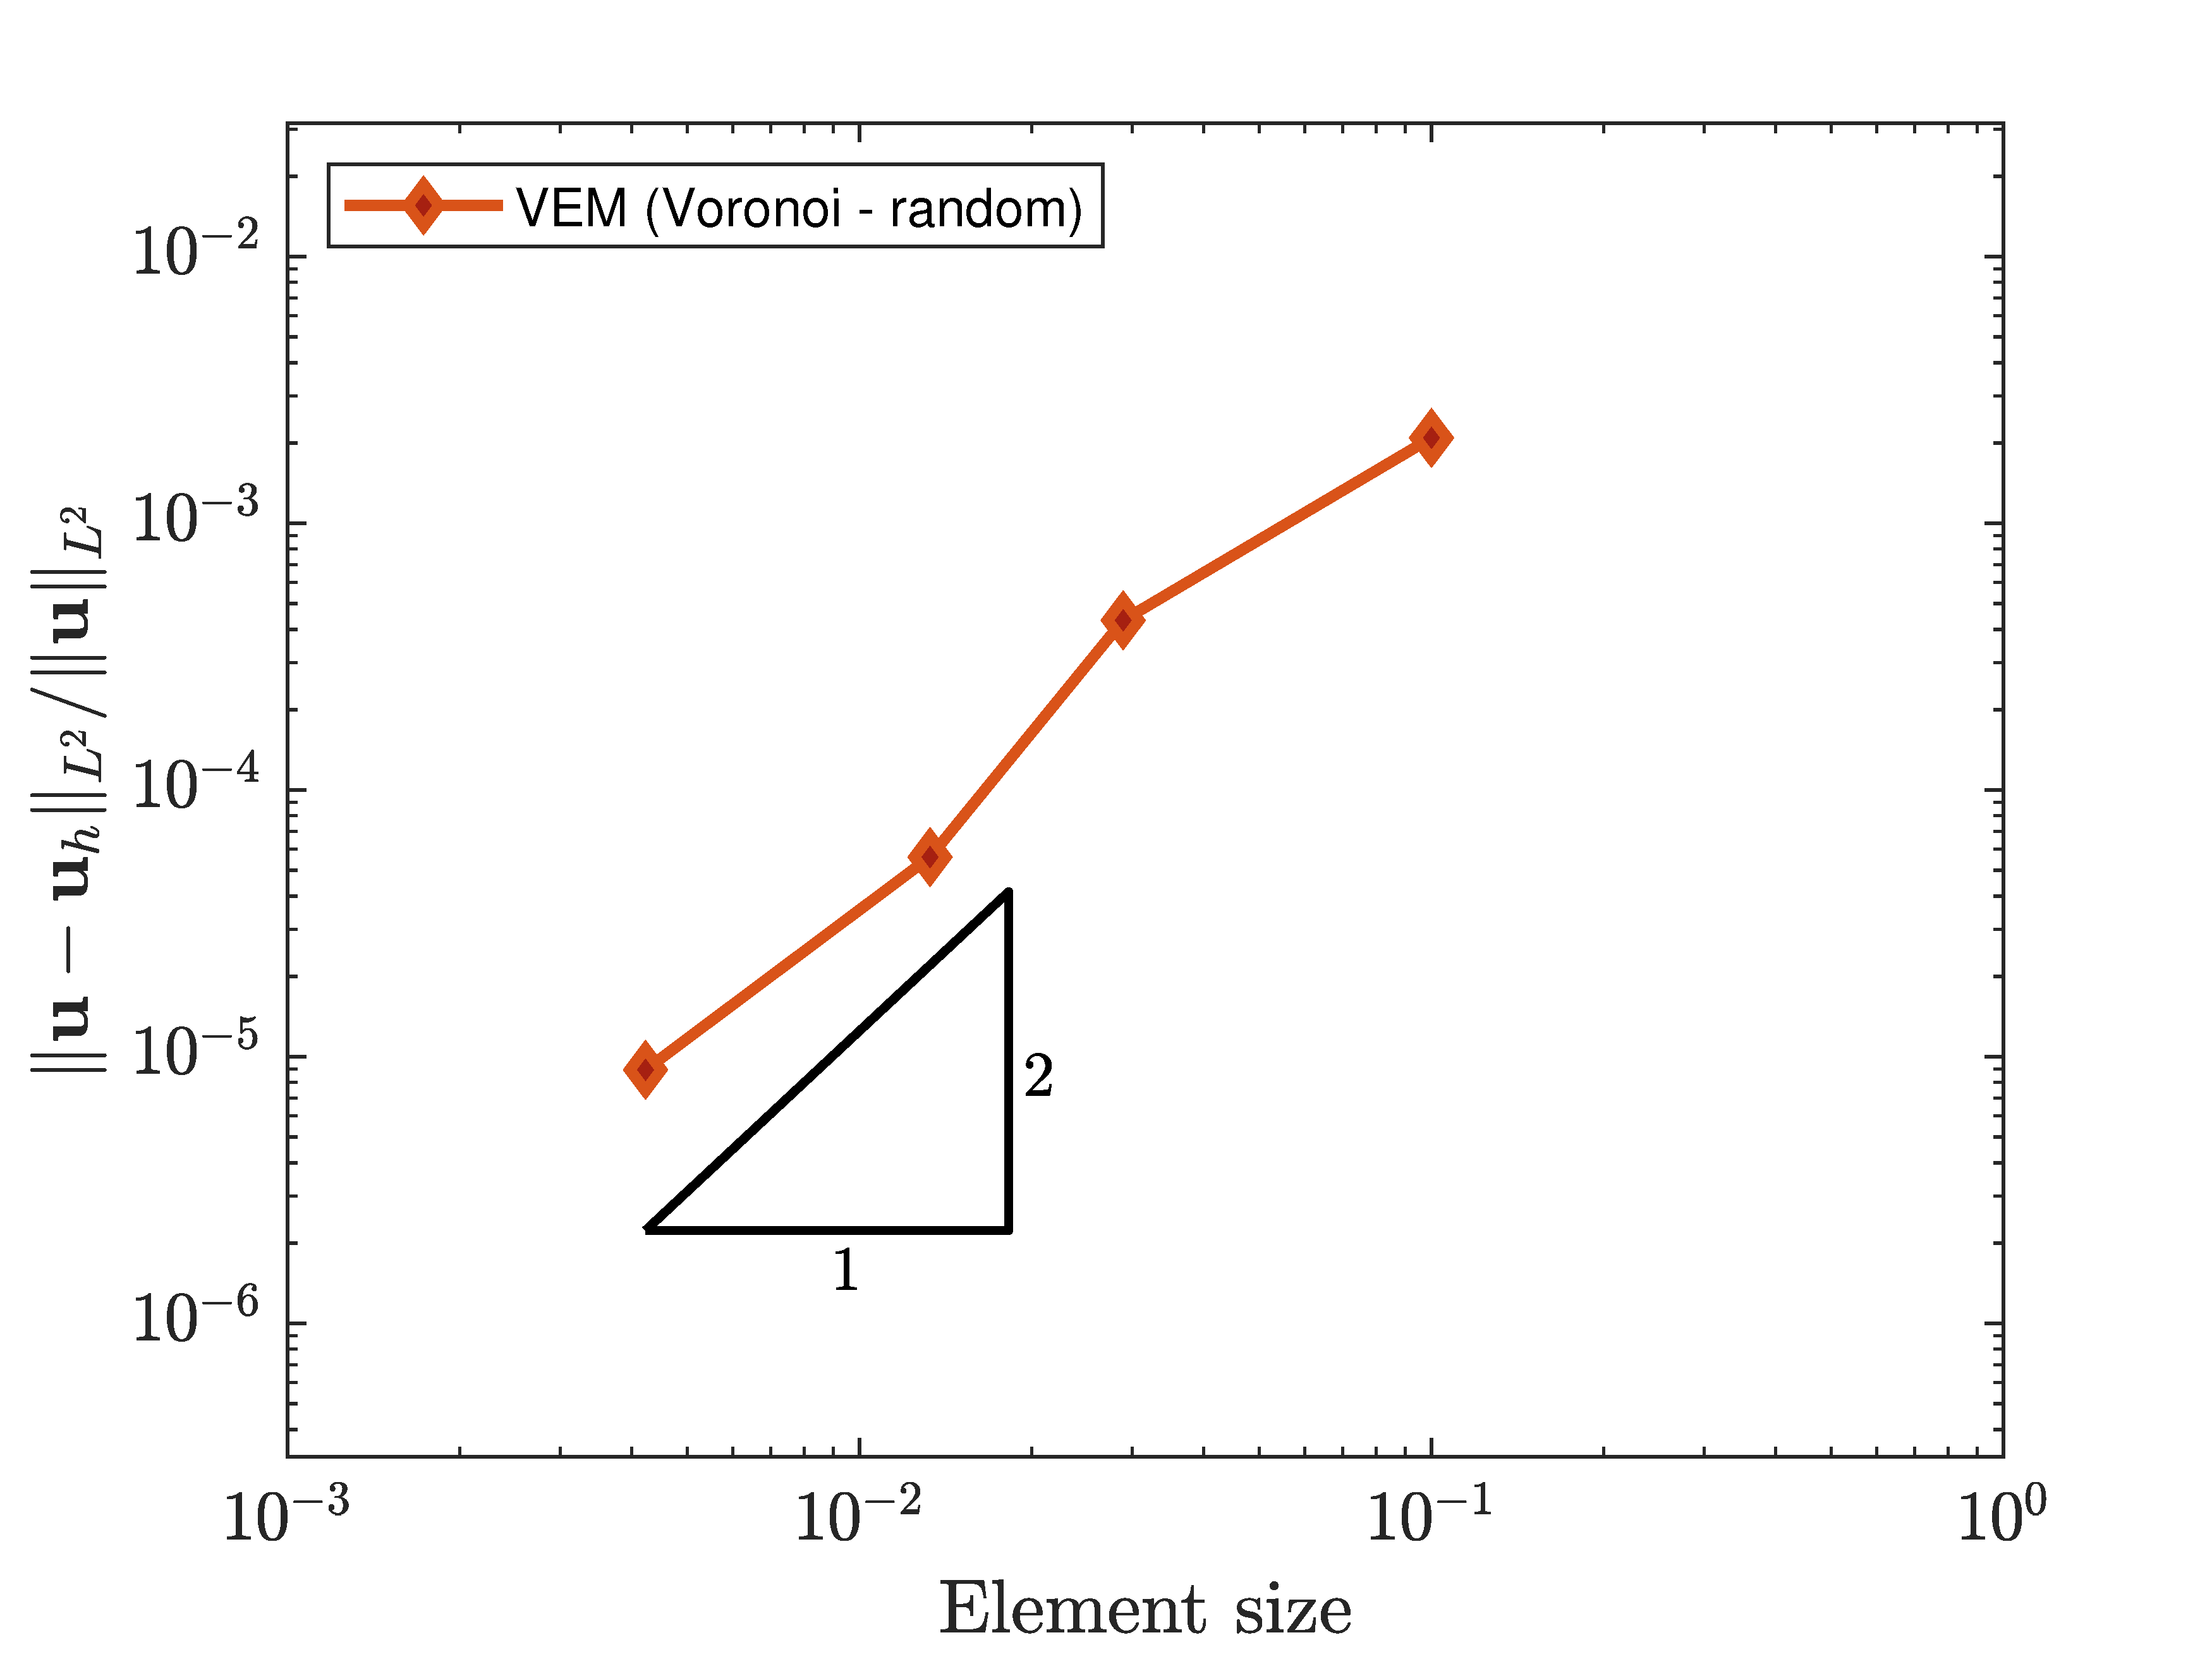
\includegraphics[width=0.4\textwidth]{L2_voronoi_random.png}} \hspace{0.1cm}
\subfigure[]{\label{fig:H1LshapedVoronoiRandom}\includegraphics[width=0.4\textwidth]{H1_voronoi_random.png}}
}
\caption{$L^2$ norm and $H^1$ seminorm of the error using the VEM on random Polylla meshes (\textbf{(a)} and \textbf{(b)}, 
respectively), and on random Voronoi meshes (\textbf{(c)} and \textbf{(d)}, respectively).}
\label{figs:NormsLshapedRandom} 
\end{figure}

\begin{figure}[!bth]
\centering     %%% not \center
\mbox{
\subfigure[]{\label{fig:L2LshapedPolyllaSemiuniform}\includegraphics[width=0.4\textwidth]{L2_polylla_semiuniform.png}} \hspace{0.1cm}
\subfigure[]{\label{fig:H1LshapedPolyllaSemiuniform}\includegraphics[width=0.4\textwidth]{H1_polylla_semiuniform.png}}
}
\mbox{
\subfigure[]{\label{fig:L2LshapedVoronoiSemiuniform}\includegraphics[width=0.4\textwidth]{L2_voronoi_semiuniform.png}} \hspace{0.1cm}
\subfigure[]{\label{fig:H1LshapedVoronoiSemiuniform}\includegraphics[width=0.4\textwidth]{H1_voronoi_semiuniform.png}}
}
\caption{$L^2$ norm and $H^1$ seminorm of the error using the VEM on semiuniform Polylla meshes (\textbf{(a)} 
and \textbf{(b)}, respectively), and on semiuniform Voronoi meshes (\textbf{(c)} and \textbf{(d)}, respectively).}
\label{figs:NormsLshapedSemiuniform} 
\end{figure}

\begin{figure}[!bth]
\centering     %%% not \center
\mbox{
\subfigure[]{\label{fig:PerformanceLshapedH1}\includegraphics[width=0.4\textwidth]{H1_vs_dof.png}} \hspace{0.1cm}
\subfigure[]{\label{fig:PerformanceLshapedCPU}\includegraphics[width=0.4\textwidth]{cpu_time.png}}
}
\caption{Performance of the VEM using Polylla and Voronoi meshes. \textbf{(a)} $H^1$ seminorm of the error and 
\textbf{(b)} CPU time as a function of the degrees of freedom (DOF).}
\label{figs:PerformanceLshaped} 
\end{figure}

\begin{figure}[!bth]
\centering     %%% not \center
\subfigure[]{\label{fig:ContourRandom}\includegraphics[width=0.4\textwidth]{cplot_u_vem_polylla_random.png}} \hspace{0.5cm}
\subfigure[]{\label{fig:ContourSemiuniform}\includegraphics[width=0.4\textwidth]{cplot_u_vem_polylla_semiuniform.png}}
\caption{Contour plots of the VEM solution for the $u$ field. \textbf{(a)} Random and \textbf{(b)} semiuniform Polylla meshes.}
\label{figs:ContourPlots} 
\end{figure}

\begin{figure}[!bth]
\centering     %%% not \center
\subfigure[]{\label{fig:ContourRandomGrad}\includegraphics[width=0.4\textwidth]{cplot_gradu_vem_polylla_random.png}} \hspace{0.5cm}
\subfigure[]{\label{fig:ContourSemiuniformGrad}\includegraphics[width=0.4\textwidth]{cplot_gradu_vem_polylla_semiuniform.png}}
\caption{Contour plots of the VEM solution for the $\bm{\nabla}u$ field. \textbf{(a)} Random and \textbf{(b)} semiuniform Polylla meshes.}
\label{figs:ContourPlotsGrad} 
\end{figure}


% Authors must disclose all relationships or interests that 
% could have direct or potential influence or impart bias on 
% the work: 
%
% \section*{Conflict of interest}
%
% The authors declare that they have no conflict of interest.
\clearpage

\section{Conclusions and ongoing work}
\label{sec:conclusions}

We have presented Polylla, an algorithm to generate a new kind of polygonal mesh using terminal-edge regions. The proposed algorithm takes as input a triangulation with the required point density and generates a polygonal mesh without inserting new points. This generated mesh contains three times less polygons and half the number of points than the standard polygonal meshes based on the Voronoi diagram generated from the same input.

Some preliminary simulations were presented and the numerical results showed that the accuracy and computational cost of the VEM numerical solution using Polylla and Voronoi meshes are similar. We  think that the advantage of Polylla meshes over Voronoi meshes lies in the mesh generation process, where, once the initial triangulation is available, Polylla meshes are simpler and faster to generate since these meshes do not require any addition or removal of vertices.
%and the only costly operation is the calculation of the edge lengths in the initial triangulation.

%Some preliminary simulations were presented and in the light of the numerical results it is shown that this kind of meshes can be as useful as Voronoi meshes for the Virtual Element Method. \textcolor{red}{Despite the accuracy and computational cost of the VEM numerical solution using Voronoi and Polylla meshes are smilar, once the initial triangulation is available, Polylla meshes are simpler and quickly to generate as these meshes do not require any addition or removal of vertices and the only costly operation is the calculation of the edges' length of the initial triangulation.}

The ongoing work is devoted to adding more capabilities to Polylla. In particular, since the algorithm retains the underlying triangulation during the polygon construction, we plan to allow further refinements inside the polygonal mesh in a forthcoming version of Polylla. We also are in the process of developing an extension of the Polylla algorithm to polyhedral meshes using  terminal edge-regions in 3D~\cite{HerviasHCF13}.

%One of our hypothesis is that to take as input a Delaunay triangulation instead of any other triangulation should allow us to generate polygonal meshes with less points and polygons. Thus,  our ongoing work is to  %In 3D, where the number of tetrahedra in the worst case can be $O(n^2)$, with $n$ the number of input points, a stronger mesh point reduction should be obtained than in 


\section{Acknowledgements}
This research was supported by the Patagón supercomputer of Universidad Austral de Chile (FONDEQUIP EQM180042). The second author thanks to Fondecyt project No 1211484 and the first author to Anid doctoral scholarship 21202379.
\section*{Declarations}

Some journals require declarations to be submitted in a standardised format. Please check the Instructions for Authors of the journal to which you are submitting to see if you need to complete this section. If yes, your manuscript must contain the following sections under the heading `Declarations':

\begin{itemize}
\item Funding: This project was funded by Fondecyt Grant No 1211484 and Anid doctoral scholarship 21202379.
\item Conflict of interest/Competing interests (check journal-specific guidelines for which heading to use): The authors report no conflict of interest.
\item Ethics approval : Not applicable
\item Consent to participate : Not applicable
\item Consent for publication : Not applicable
\item Availability of data and materials : \url{https://github.com/ssalinasfe/Polylla-Mesh}
\item Code availability: Not applicable \url{https://github.com/ssalinasfe/Polylla-Mesh}
\item Authors' contributions : Not applicable
\end{itemize}

\noindent
If any of the sections are not relevant to your manuscript, please include the heading and write `Not applicable' for that section. 

%%===================================================%%
%% For presentation purpose, we have included        %%
%% \bigskip command. please ignore this.             %%
%%===================================================%%
\bigskip
\begin{flushleft}%
    Editorial Policies for:

\bigskip\noindent
Springer journals and proceedings: \url{https://www.springer.com/gp/editorial-policies}

\bigskip\noindent
Nature Portfolio journals: \url{https://www.nature.com/nature-research/editorial-policies}

\bigskip\noindent
\textit{Scientific Reports}: \url{https://www.nature.com/srep/journal-policies/editorial-policies}

\bigskip\noindent
BMC journals: \url{https://www.biomedcentral.com/getpublished/editorial-policies}
\end{flushleft}



\begin{appendices}

\section{Complex geometries}\label{Appendix:complexgeometries}

This appendix presents some examples of Polylla meshes generated using cartography maps obtained from the Library of National Congress of Chile~\footnote{\url{https://www.bcn.cl/siit/mapas_vectoriales}}, and the library PyShp~\footnote{\url{https://pypi.org/project/pyshp/}}. This library was used to read the \texttt{.shp} files, generate the PSLGs and store the information in \texttt{.poly} files. Fig~\ref{fig:loslagos} is a Polylla mesh generated from the PSLG of the {\em Los Lagos} Region, Fig~\ref{fig:magallanes} is a mesh of the {\em Magallanes} Region and Fig~\ref{fig:budi} is a mesh of the {\em Budi} lake.

\begin{figure}[]
    \centering
    \includegraphics[width=0.87\textwidth]{llagos.png}
    \caption{{\em Los Lagos} Region, Chile. The  .poly file contains $294540$ vertices and $294242$ segments. The initial triangulation was generated using Triangle~\cite{triangle2d} with maximum area size of $100000000$ as option.  The resulting triangulation was a conforming Delaunay triangulation with  $309264$ vertices, $309305$ triangles and $618272$ edges. The final Polylla mesh contains $309264$ vertices, $12578$ polygons and $321534$ edges}
    \label{fig:loslagos}
\end{figure}

\begin{figure}[]
    \centering
    \includegraphics[width=\textwidth]{magallanesDpa100000000gzn.png}
    \caption{{\em Magallanes} Region, Chile. The .poly file contains $1130733$ vertices and $1130752$ segments. The initial triangulation was generated using Triangle~\cite{triangle2d} with maximum area size of $100000000$ as option. The resulting conforming Delaunay triangulation contains $1148594$ vertices, $1182133$ triangles and $2324968$ edges. The final Polylla mesh contains $1148594$ vertices,  $45300$ polygons and $1186451$ edges.}
    \label{fig:magallanes}
\end{figure}

\begin{figure}[]
    \centering
    \includegraphics[width=\textwidth]{lago_budi_Dpa10000gzn.png}
    \caption{{\em Budi} Lake, Araucanía Region, Chile. The  .poly file contains $5794$ vertices, $5794$ constrained edges and $10$ holes. The initial triangulation was generated using Triangle~\cite{triangle2d} with maximum area size of $10000$ as option. The resulting conforming Delaunay triangulation contains $12608$ vertices, $19406$ triangles and $32023$ edges. The final Polylla mesh contains $12608$ vertices, $5169$ polygons, $17768$ edges and $10$ holes (Islands of the lake). Grey polygons are holes.}
    \label{fig:budi}
\end{figure}

\end{appendices}

%%===========================================================================================%%
%% If you are submitting to one of the Nature Portfolio journals, using the eJP submission   %%
%% system, please include the references within the manuscript file itself. You may do this  %%
%% by copying the reference list from your .bbl file, paste it into the main manuscript .tex %%
%% file, and delete the associated \verb+\bibliography+ commands.                            %%
%%===========================================================================================%%
\clearpage
\bibliography{ref, polygonVem}% common bib file
%% if required, the content of .bbl file can be included here once bbl is generated
%%\input sn-article.bbl

%% Default %%
%%\input sn-sample-bib.tex%

\end{document}
